% Options for packages loaded elsewhere
\PassOptionsToPackage{unicode}{hyperref}
\PassOptionsToPackage{hyphens}{url}
%
\documentclass[
]{article}
\usepackage{amsmath,amssymb}
\usepackage{lmodern}
\usepackage{ifxetex,ifluatex}
\ifnum 0\ifxetex 1\fi\ifluatex 1\fi=0 % if pdftex
  \usepackage[T1]{fontenc}
  \usepackage[utf8]{inputenc}
  \usepackage{textcomp} % provide euro and other symbols
\else % if luatex or xetex
  \usepackage{unicode-math}
  \defaultfontfeatures{Scale=MatchLowercase}
  \defaultfontfeatures[\rmfamily]{Ligatures=TeX,Scale=1}
\fi
% Use upquote if available, for straight quotes in verbatim environments
\IfFileExists{upquote.sty}{\usepackage{upquote}}{}
\IfFileExists{microtype.sty}{% use microtype if available
  \usepackage[]{microtype}
  \UseMicrotypeSet[protrusion]{basicmath} % disable protrusion for tt fonts
}{}
\makeatletter
\@ifundefined{KOMAClassName}{% if non-KOMA class
  \IfFileExists{parskip.sty}{%
    \usepackage{parskip}
  }{% else
    \setlength{\parindent}{0pt}
    \setlength{\parskip}{6pt plus 2pt minus 1pt}}
}{% if KOMA class
  \KOMAoptions{parskip=half}}
\makeatother
\usepackage{xcolor}
\IfFileExists{xurl.sty}{\usepackage{xurl}}{} % add URL line breaks if available
\IfFileExists{bookmark.sty}{\usepackage{bookmark}}{\usepackage{hyperref}}
\hypersetup{
  pdftitle={Modeling of spiking olfactory receptor neuron (ORN) using a mechanistic odor-transduction model},
  hidelinks,
  pdfcreator={LaTeX via pandoc}}
\urlstyle{same} % disable monospaced font for URLs
\usepackage[margin=1in]{geometry}
\usepackage{color}
\usepackage{fancyvrb}
\newcommand{\VerbBar}{|}
\newcommand{\VERB}{\Verb[commandchars=\\\{\}]}
\DefineVerbatimEnvironment{Highlighting}{Verbatim}{commandchars=\\\{\}}
% Add ',fontsize=\small' for more characters per line
\usepackage{framed}
\definecolor{shadecolor}{RGB}{248,248,248}
\newenvironment{Shaded}{\begin{snugshade}}{\end{snugshade}}
\newcommand{\AlertTok}[1]{\textcolor[rgb]{0.94,0.16,0.16}{#1}}
\newcommand{\AnnotationTok}[1]{\textcolor[rgb]{0.56,0.35,0.01}{\textbf{\textit{#1}}}}
\newcommand{\AttributeTok}[1]{\textcolor[rgb]{0.77,0.63,0.00}{#1}}
\newcommand{\BaseNTok}[1]{\textcolor[rgb]{0.00,0.00,0.81}{#1}}
\newcommand{\BuiltInTok}[1]{#1}
\newcommand{\CharTok}[1]{\textcolor[rgb]{0.31,0.60,0.02}{#1}}
\newcommand{\CommentTok}[1]{\textcolor[rgb]{0.56,0.35,0.01}{\textit{#1}}}
\newcommand{\CommentVarTok}[1]{\textcolor[rgb]{0.56,0.35,0.01}{\textbf{\textit{#1}}}}
\newcommand{\ConstantTok}[1]{\textcolor[rgb]{0.00,0.00,0.00}{#1}}
\newcommand{\ControlFlowTok}[1]{\textcolor[rgb]{0.13,0.29,0.53}{\textbf{#1}}}
\newcommand{\DataTypeTok}[1]{\textcolor[rgb]{0.13,0.29,0.53}{#1}}
\newcommand{\DecValTok}[1]{\textcolor[rgb]{0.00,0.00,0.81}{#1}}
\newcommand{\DocumentationTok}[1]{\textcolor[rgb]{0.56,0.35,0.01}{\textbf{\textit{#1}}}}
\newcommand{\ErrorTok}[1]{\textcolor[rgb]{0.64,0.00,0.00}{\textbf{#1}}}
\newcommand{\ExtensionTok}[1]{#1}
\newcommand{\FloatTok}[1]{\textcolor[rgb]{0.00,0.00,0.81}{#1}}
\newcommand{\FunctionTok}[1]{\textcolor[rgb]{0.00,0.00,0.00}{#1}}
\newcommand{\ImportTok}[1]{#1}
\newcommand{\InformationTok}[1]{\textcolor[rgb]{0.56,0.35,0.01}{\textbf{\textit{#1}}}}
\newcommand{\KeywordTok}[1]{\textcolor[rgb]{0.13,0.29,0.53}{\textbf{#1}}}
\newcommand{\NormalTok}[1]{#1}
\newcommand{\OperatorTok}[1]{\textcolor[rgb]{0.81,0.36,0.00}{\textbf{#1}}}
\newcommand{\OtherTok}[1]{\textcolor[rgb]{0.56,0.35,0.01}{#1}}
\newcommand{\PreprocessorTok}[1]{\textcolor[rgb]{0.56,0.35,0.01}{\textit{#1}}}
\newcommand{\RegionMarkerTok}[1]{#1}
\newcommand{\SpecialCharTok}[1]{\textcolor[rgb]{0.00,0.00,0.00}{#1}}
\newcommand{\SpecialStringTok}[1]{\textcolor[rgb]{0.31,0.60,0.02}{#1}}
\newcommand{\StringTok}[1]{\textcolor[rgb]{0.31,0.60,0.02}{#1}}
\newcommand{\VariableTok}[1]{\textcolor[rgb]{0.00,0.00,0.00}{#1}}
\newcommand{\VerbatimStringTok}[1]{\textcolor[rgb]{0.31,0.60,0.02}{#1}}
\newcommand{\WarningTok}[1]{\textcolor[rgb]{0.56,0.35,0.01}{\textbf{\textit{#1}}}}
\usepackage{longtable,booktabs,array}
\usepackage{calc} % for calculating minipage widths
% Correct order of tables after \paragraph or \subparagraph
\usepackage{etoolbox}
\makeatletter
\patchcmd\longtable{\par}{\if@noskipsec\mbox{}\fi\par}{}{}
\makeatother
% Allow footnotes in longtable head/foot
\IfFileExists{footnotehyper.sty}{\usepackage{footnotehyper}}{\usepackage{footnote}}
\makesavenoteenv{longtable}
\usepackage{graphicx}
\makeatletter
\def\maxwidth{\ifdim\Gin@nat@width>\linewidth\linewidth\else\Gin@nat@width\fi}
\def\maxheight{\ifdim\Gin@nat@height>\textheight\textheight\else\Gin@nat@height\fi}
\makeatother
% Scale images if necessary, so that they will not overflow the page
% margins by default, and it is still possible to overwrite the defaults
% using explicit options in \includegraphics[width, height, ...]{}
\setkeys{Gin}{width=\maxwidth,height=\maxheight,keepaspectratio}
% Set default figure placement to htbp
\makeatletter
\def\fps@figure{htbp}
\makeatother
\setlength{\emergencystretch}{3em} % prevent overfull lines
\providecommand{\tightlist}{%
  \setlength{\itemsep}{0pt}\setlength{\parskip}{0pt}}
\setcounter{secnumdepth}{5}
\usepackage{float}
\usepackage{subfig}
\ifluatex
  \usepackage{selnolig}  % disable illegal ligatures
\fi
\newlength{\cslhangindent}
\setlength{\cslhangindent}{1.5em}
\newlength{\csllabelwidth}
\setlength{\csllabelwidth}{3em}
\newenvironment{CSLReferences}[2] % #1 hanging-ident, #2 entry spacing
 {% don't indent paragraphs
  \setlength{\parindent}{0pt}
  % turn on hanging indent if param 1 is 1
  \ifodd #1 \everypar{\setlength{\hangindent}{\cslhangindent}}\ignorespaces\fi
  % set entry spacing
  \ifnum #2 > 0
  \setlength{\parskip}{#2\baselineskip}
  \fi
 }%
 {}
\usepackage{calc}
\newcommand{\CSLBlock}[1]{#1\hfill\break}
\newcommand{\CSLLeftMargin}[1]{\parbox[t]{\csllabelwidth}{#1}}
\newcommand{\CSLRightInline}[1]{\parbox[t]{\linewidth - \csllabelwidth}{#1}\break}
\newcommand{\CSLIndent}[1]{\hspace{\cslhangindent}#1}

\title{Modeling of spiking olfactory receptor neuron (ORN) using a mechanistic odor-transduction model}
\author{Shivansh Dave\\
Biology Department, Case Western Reserve University\\
\href{mailto:shivansh@case.edu}{\nolinkurl{shivansh@case.edu}}}
\date{August 30, 2021\\
~\\
\emph{To be submitted as a term paper for BIOL 478 (Spring, 2021),}\\
\emph{Computational Neuroscience by Dr.~Peter J. Thomas}}

\begin{document}
\maketitle

{
\setcounter{tocdepth}{2}
\tableofcontents
}
\newpage
\floatplacement{figure}{!htb}

\hypertarget{introduction}{%
\section{Introduction}\label{introduction}}

The special sense of smell originates as chemoreception at olfactory receptor neuron (ORN) in the olfactory epithelium in vertebrate nose and in the antennae in invertebrates. Molecular mechanisms for olfaction and its neural organization principles are conserved across species (Ache and Young 2005). Humans have around 10-20 million ORNs located in the nasal cavity, all exposed to the outside environment, unlike any other neurons. This makes ORNs vulnerable of external damages and results into ORNs having very high turn over rate, and require continuous regenerating from stem cells to maintain olfactory function. Thus, ORNs are one of the very few types of neurons capable of regenerating throughout the lifespan.

For vertebrates, each ORN expresses the same type of olfactory receptors (OR), and all the ORNs expressing a same receptor type project their axon terminals to a same region in olfactory bulb, forming a glomerulus. Multiple odorants can bind to a same type of olfactory receptor, and also, a single odorant can bind to multiple olfactory receptor types, which allows a large number of unique combinations. As a result, humans are capable of discriminating more than 1 Trillion smell stimuli (Bushdid et al. 2014).

Olfactory receptors (OR) are the G-protein coupled receptors (GPCR), metabotropic type of membrane receptors, which change their structure upon odorant binding and trigger a molecular signaling cascade which may finally lead to firing an action potential. There are many modeling studies to mechanistically explain the molecular processes involved in signal transduction (i.e.~from odorant to membrane potential) (Gu, Lucas, and Rospars 2009). Most often these studies do not model olfactory signal encoding (i.e.~the spike-response of an ORN). However, there are many independent models available to just explain the neural-spike response of these ORNs, often using the Leaky integrate and fire (LIF) neurons, which do not incorporate the underlying molecular signaling cascade (Levakova et al. 2019).

I found a frog ORN neuron model for signal transduction (Dougherty, Wright, and Yew 2005), which was build upon multiple previous models, which incorporates calcium based adaptation response of frog ORNs. I found another experimental study which displayed raw electrophysiological recordings from frog ORNs and showed action potentials as well as the underlying transduction waveforms (Reisert and Matthews 1999). In this report, I am showing my efforts so far to extend the ORN transduction model by adding neural firing abilities using the Morris-Leccar (ML) model to match spike-response of the experimental recordings of frog ORN.

ML neuron model use two non-linear processes \(\rm V_{ML}\) and \texttt{nK} to model membrane potential and \(K^+\)-ion channel operations, respectively. I have included an additional calcium-dependent mathematical process \texttt{CaFR} which modulates the firing rate of ML spikes. \texttt{CaFR} is functionally analogous to calcium-activated chloride channels which alters the firing-rate encoding in ORNs (Zak et al. 2018). The spiking-ORN model developed in this study matches adaptation-response and neural spike-dynamics of the frog ORN qualitatively, which I then used to predict an optimal breathing frequency range suitable for a sustained sniffing at various odor concentrations.

\hypertarget{methods}{%
\section{Methods}\label{methods}}

I use a previously developed mathematical model and its parameters for simulating signal-transduction in frog olfactory receptor neuron (ORN) (Dougherty, Wright, and Yew 2005). The existing simulation scrip found on ModelDB (Dougherty 2005) was uploaded in 2005 and allows the user to tweak model parameters and stimulus conditions in an interactive way. It then generates plain text-files containing all configurations and simulation response, which can be read by other programs. It did not work out-of-the box for my current version of MATLAB (i.e.~R2021a), as it used deprecated functions. I reimplemented their odor-transaction model using a set of parameters optimized for matching ORN adaptation responses. I introduced three additional processes to generate and match ORN's spike-responses found in a separate study (Reisert and Matthews 1999).

\hypertarget{spiking-orn-model}{%
\subsection{Spiking ORN model}\label{spiking-orn-model}}

Figure-\ref{fig:model} represents a complete diagram explaining the spiking ORN model with its parameters. Blue nodes are reimplemented from the transduction-model and red nodes are introduced in this study.

\begin{figure}

{\centering \includegraphics[width=1.1\linewidth]{spiking_ORN_term_paper_files/figure-latex/model-1} 

}

\caption{Spiking ORN mechanistic model and parameters}\label{fig:model}
\end{figure}

Olfactory receptor neuron (ORN) transduction model parameters (blue nodes in Fig-\ref{fig:model})

\begin{itemize}
\tightlist
\item
  \textbf{bLR} : Ligand-bound receptors proportion
\item
  \textbf{aG} : Active-state G-proteins proportion
\item
  \textbf{cAMP} : Cyclic adenosine monophosphate (AMP) proportion
\item
  \textbf{Ca} : Cytosolic free \(Ca^{2+}\) ions
\item
  \textbf{IX} : \(Ca^{2+}\)-dependent intermediary substance proportion
\item
  \textbf{CaCaM} : \(Ca^{2+}\)-calmodulin proportion
\item
  \textbf{aCaMK} : Active-state proportion of CaCaM-dependent protein kinase (CaMK)
\item
  \textbf{V\_ORN} : ORN intracellular voltage
\end{itemize}

Spiking mechanism model parameters implemented in this study (red nodes in Fig-\ref{fig:model})

\begin{itemize}
\tightlist
\item
  \textbf{O\_stim} : Odor pulse indicating the stimulus status
\item
  \textbf{V\_ML} : Morris-Lecar (ML) voltage for spiking mechanism
\item
  \textbf{nK} : ML channel for \(K^+\)-ions activation proportion
\item
  \textbf{CaFR} : \(Ca^{2+}\)-dependent ML firing-rate modulation
\item
  \textbf{I\_ORN} : ORN membrane current prediction
\end{itemize}

\hypertarget{signal-transduction}{%
\subsection{Signal-transduction}\label{signal-transduction}}

\begin{figure}

{\centering \subfloat[Cell current (I-ORN) traces\label{fig:txCon-1}]{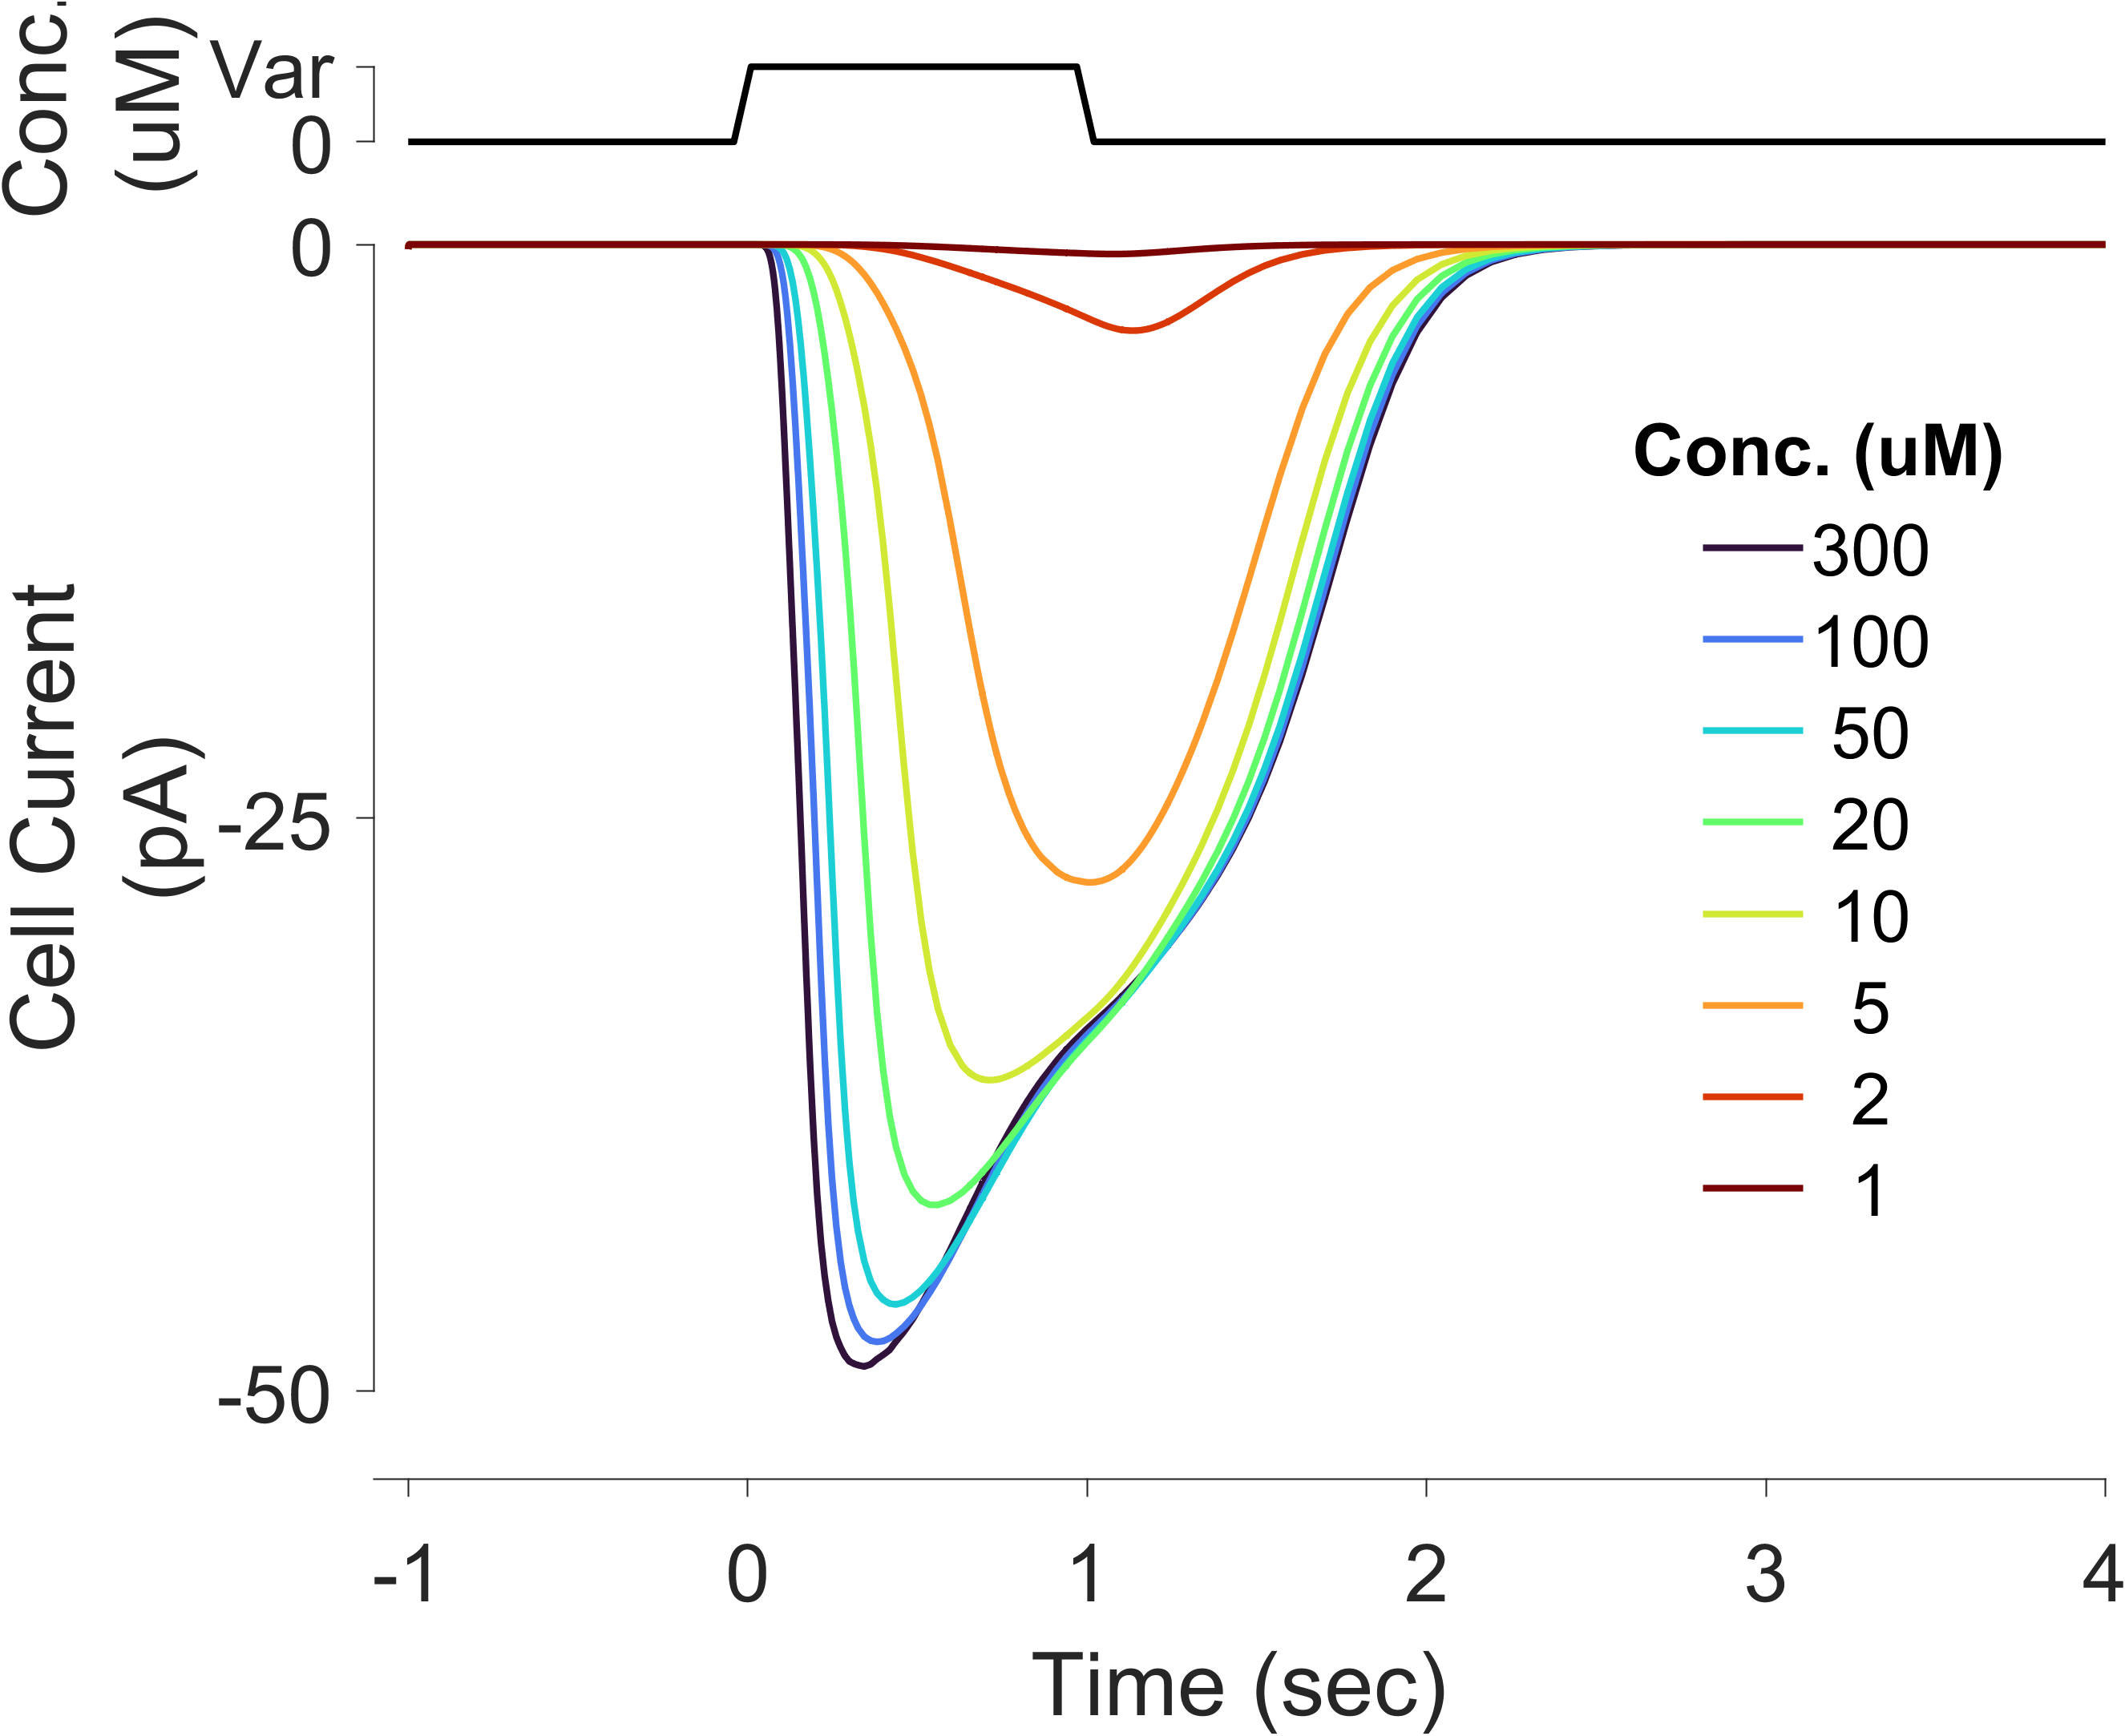
\includegraphics[width=0.5\linewidth]{figs/v1/fig_txn_compare_conc} }\subfloat[Quantification\label{fig:txCon-2}]{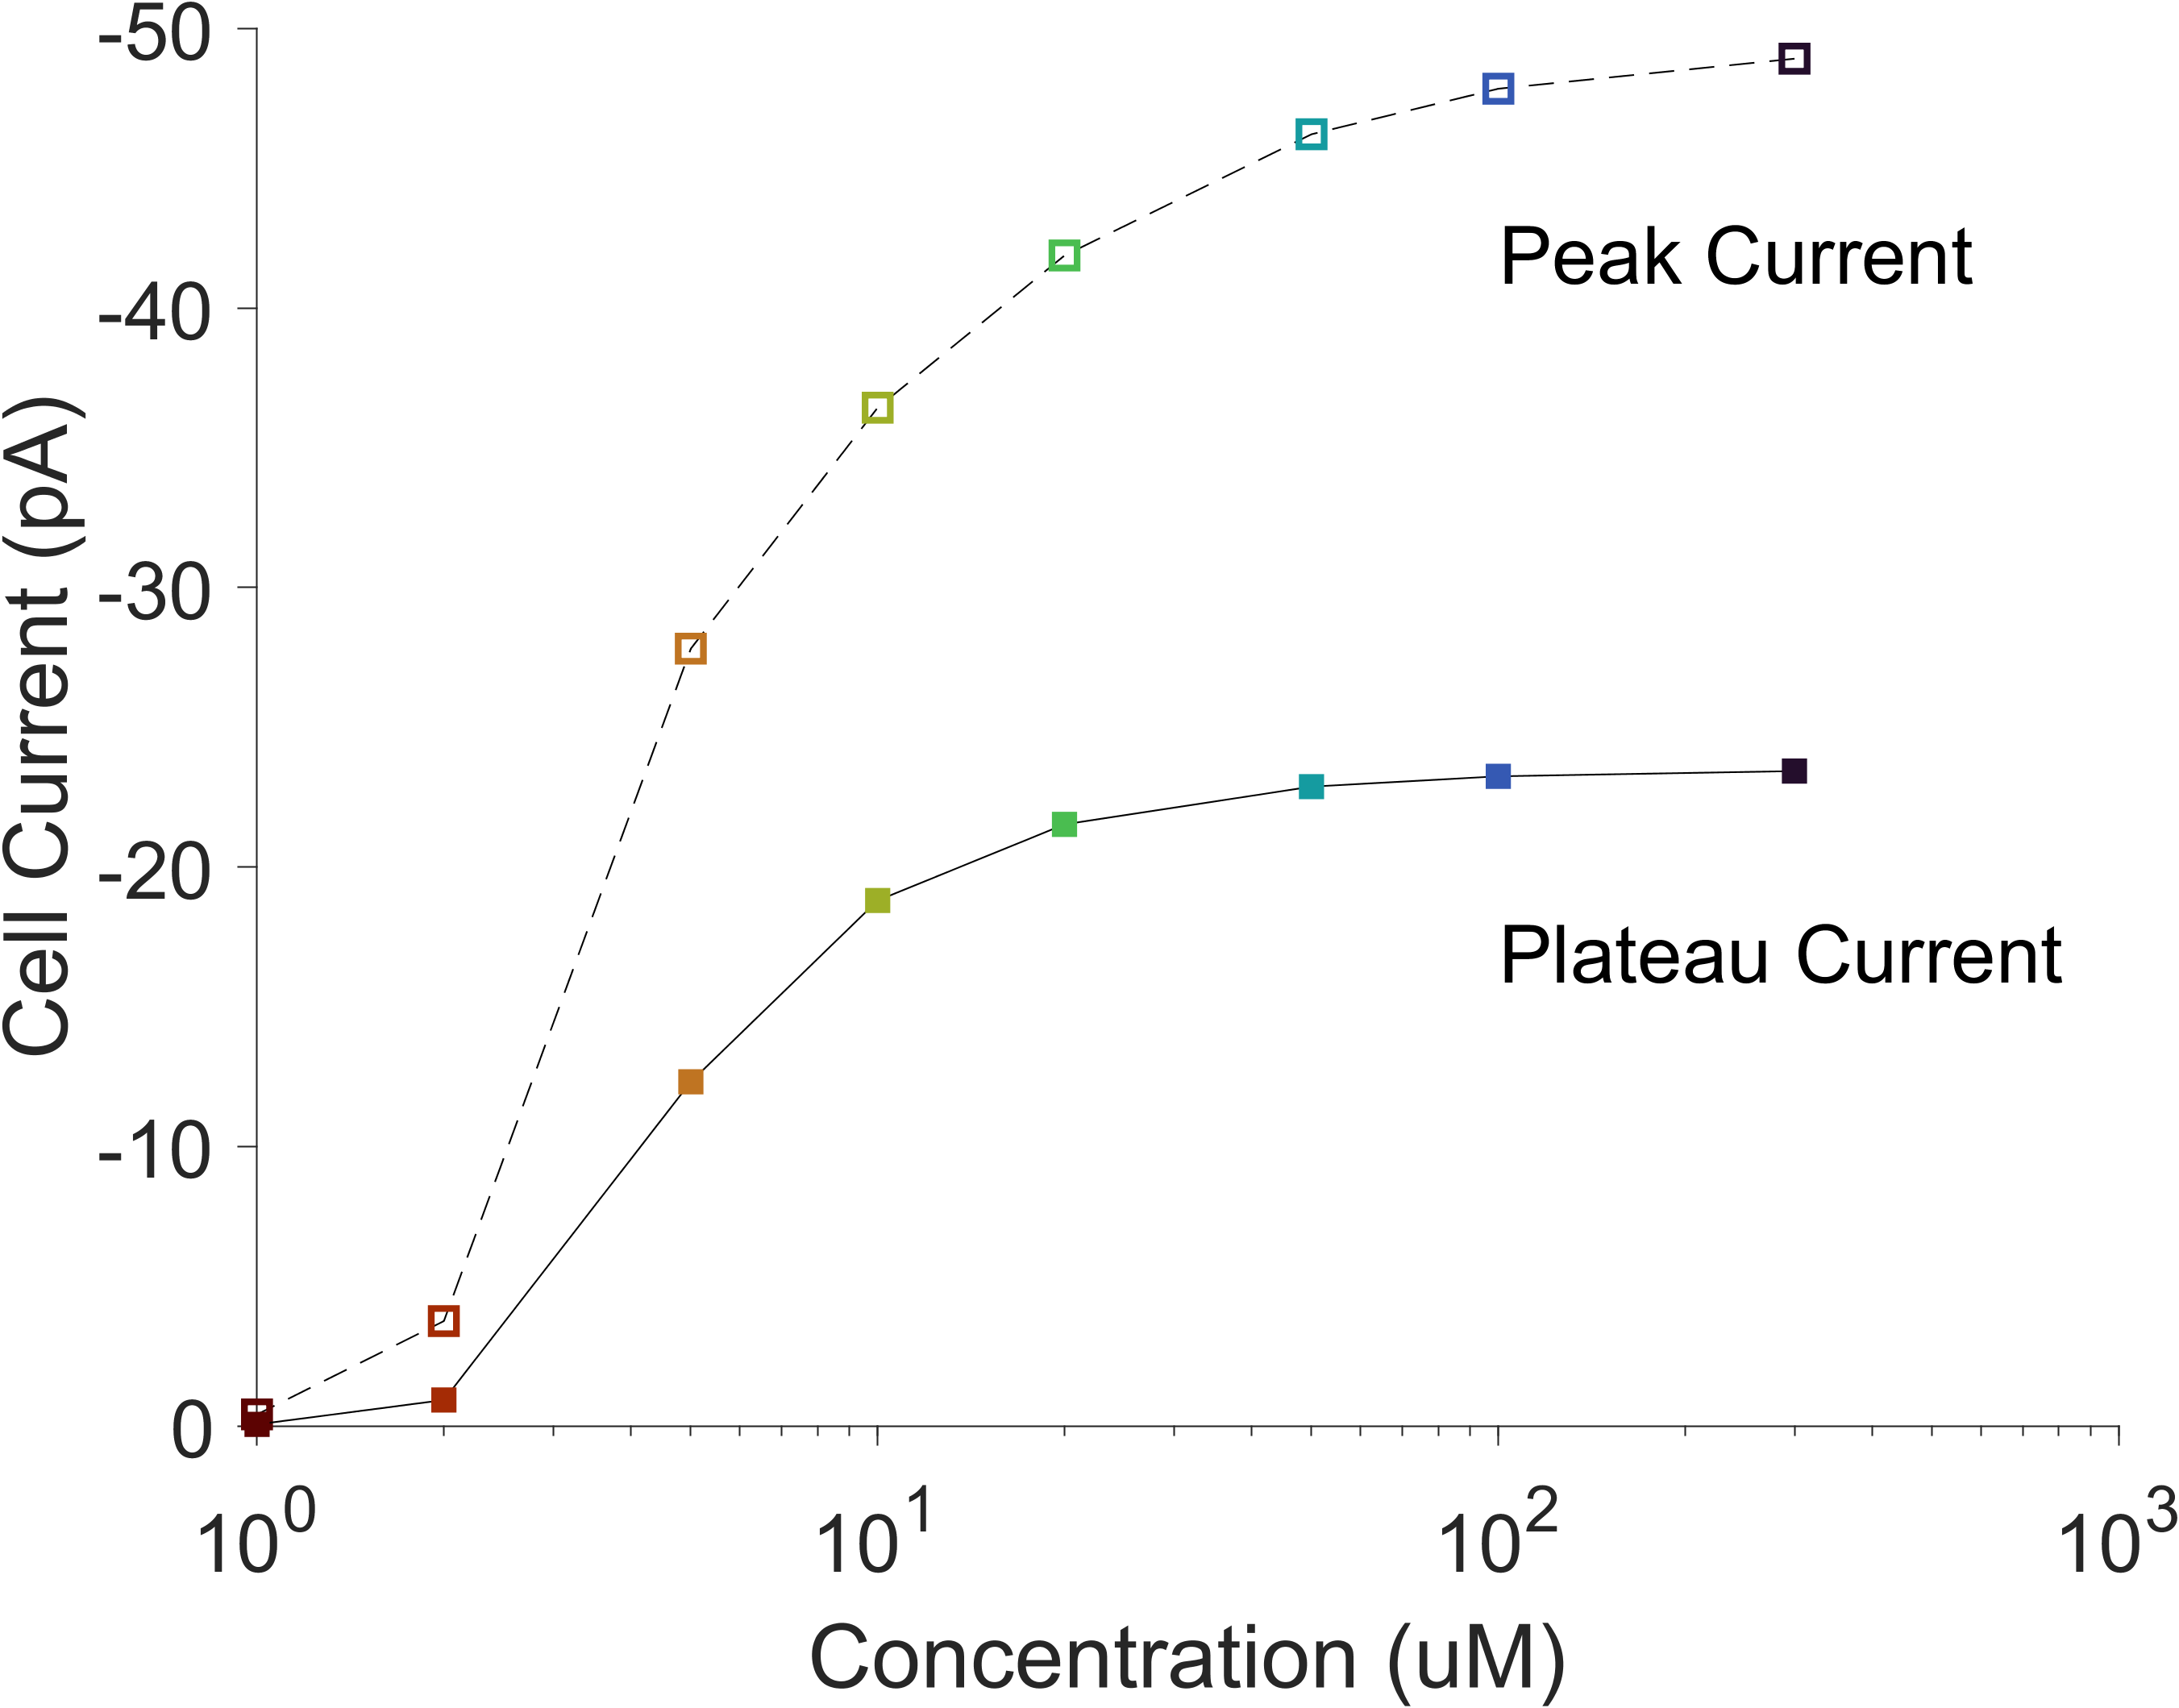
\includegraphics[width=0.5\linewidth]{figs/v1/fig_txn_compare_conc_quant} }

}

\caption{Transduction comparison for various odor concentration}\label{fig:txCon}
\end{figure}

Figure-\ref{fig:txCon}(a) shows odor-transduction response for 1 second long stimulus pulse at various concentrations. And, (b) compares the plateau current (measured at 1.5 sec) and peak current for a given stimulus. (Experimental data in Fig-\ref{fig:r99f24})

\hypertarget{ligand-receptor-binding-and-g-protein-activation-modeling}{%
\paragraph*{Ligand-receptor binding and G-protein activation modeling}\label{ligand-receptor-binding-and-g-protein-activation-modeling}}
\addcontentsline{toc}{paragraph}{Ligand-receptor binding and G-protein activation modeling}

In the equation for a single pulse of odor-stimulus (\(O_{\rm stim}\)), \(H(.)\) is the Heaviside step function and od represents odor-concentration. Parameters for the odorant-binding proportion \(\mathbf{bLR}\) equation are the following : k1=0.1143, r1=3.1663, and normalized maximum receptor count, Rtot = 1. Similarly, for \(\mathbf{aG}\), Gtot=1, k2=12.9344 and r2=6.5597.

\begin{equation}\label{eq:tx1}
\begin{split}
O_{\rm stim} &= {\rm od} \cdot [ H(t-t_0) - H(t-t_1) ];\ \ \ \ \  \text{(single pulse)}  \\
\frac{d\ \mathbf{bLR}}{dt} &= {\rm k1} \cdot O_{\rm stim} \cdot ({\rm Rtot} - \mathbf{bLR}) - {\rm r1} \cdot \mathbf{bLR} \\
\frac{d\ \mathbf{aG}}{dt} &= {\rm k2} \cdot \mathbf{bLR} \cdot ({\rm Gtot} - \mathbf{aG}) - {\rm r2} \cdot \mathbf{aG}
\end{split}
\end{equation}

\hypertarget{intracellular-signalling-and-adaptation}{%
\paragraph*{Intracellular signalling and adaptation}\label{intracellular-signalling-and-adaptation}}
\addcontentsline{toc}{paragraph}{Intracellular signalling and adaptation}

\begin{figure}

{\centering 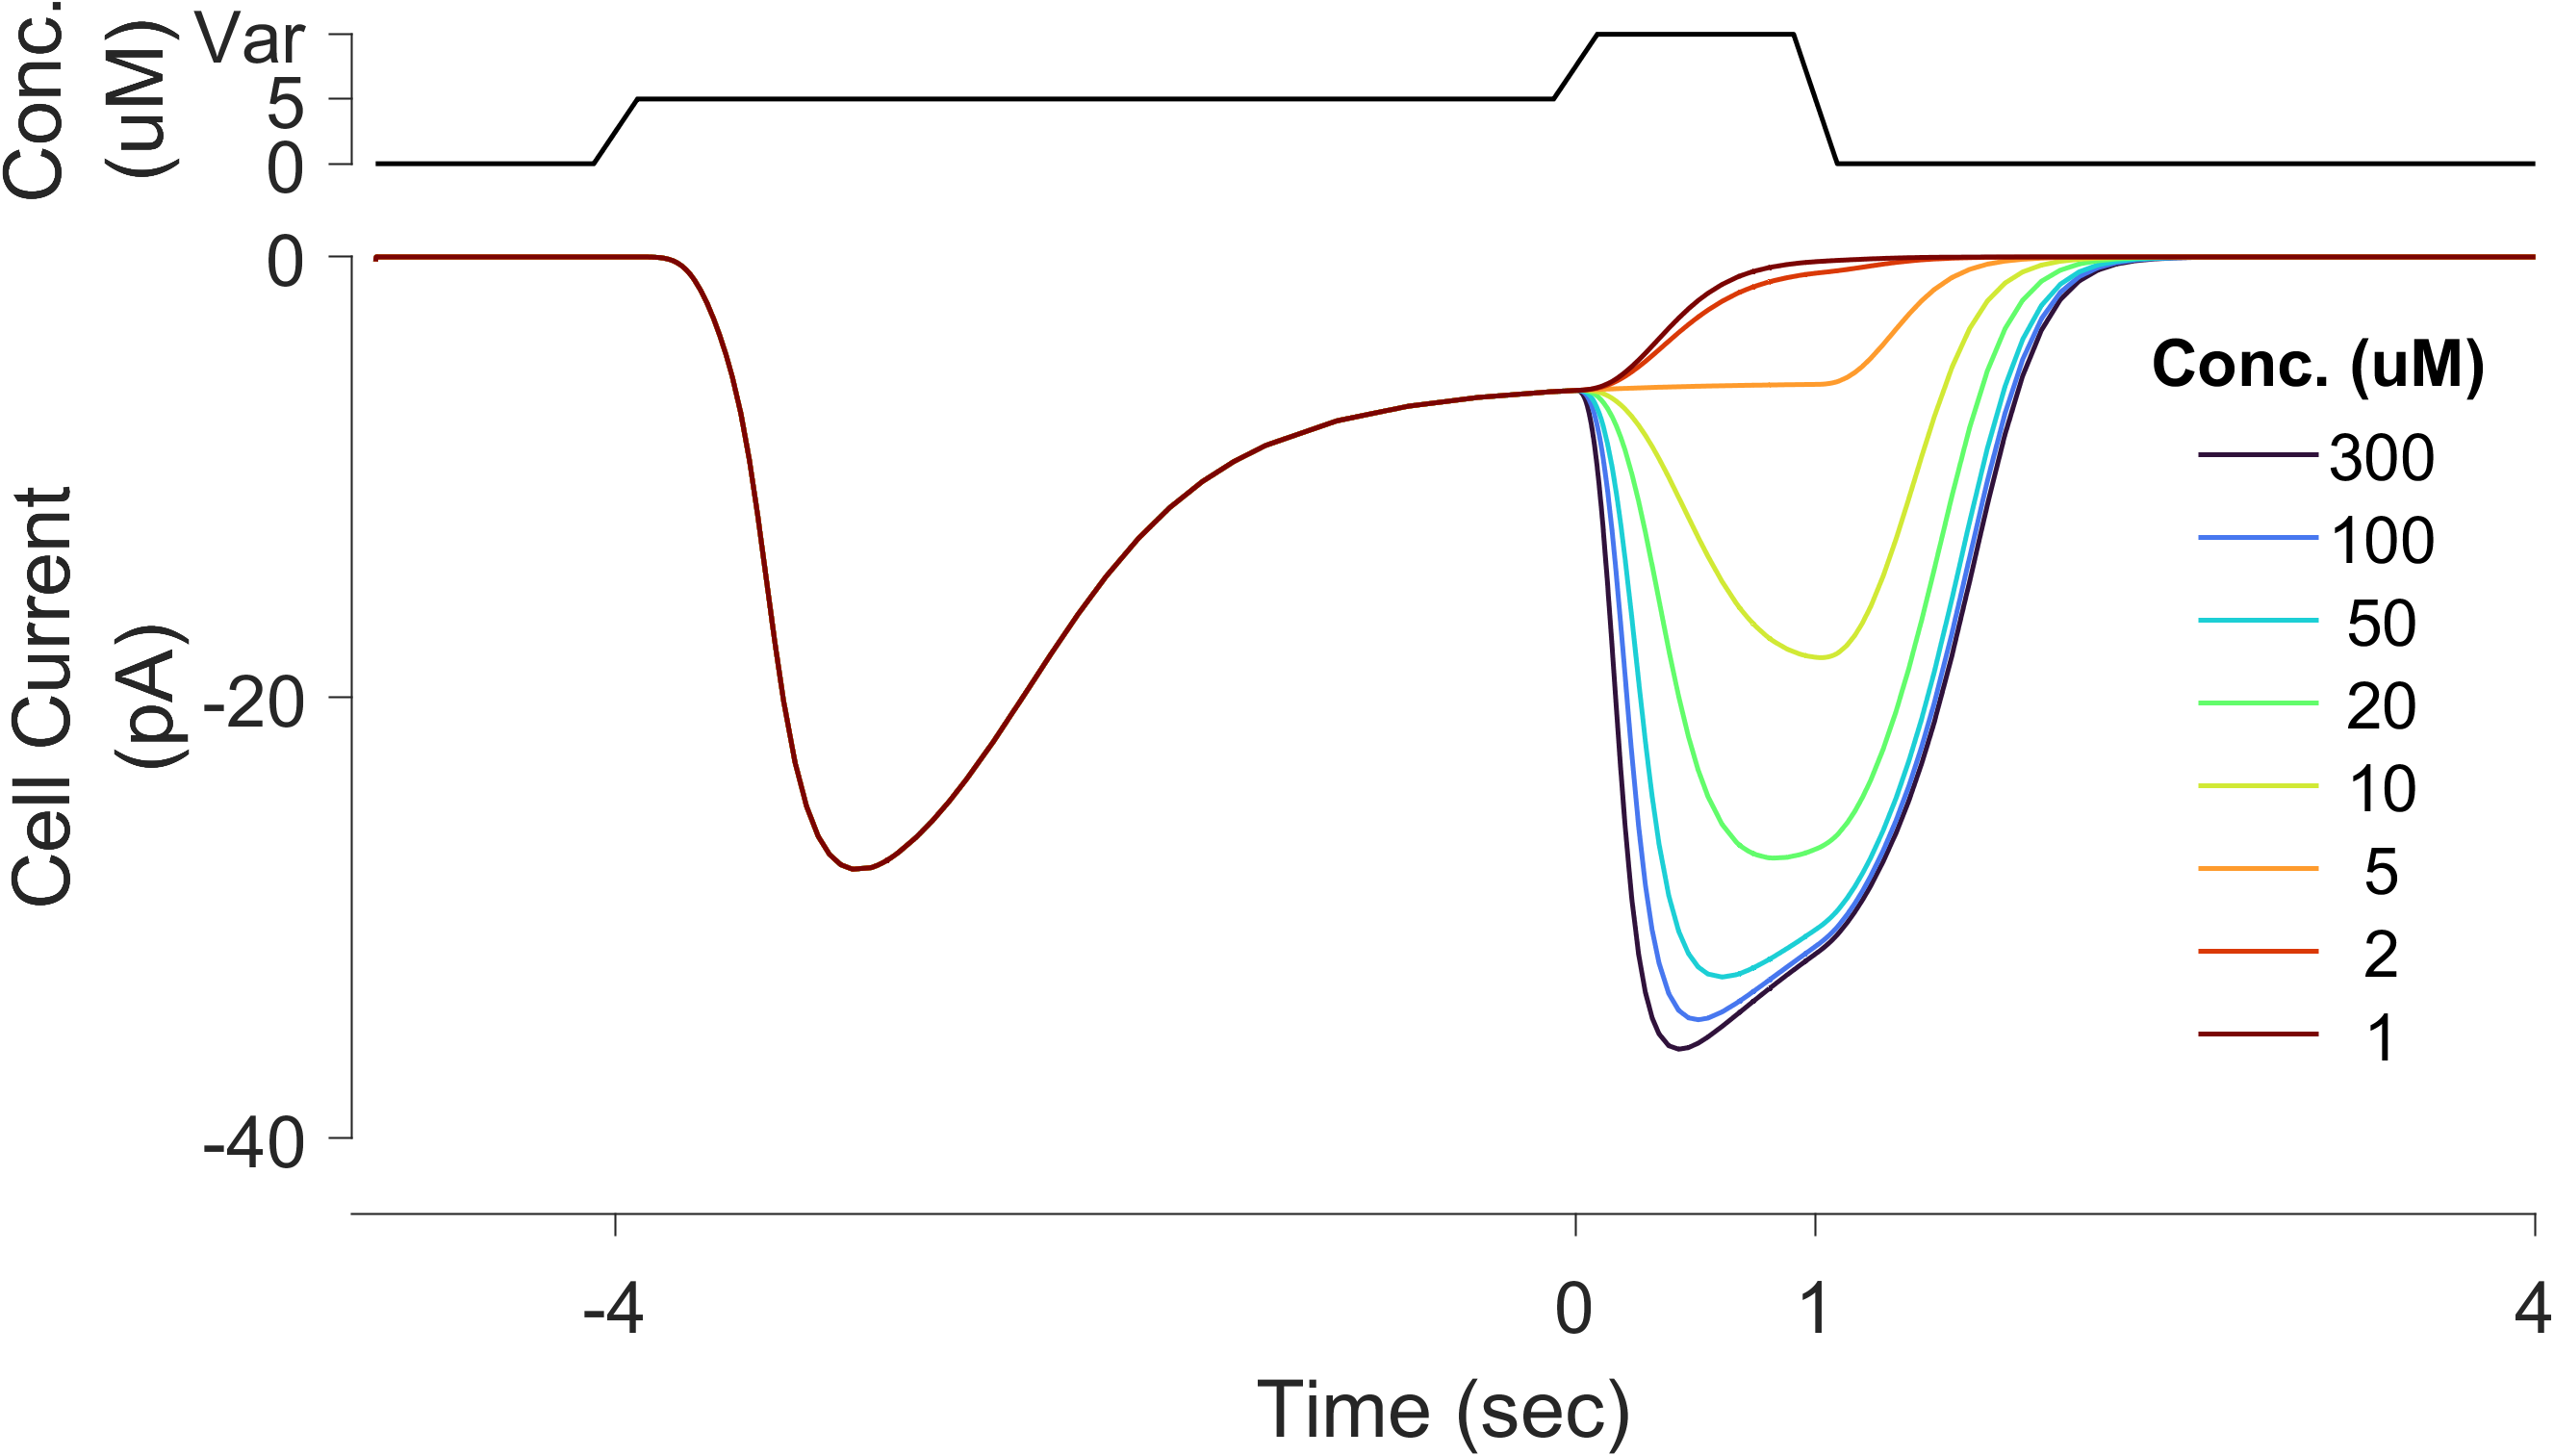
\includegraphics[width=0.7\linewidth]{figs/v1/fig_txn_compare_adaptation} 

}

\caption{Adaptation in transduction comparison for the test-pulse of different concentrations}\label{fig:txAdp}
\end{figure}

Figure-\ref{fig:txAdp} demonstrates olfactory adaptation due to a 4 seconds long low concentration (5uM) pre-stimulus pulse. Response of the following test-pulse of 1 second shows that it requires about 4 times stronger (20uM) stimulus to get similar current output, demonstrating sensory adaptation. (Experimental data in Fig-\ref{fig:r99f24})

\begin{equation}\label{eq:tx2}
\begin{split}
\frac{d\ \mathbf{cAMP}}{dt} &= synth - {\rm pd} \cdot \mathbf{cAMP} \\
\frac{d\ \mathbf{Ca}}{dt} &= {\rm inf}\cdot I_{\rm CNG} - J_{\rm NCX} - ({\rm cc1} \cdot \mathbf{Ca} - {\rm cc2} \cdot \mathbf{CaCaM}) \\
\frac{d\ \mathbf{CaCaM}}{dt} &= {\rm cc1} \cdot \mathbf{Ca} - {\rm cc2} \cdot \mathbf{CaCaM} \\
\frac{d\ \mathbf{aCaMK}}{dt} &= {\rm ck1} \cdot \mathbf{CaCaM} - {\rm ck2} \cdot \mathbf{aCaMK} \\
\frac{d\ \mathbf{IX}}{dt} &= {\rm cx1} \cdot \mathbf{Ca} - {\rm cx2} \cdot \mathbf{IX} \\
& synth = \frac{\mathbf{aG} \cdot {\rm smax}}{1 + (\mathbf{aCaMK} / {\rm kinh} )^{\rm ninh}} \\
& J_{\rm NCX} = {\rm ef}\cdot \mathbf{Ca}/[1+(\mathbf{IX}/{\rm kI})^{\rm nI}] \\
\end{split}
\end{equation}

Equations-\eqref{eq:tx2} are responsible for intracellular calcium mediated signaling that is responsible for transduction adaptation. \(I_{\rm CNG}\) represents depolarizing \(Ca^{2+}\)-ion current through cyclic nucleotide-gated (CNG) channels, and \(J_\mathbf{NCX}\) is the \(Ca^{2+}\)-ions flux through Na/Ca exchanger (NCX). Whereas, \(\mathbf{IX}\) is a mathematical \(Ca^{2+}\)-ion stimulated intermediate substance.

Here are the parameters used : pd=7.5749, smax=45.5118, kinh=1.0018, ninh=1.3081 (for \(\mathbf{cAMP}\)); inf=1.7619, cc1=0.7750, cc2=26.3950 (for \(\mathbf{Ca}\) and \(\mathbf{CaCaM}\)); cnmax=0.9663, vcng=0.0106, hmc1=1.4829, n1=3.1844, inhmax=3.5697, kinhcng=0.5181, ninhcng=1.4511 (for \(I_\mathbf{CNG}\)), ef=2.7583, kI=10.0453, nI=1.9848 (for \(J_\mathbf{NCX}\)); ck1=8.5342, ck2=0.3069 (for \(\mathbf{aCaMK}\)); cx1=1.2307, cx2=10.9297 (for \(\mathbf{IX}\)).

\hypertarget{effector-channel-activity-and-cell-currents-for-transduction}{%
\paragraph*{Effector Channel Activity and cell currents for transduction}\label{effector-channel-activity-and-cell-currents-for-transduction}}
\addcontentsline{toc}{paragraph}{Effector Channel Activity and cell currents for transduction}

\begin{equation}
\begin{split}
\frac{d\ \mathbf{V_{ORN}}}{dt} &= \frac{1}{\rm cap} \cdot (\ I_{\rm CNG} + I_{\rm Cl(Ca)} + I_{\rm leak}\ ) + {\rm revCp} \cdot \mathbf{\dot{V}_{ML}} \\
I_{\rm CNG} &= \frac{{\rm cnmax} \cdot \mathbf{cAMP}^{\rm n_1} \cdot ({\rm vcng}-\mathbf{V_{ORN}})}{\mathbf{cAMP}^{\rm n_1} + (inhcng \cdot {\rm hmc_1})^{\rm n_1}} \\
& inhcng = 1 + \frac{({\rm inhmax}-1)\cdot \mathbf{CaCaM}^{\rm ninhcng}}{\mathbf{CaCaM}^{\rm ninhcng} + {\rm kinhcng}^{\rm ninhcng}} \\
I_{\rm Cl(Ca)} &= \frac{{\rm clmax} \cdot \mathbf{Ca}^{\rm n_2} \cdot ({\rm vcl} - \mathbf{V_{ORN}})}{\mathbf{Ca}^{\rm n_2} + {\rm hmc_2^{n_2}}} \\
I_{\rm leak} &= {\rm gl} \cdot ({\rm vl} - \mathbf{V_{ORN}})
\end{split}
\end{equation}

\(\mathbf{V_{ORN}}\) is a sum of the resultant transduction voltages (with cap=0.0039). ML Spike-voltage (see \(\S\)\ref{ML}) is connected through (revCp=0.3). The resulting total leak current is \(I_{\rm leak}\) (with gl=4.9195, vl=-44.0413). \(I_{\rm Cl(Ca)}\) is an outward chlorine current through \(Ca^{2+}\) activated chloride channels (Ca(Cl)) (with parameters : clmax=0.9397, vcl=-7.7902 hmc2=2.7678, n2=3.1128).

\hypertarget{ML}{%
\subsection{ML spikes}\label{ML}}

Modified Morris-Lecar (ML) model is used to generate fast voltage dynamics to represent action potential in ORN to match experimental data (Reisert and Matthews 1999).

\begin{figure}

{\centering 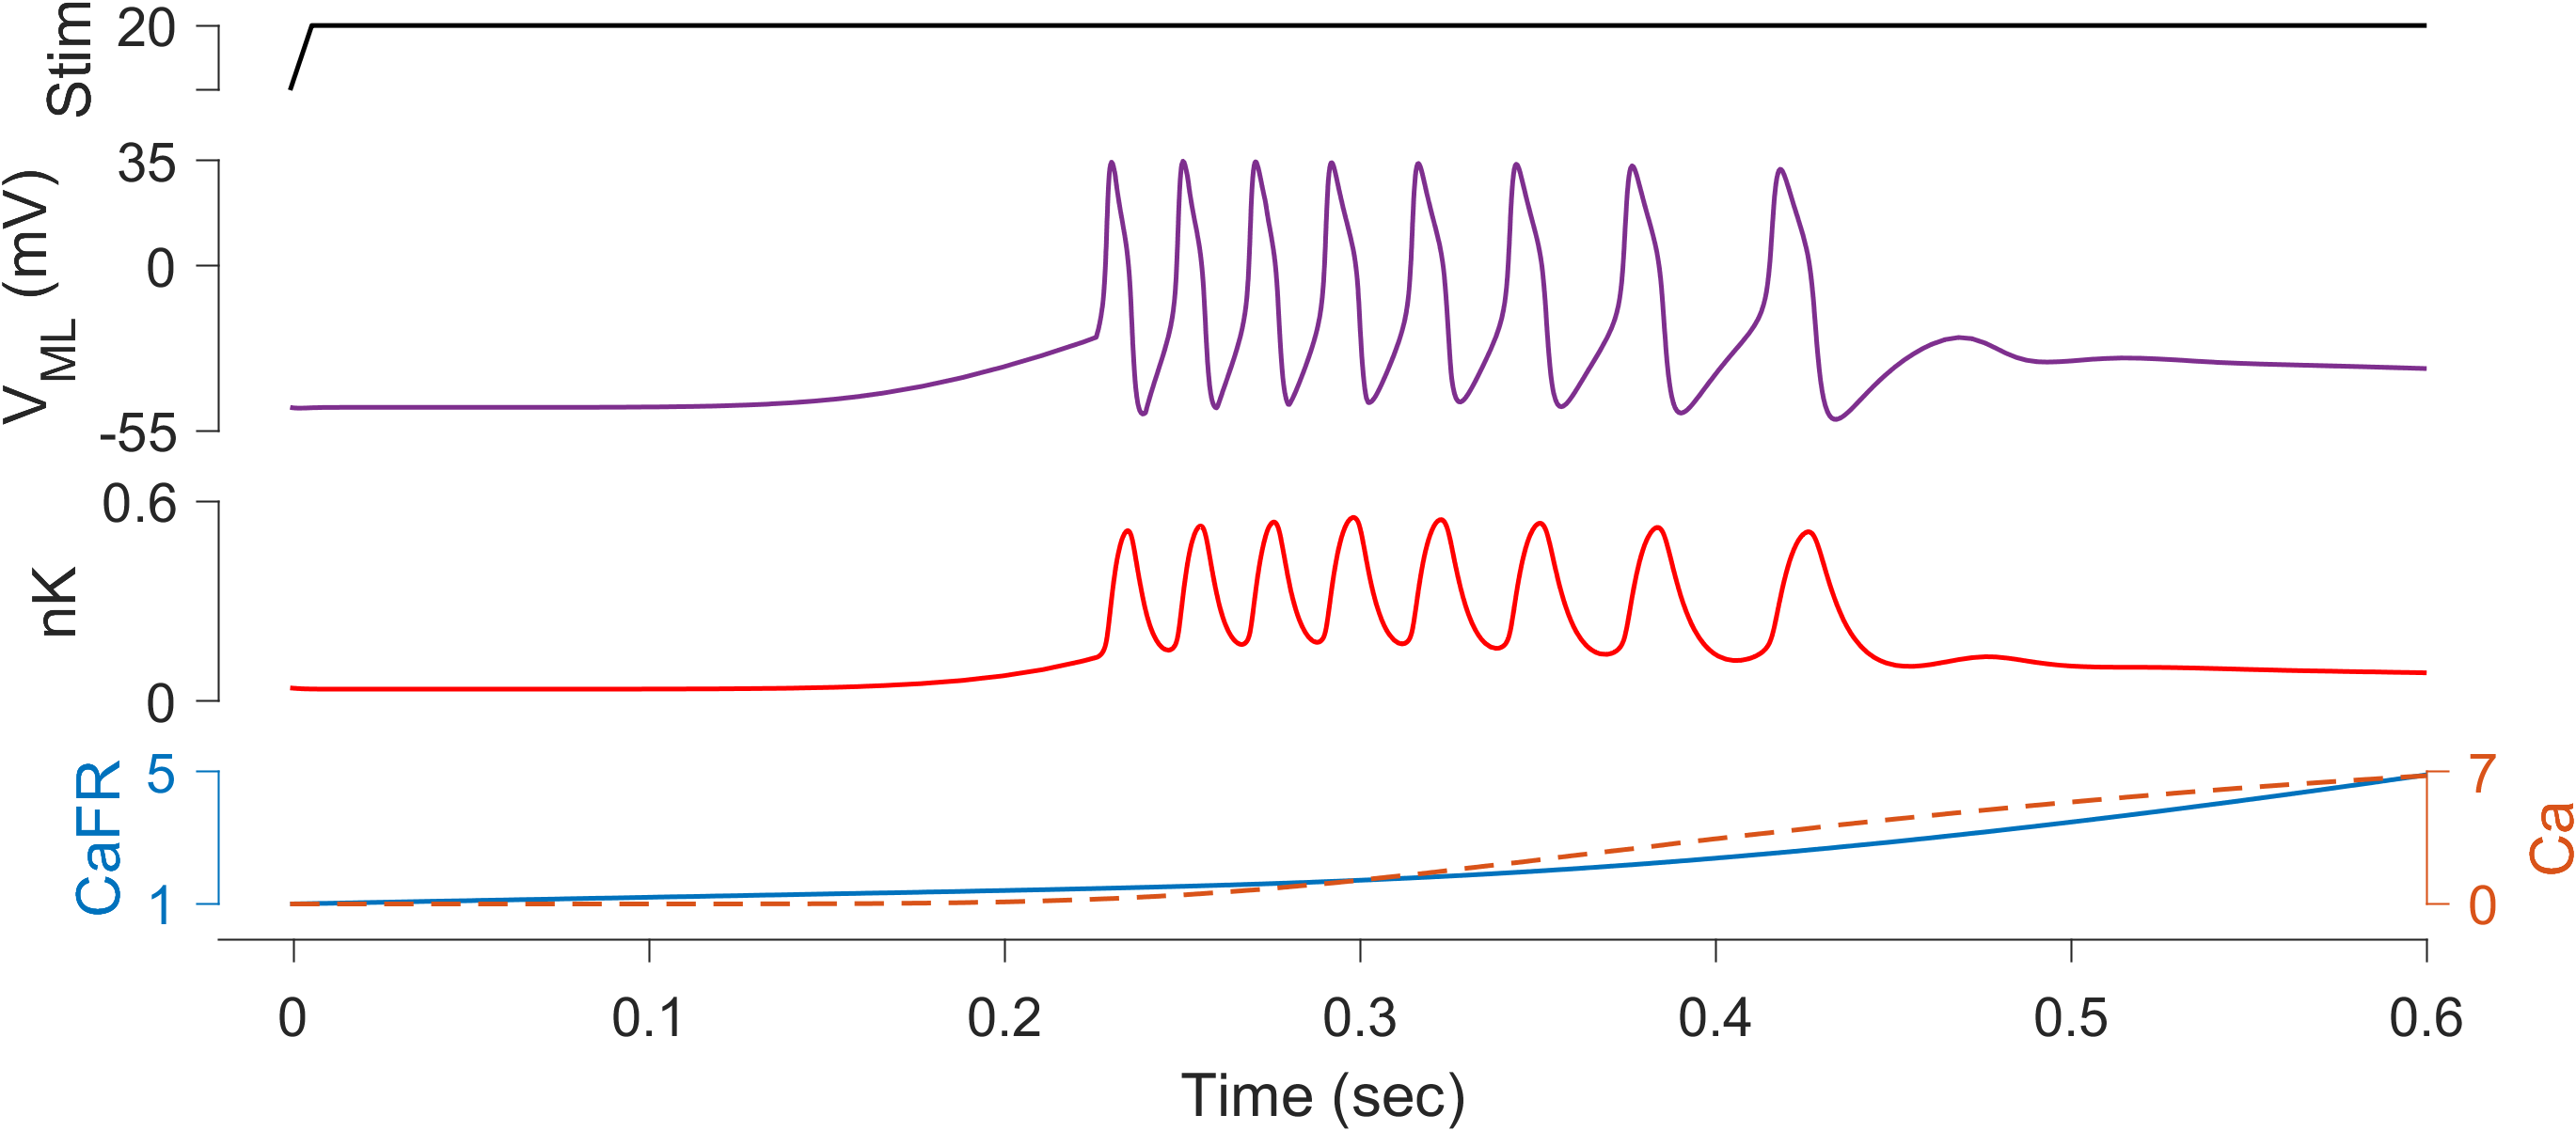
\includegraphics[width=0.9\linewidth]{figs/v1/fig_ML_spikes} 

}

\caption{Altered Morris-Lecar model for action potentials in ORN}\label{fig:MLspk}
\end{figure}

Figure-\ref{fig:MLspk} shows all three components used to model ML spikes in ORN (Equation- \eqref{eq:MLeq}). Model equations and parameters used in \(\mathbf{V_{ML}}\) and \(\mathbf{nK}\) are from Anderson, Ermentrout, and Thomas (2015). vL is changed from -60mV to -44mV to match the resting potential of ORN model. (ML parameters:Eq-\eqref{eq:MLpar}, ML functions:Eq-\eqref{eq:MLfxn}).

\(\mathbf{CaFR}\) is introduced to model adaption-encoding in firing rate for spiking ORN and added to the ML model via \(ct\) (with maxFR=50, indicating 50Hz as a maximum firing rate of ORN). Other parameters are p=2, n=100, and m=1. I am also adding two values dependent on the transduction model : intracellular \(Ca^{2+}\)-driven current, \(I_{\rm Ca}\) (with gain gIca=10), and other ionic currents during a spiking event, \(I_{\rm ions}\) (with spkThr=-43mV and gain gIion=22).

\begin{equation} \label{eq:MLeq}
\begin{split}
\frac{d\ \mathbf{V_{ML}}}{dt} &= \frac{ct}{\rm C_m} \cdot [ I_{\rm ions} + I_{\rm Ca} - {\rm gL} \cdot (\mathbf{V_{ML}} - {\rm v_L}) - {\rm gK} \cdot \mathbf{nK} \cdot (\mathbf{V_{ML}}-{\rm v_K}) \\
&\ \  - {\rm gCa} \cdot m_\infty(\mathbf{V_{ML}}) \cdot (\mathbf{V_{ML}}- {\rm v_{Ca}}) \ ] \\
\frac{d\ \mathbf{nK}}{dt} &= \frac{ct \cdot [ n_\infty(\mathbf{V_{ML}}) - \mathbf{nK} ]}{\tau(\mathbf{V_{ML}})} \\
\frac{d\ \mathbf{CaFR}}{dt} &= (1+\mathbf{Ca})*({\rm p}(\mathbf{\dot{Ca}} > 0) - {\rm n}(\mathbf{\dot{Ca}}<0\  \& \ \mathbf{CaFR} > {\rm m})) \\
 \mathbf{I_{ORN}} &= {\rm gl} \cdot ({\rm vl} - \mathbf{V_{ORN}})
\end{split}
\end{equation}

\begin{equation} \label{eq:MLpar}
\begin{split}
& ct = \frac{100\cdot {\rm maxFR}}{\mathbf{CaFR}},\ I_{\rm Ca} = {\rm \frac{gI_{Ca} \cdot \dot{Ca}}{1 + Ca}},\ I_{\rm ions}={\rm gIons (\mathbf{V_{ORN}} > spkThr )} \\
& {\rm v_{Ca}=120\ mV,\ v_K=-84\ mV,\ v_L=-60\ mV,\ C_m=20\ \mu F/cm^2,} \\ 
& {\rm g_{Ca}=4.4\ m\mho/cm^2,\ g_K=8\ m\mho/cm^2,\ g_L=2\ m\mho/cm^2,}
\end{split}
\end{equation}

\begin{equation} \label{eq:MLfxn}
\begin{split}
\xi(v)=\frac{v-v_c}{v_d},\ &\alpha(v)=\frac{\phi \cosh(\xi/2)}{1+ e^{2\xi}},\ \beta(v)=\frac{\phi \cosh(\xi/2)}{1+ e^{-2\xi}}, \\
n_\infty(v) &= \frac{\alpha(v)}{\alpha(v)+\beta(v)}\ =\  \frac12(1 + \tanh \xi) \\
\tau(v) &= \frac{1}{\alpha(v) + \beta(v)}\ =\  \frac{1}{\phi \cosh(\xi/2)} \\
m_\infty&(v) = \frac12\left(1+ \tanh(\frac{v-v_a}{vb})\right) \\ 
\phi=0.04\ s^{-1};\ &v_a=-1.2,\ v_b=18,\ v_c=2,\ v_d=30\ {\rm mV}.
\end{split}
\end{equation}

\hypertarget{identifying-ml-spikes-added-in-orn}{%
\subsubsection{Identifying ML spikes added in ORN}\label{identifying-ml-spikes-added-in-orn}}

\begin{figure}

{\centering 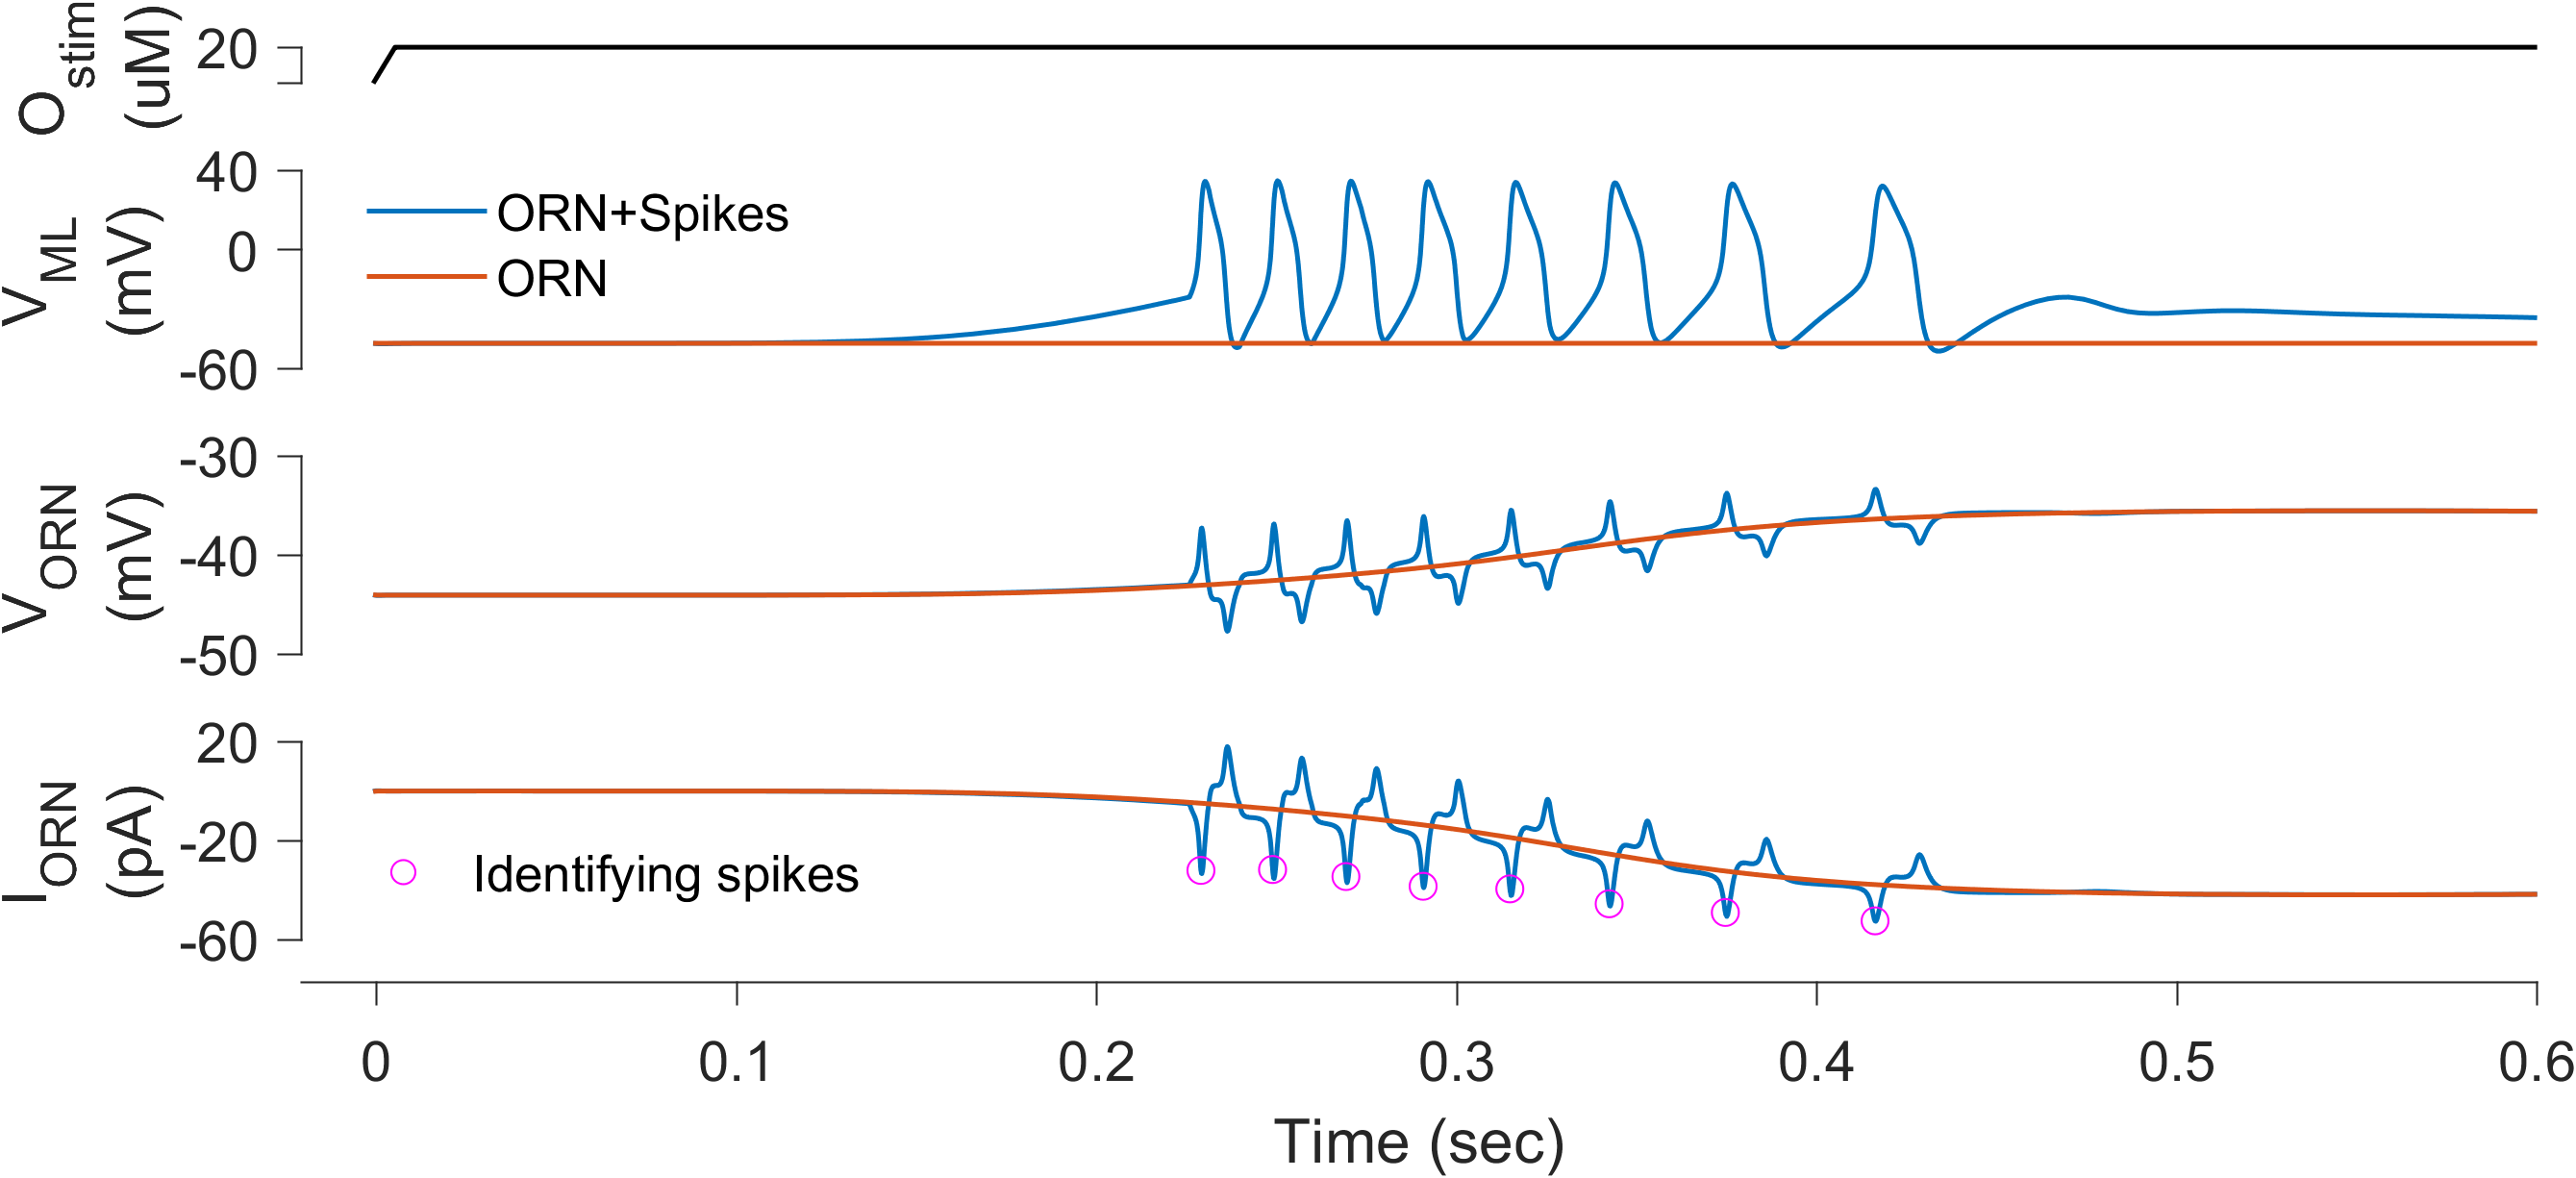
\includegraphics[width=0.9\linewidth]{figs/v1/fig_ML_spikes_with_ORN} 

}

\caption{Resuling ORN current due to Morris-Lecar spikes}\label{fig:MLspkORN}
\end{figure}

Figure-\ref{fig:MLspkORN} compares transduction voltages of a non-spiking ORN transduction (orange) with a spiking ORN (blue). The first panel is ML-voltage (\(V_{\rm ML}\)), which is added back to ORN transduction simulation (into \(V_{\rm ORN}\)) and eventually the predicted current (\(I_{\rm ORN}\)) will display the effects of ML spikes. Local-minima identification algorithm is used to identify spikes in ORN for the further study (as marked in last panel). Figure-\ref{fig:MLspkID} shows example of spike-identification for a low (20uM) and high (300uM) stimulus.

\begin{figure}

{\centering 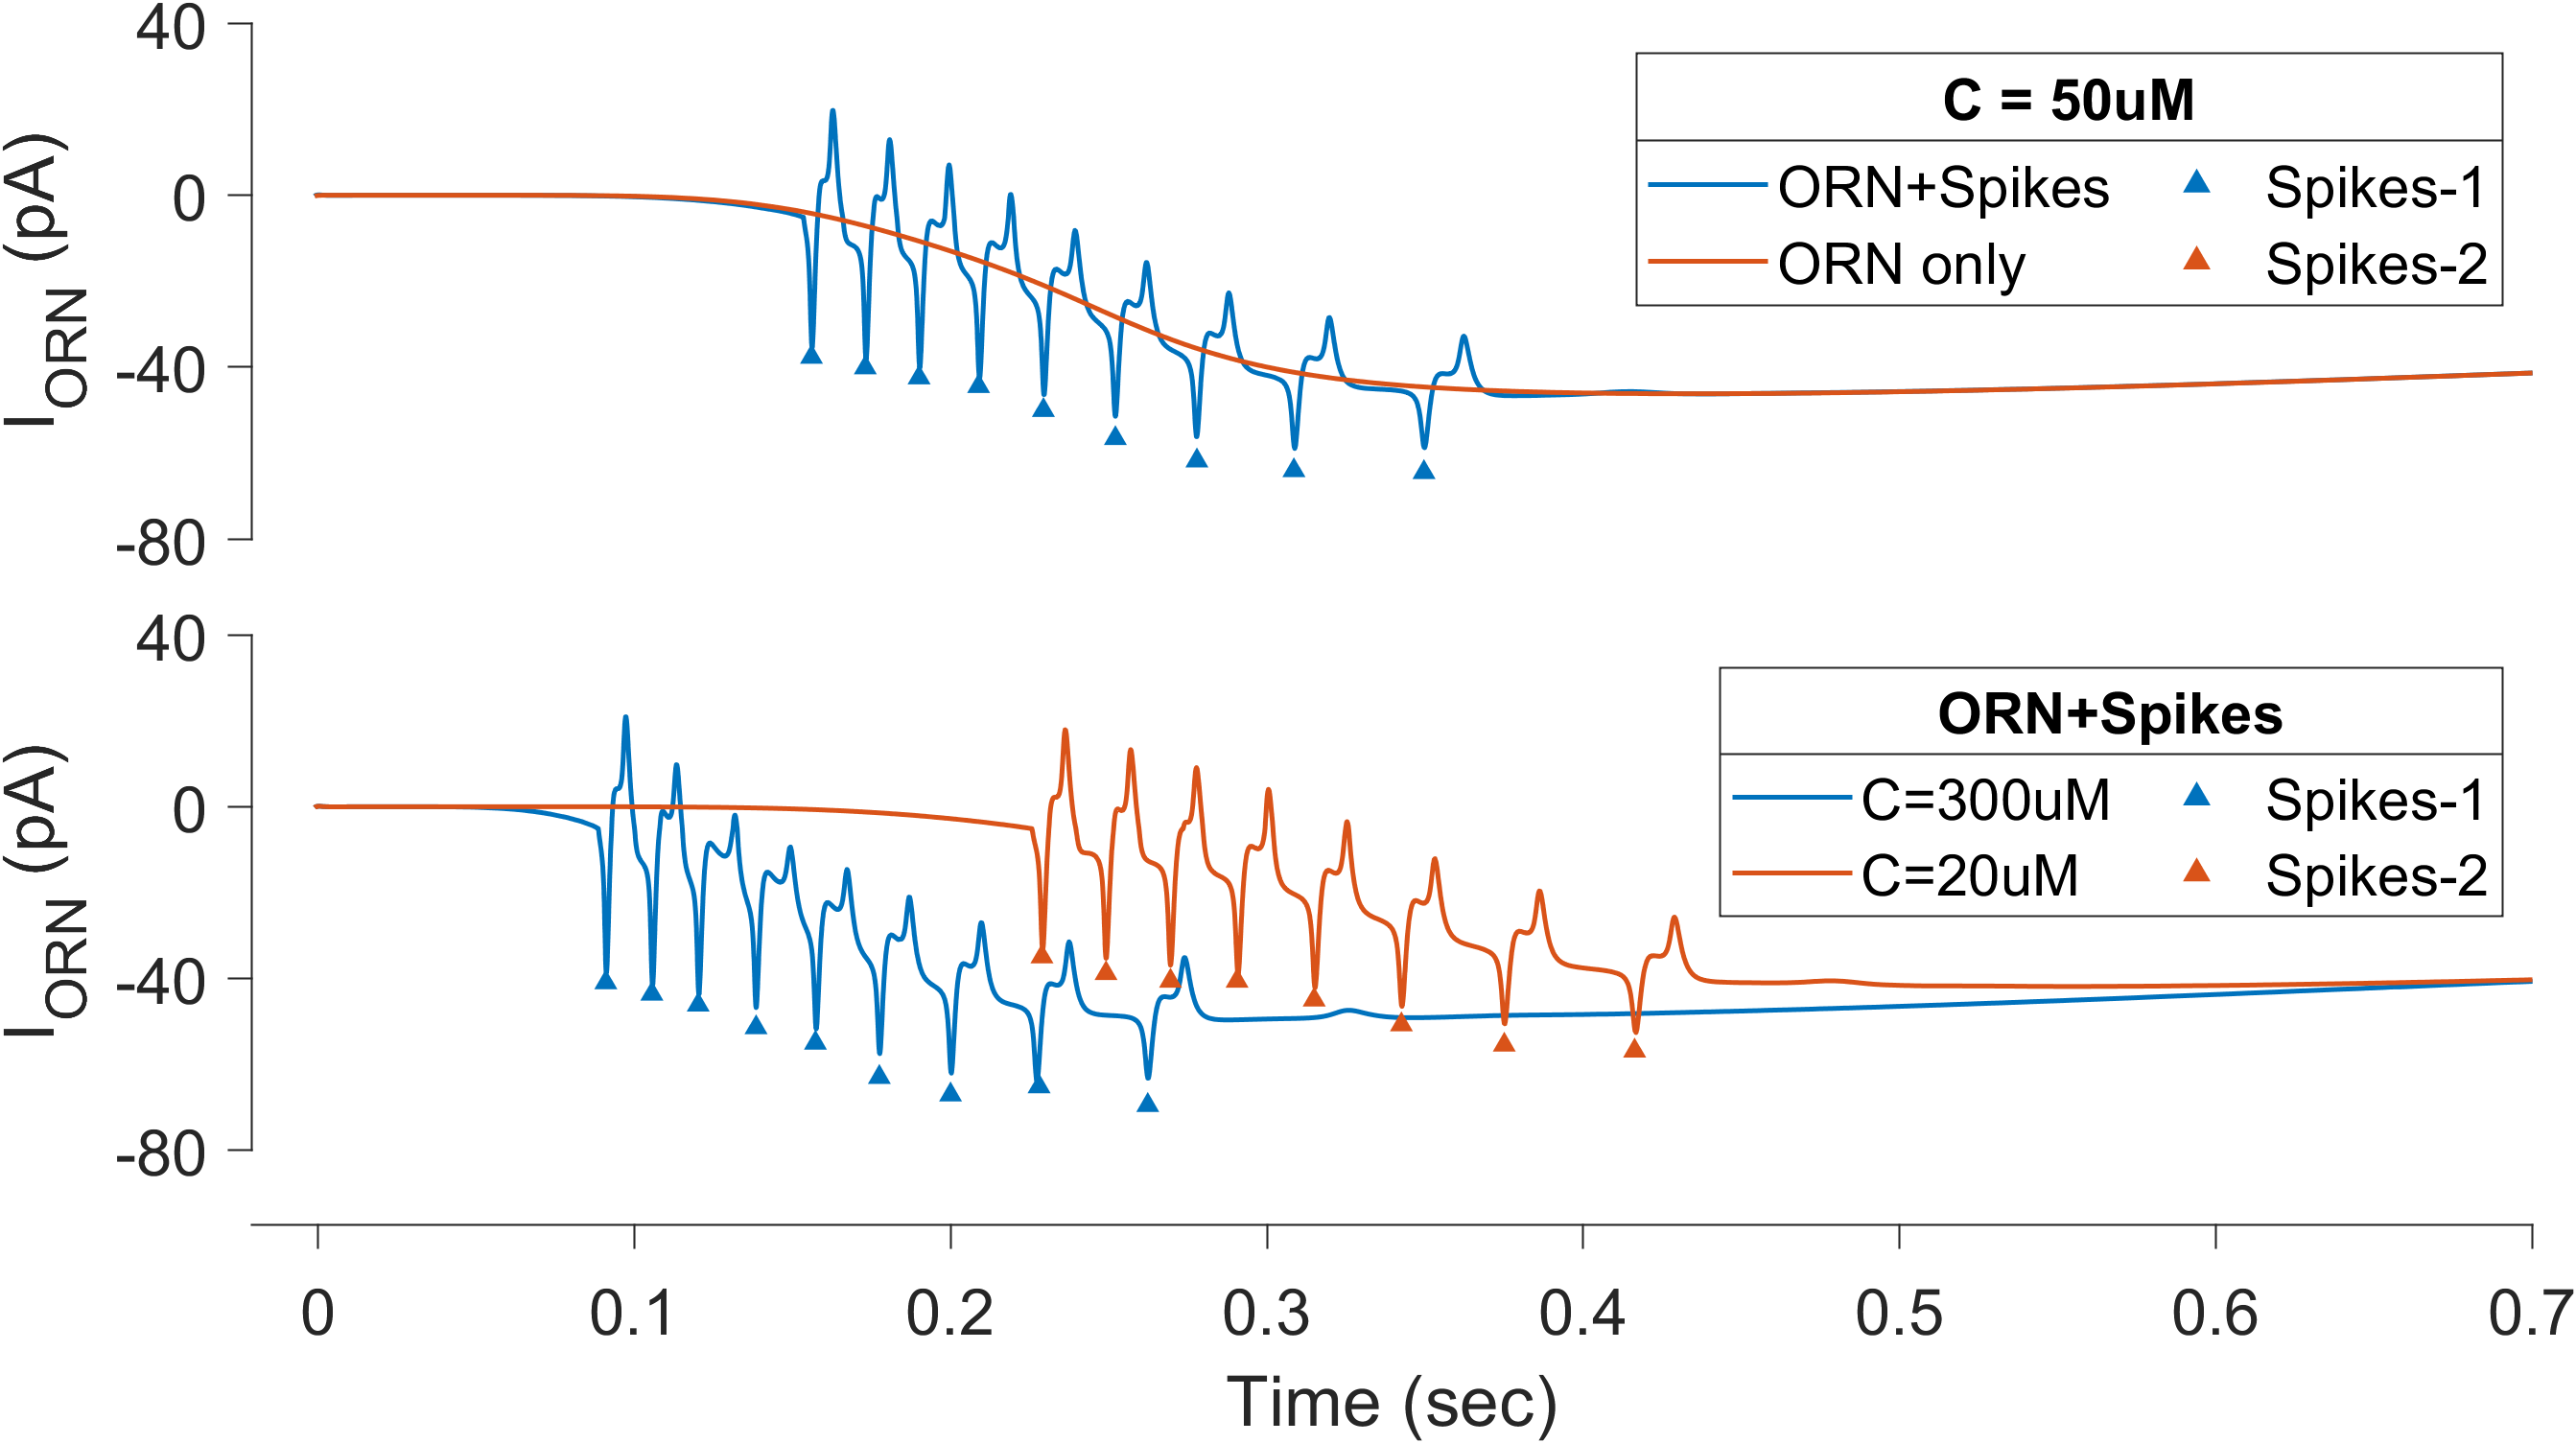
\includegraphics[width=0.8\linewidth]{figs/v1/fig_ML_spikes_ID} 

}

\caption{Robust identification of ML-spikes across stimulus concentration range}\label{fig:MLspkID}
\end{figure}

\hypertarget{sniffing-experiment}{%
\subsection{Sniffing experiment}\label{sniffing-experiment}}

\begin{figure}

{\centering 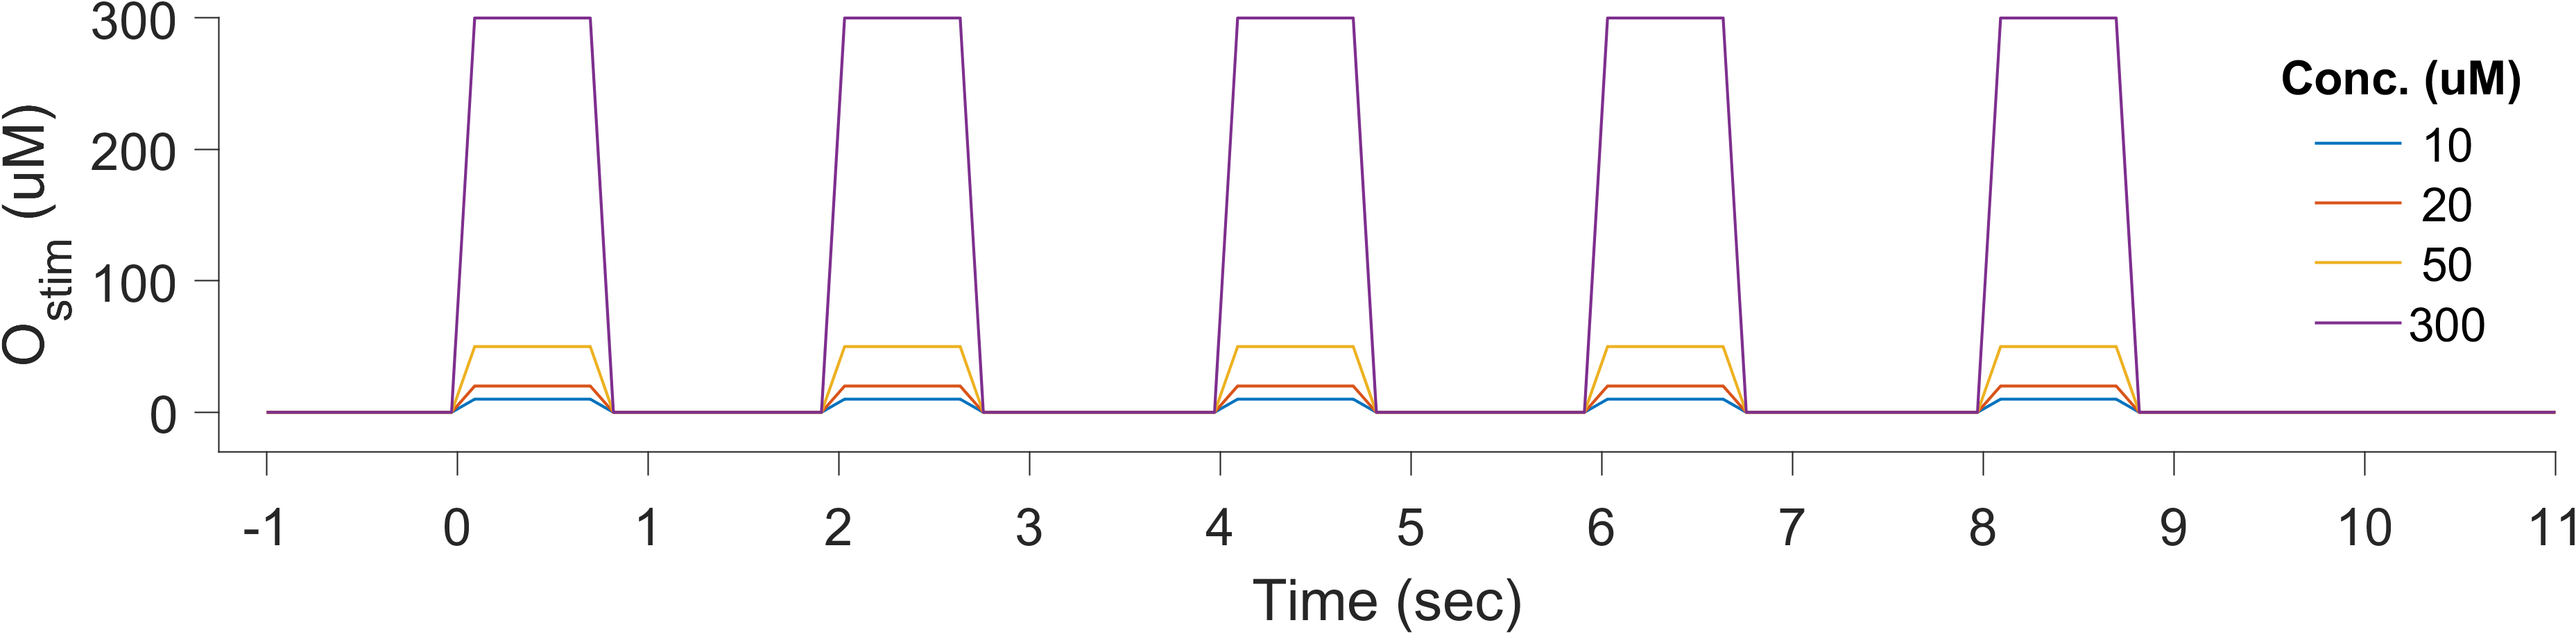
\includegraphics[width=0.9\linewidth]{figs/v1/fig_sniff_pulse} 

}

\caption{Example stimulus of 30 breaths/min used in sniffing experiment}\label{fig:pulse}
\end{figure}

To simulate breathing, I am using continuous pulses of 33\% duty cycle (Zak et al. 2018) of 4 different concentrations (10,20,50 and 300 uM). First-pulse's response is the peak-response and fifth-pulse's response is taken as the steady-state response as the response does not change after the first two pulses (see Appendix C). Figure-\ref{fig:pulse} displays the odor-stimulus for 30bpm used in frog spiking-ORN sniffing experiments.

\hypertarget{results}{%
\section{Results}\label{results}}

\hypertarget{spiking-in-orn}{%
\subsection{Spiking in ORN}\label{spiking-in-orn}}

Spiking in the ORN model was achieved. Figure-\ref{fig:rORN} shows a simulation of three stimulus of two pulses each with varying concentrations (blue-30,5; red-5,30; yellow-0,0). Effect of adaption is higher in blue, which has stronger stimulus (30uM) first and followed by 5uM pulse. Identified spikes are labeled with an upwards pointing triangle in \(I_{\rm ORN}\) panel.

\begin{figure}

{\centering 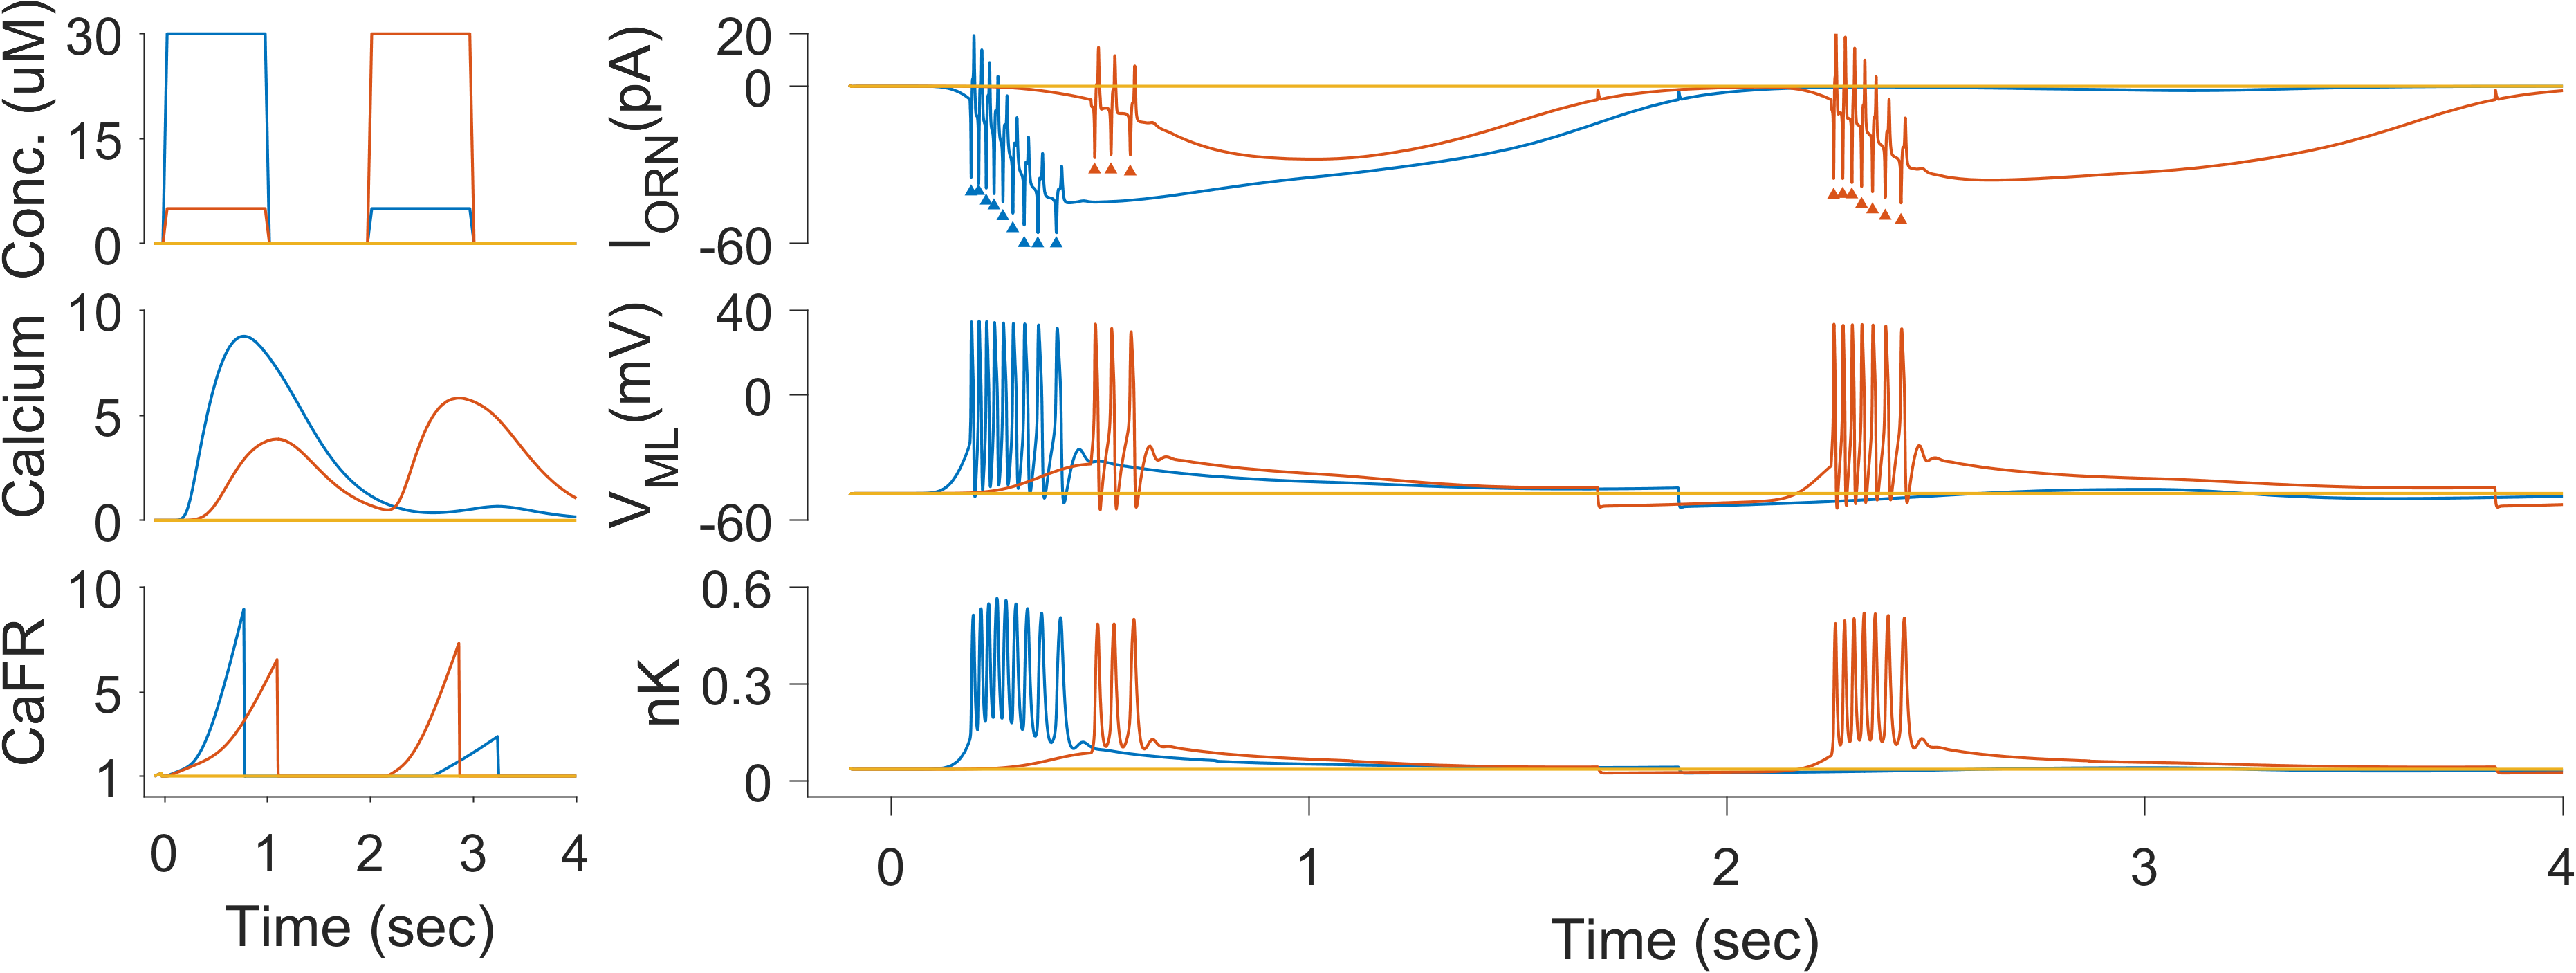
\includegraphics[width=0.9\linewidth]{figs/v1/fig_spk_all_components} 

}

\caption{Spiking ORN operation and key underlying component traces}\label{fig:rORN}
\end{figure}

\hypertarget{response-to-the-stimulus-concentration}{%
\subsubsection{Response to the stimulus concentration}\label{response-to-the-stimulus-concentration}}

\begin{figure}

{\centering \subfloat[Cell current raw traces\label{fig:rCon-1}]{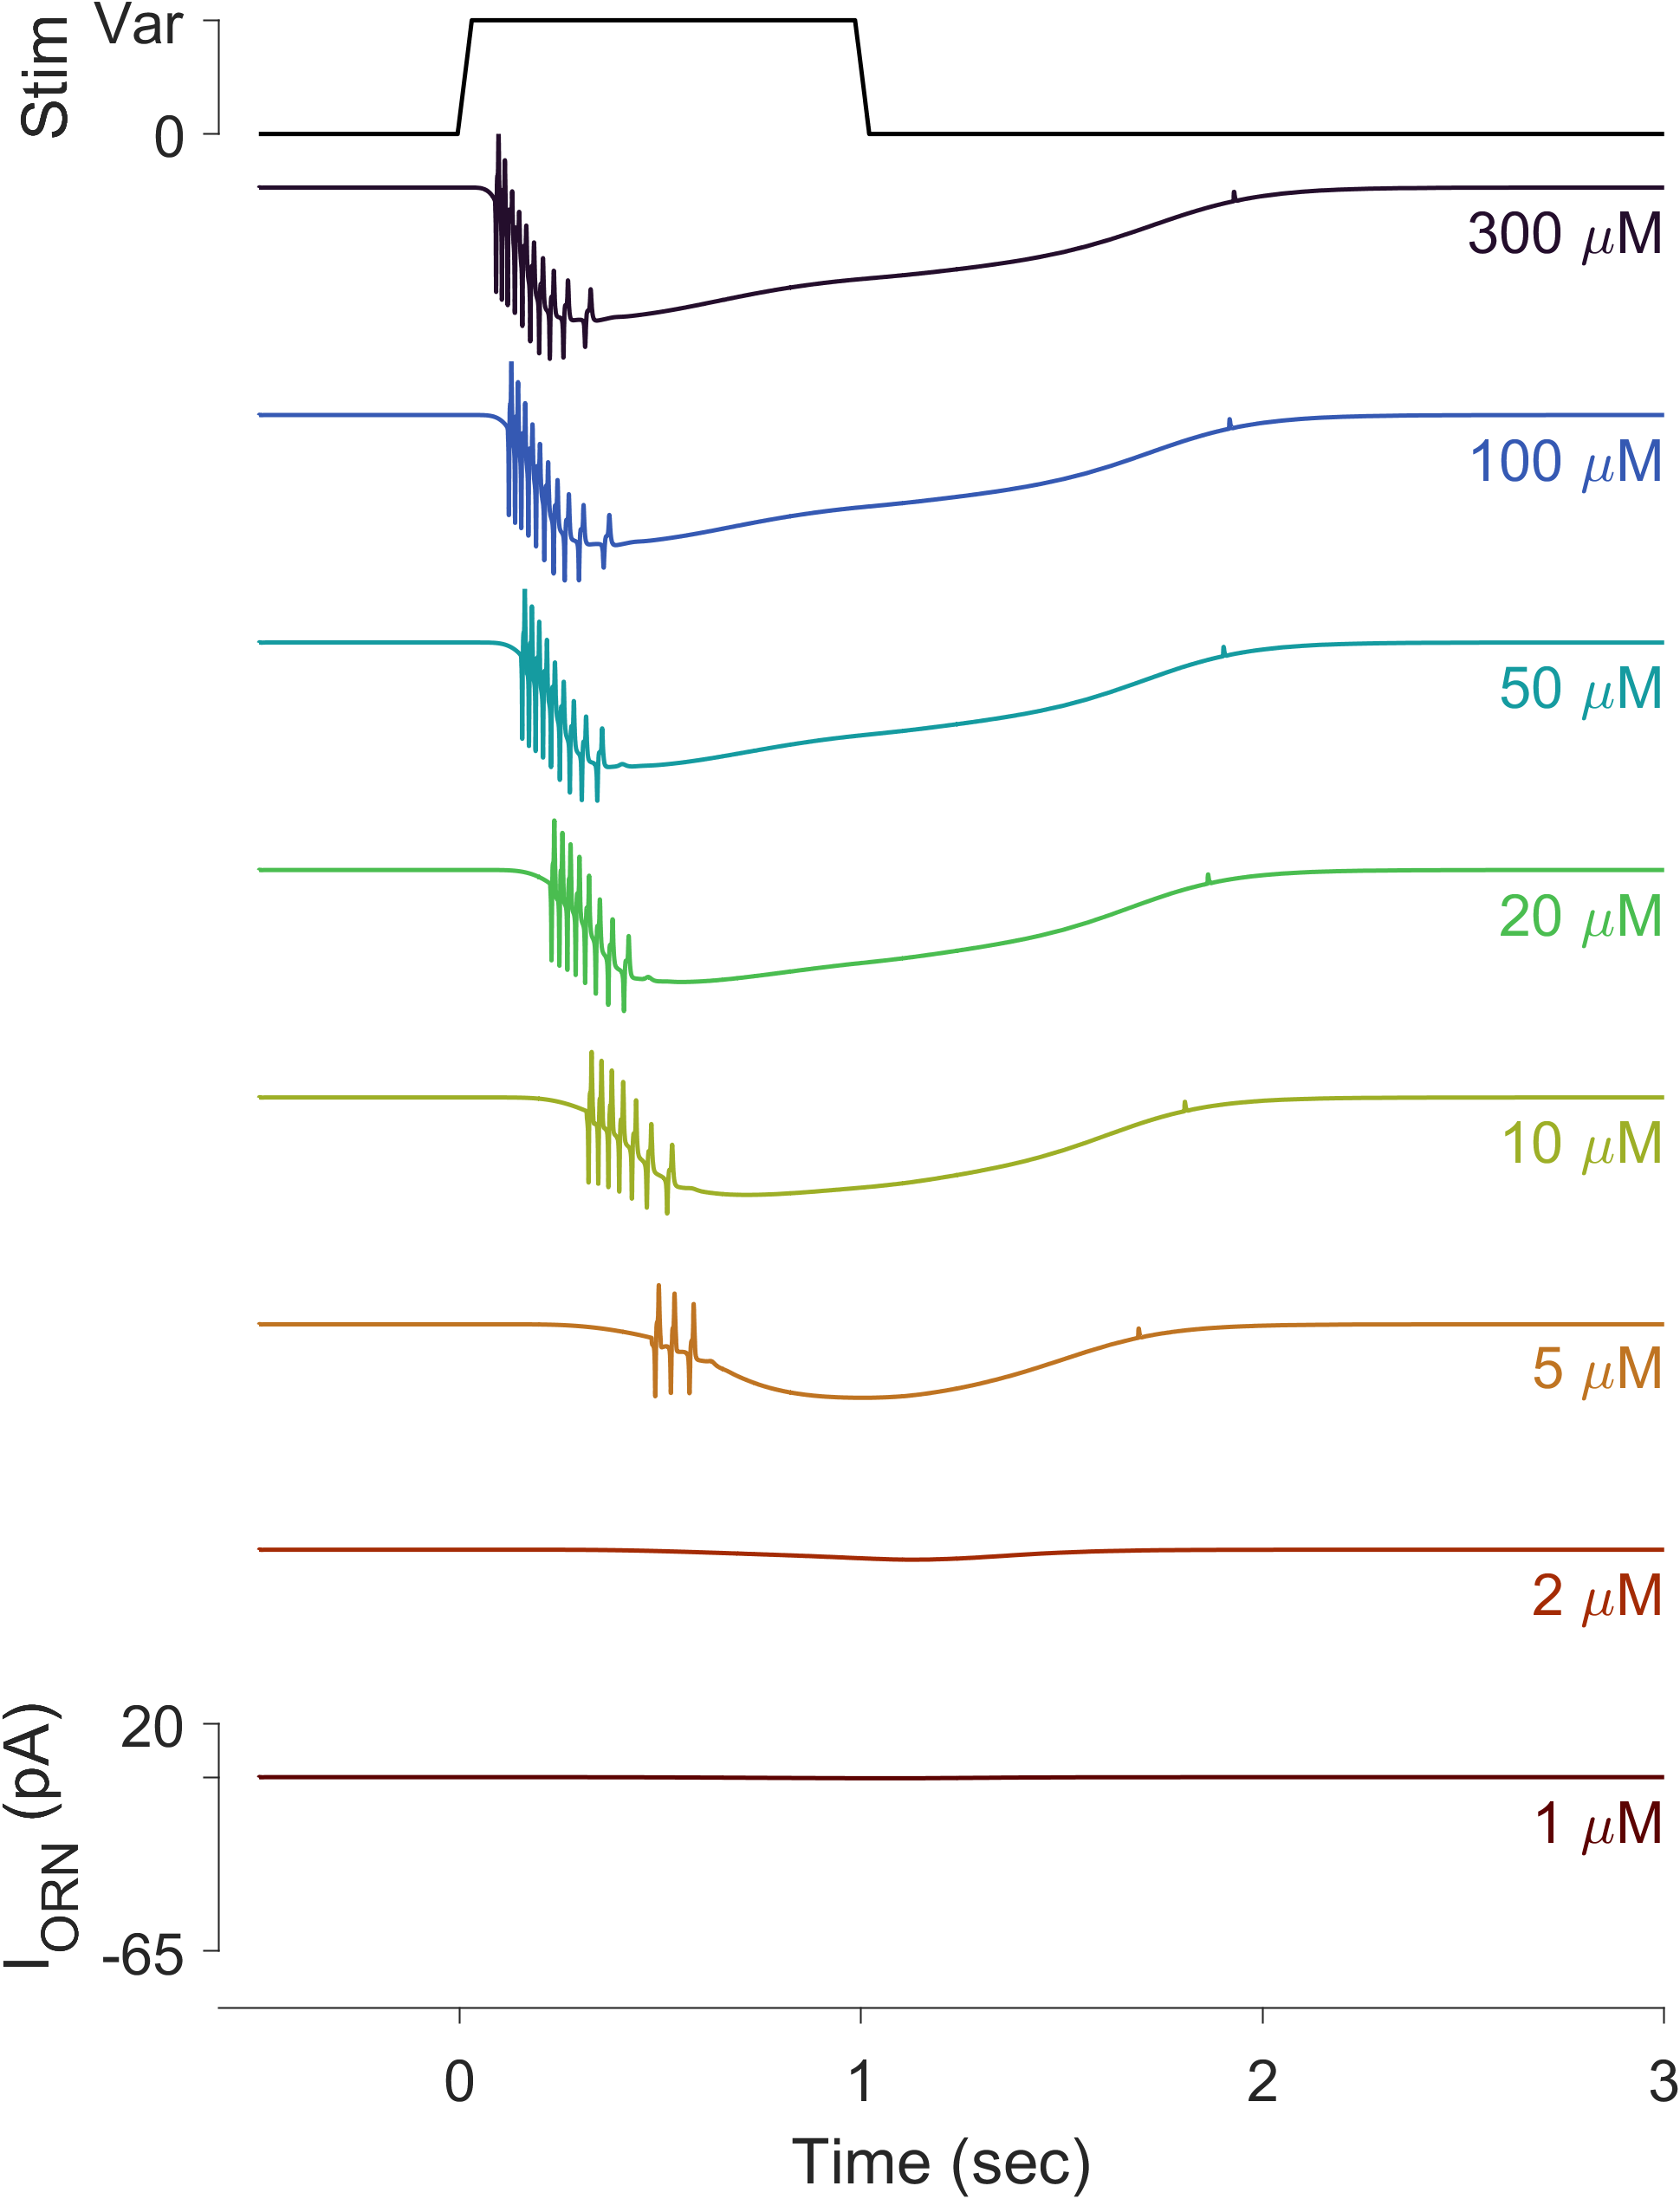
\includegraphics[width=0.5\linewidth]{figs/v1/fig_spk_compare_conc} }\subfloat[Quantification\label{fig:rCon-2}]{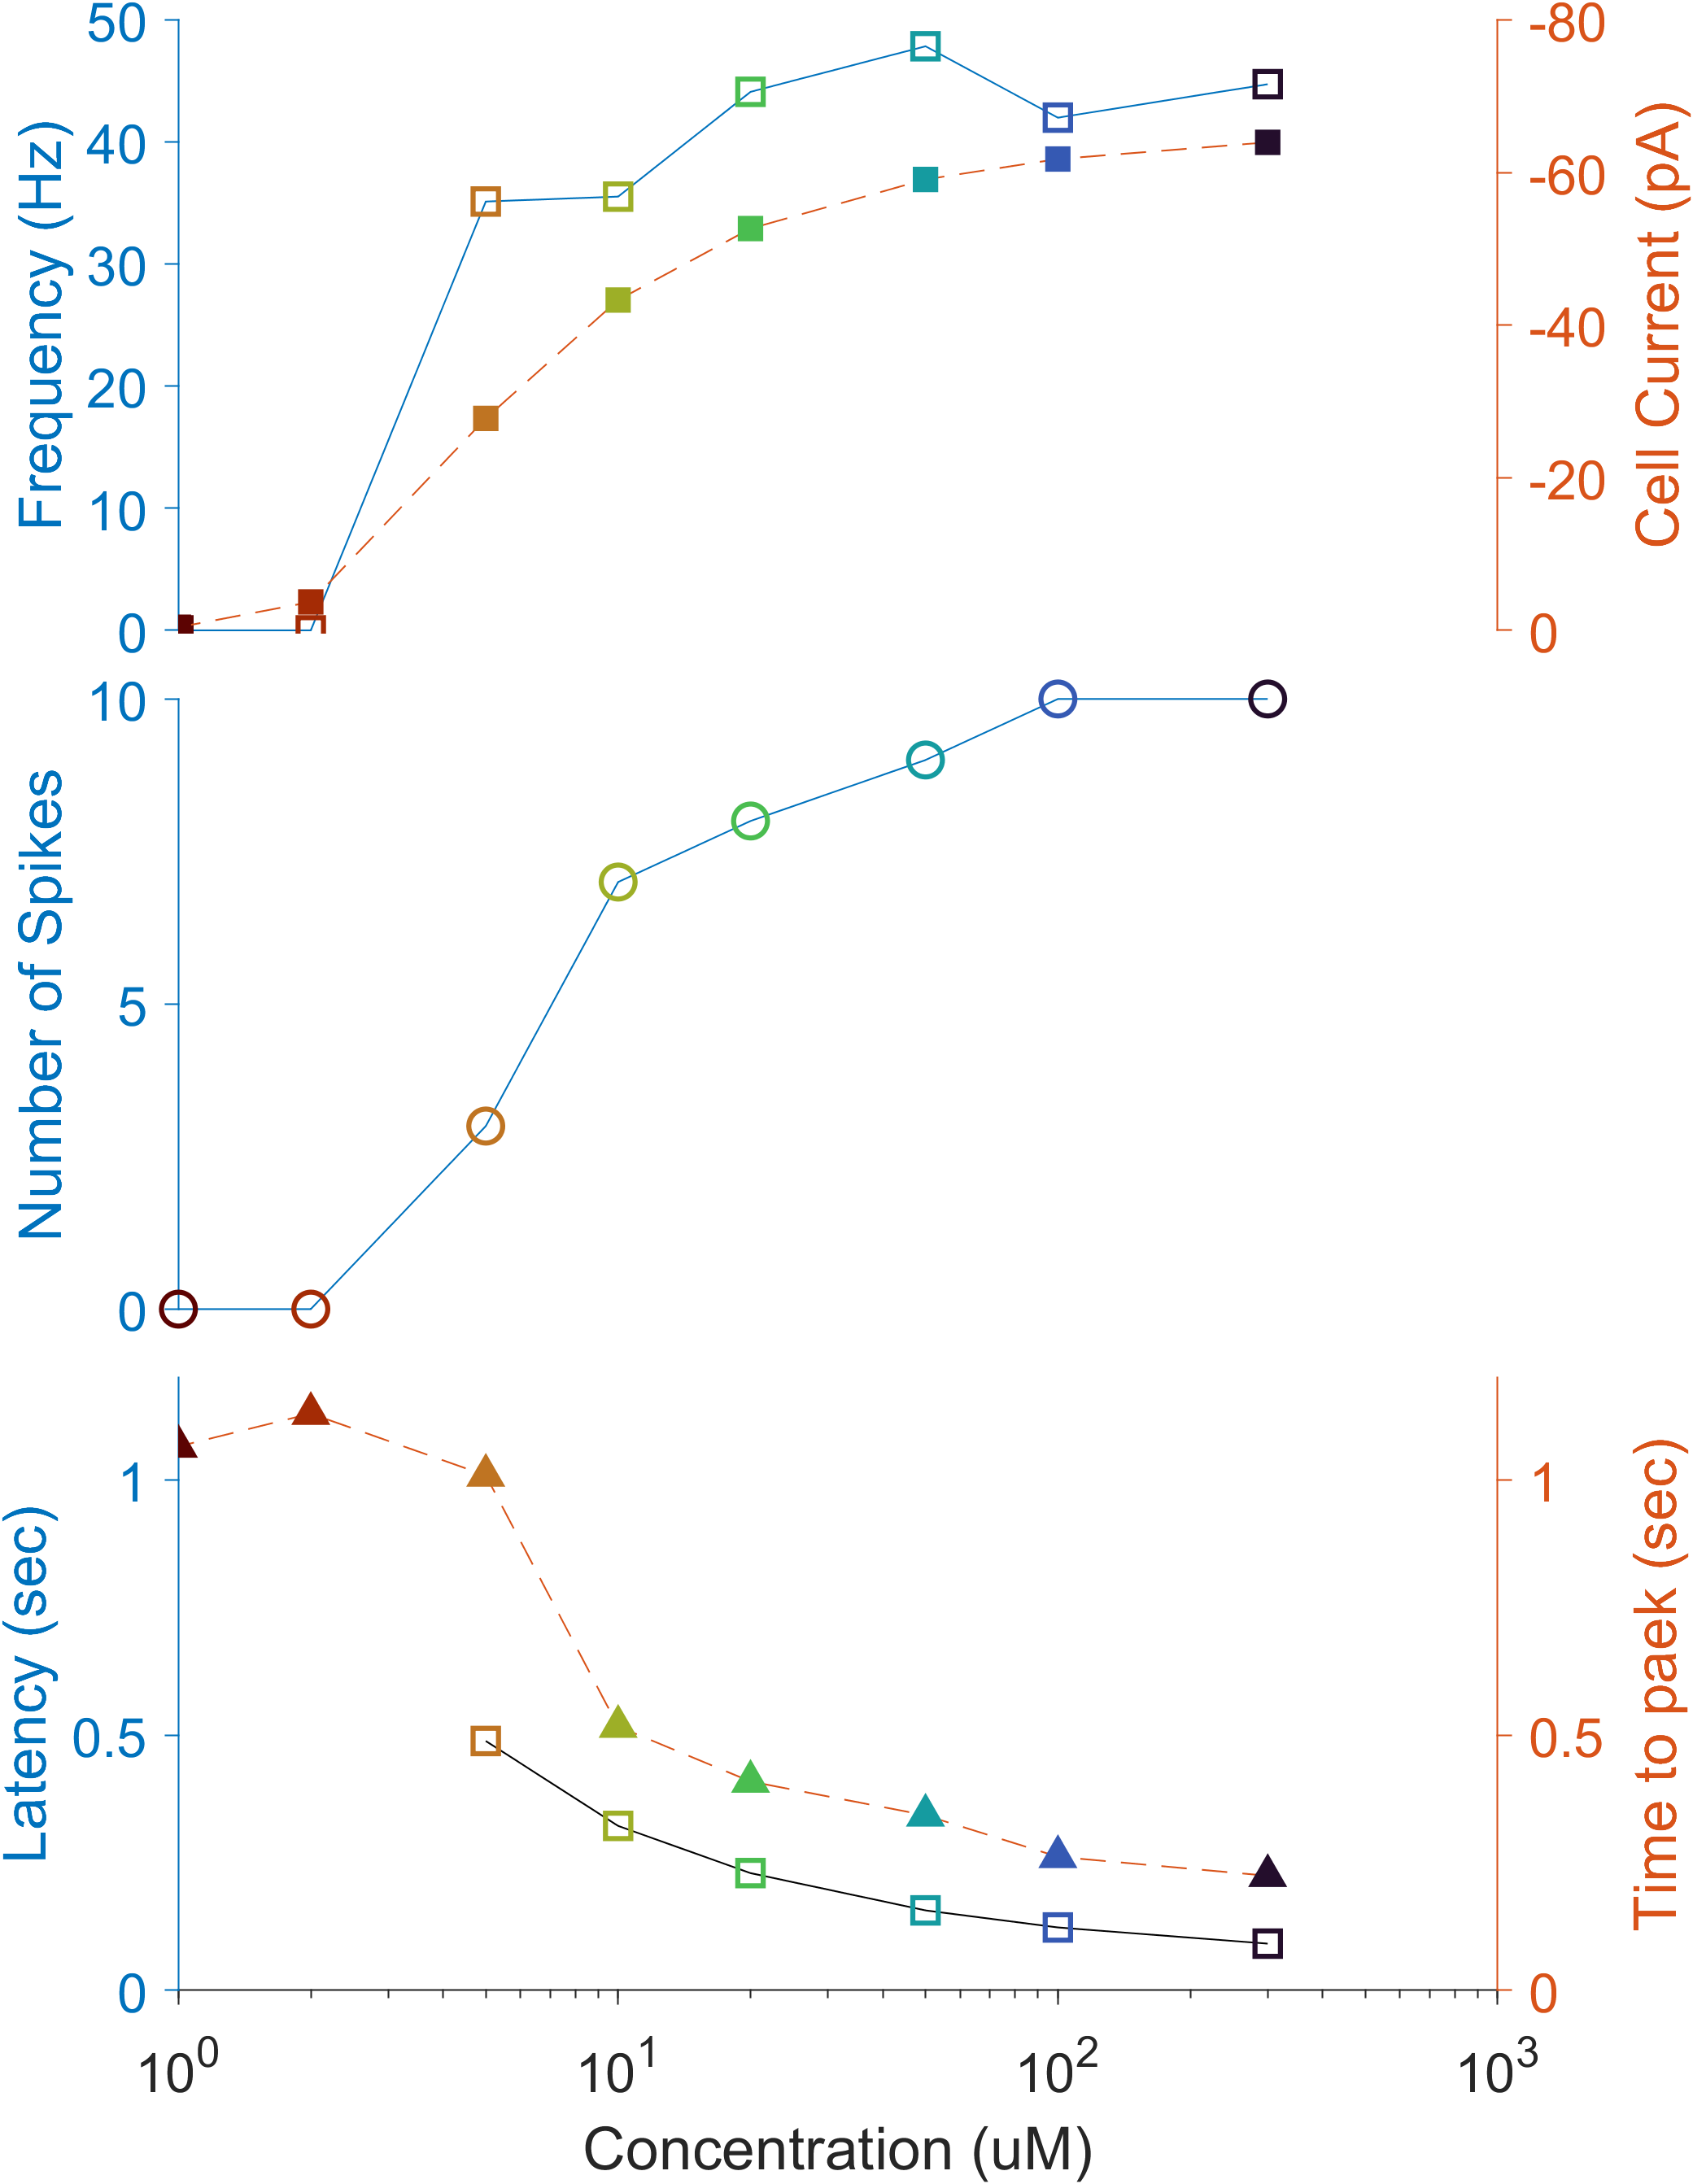
\includegraphics[width=0.5\linewidth]{figs/v1/fig_spk_compare_conc_quant} }

}

\caption{Resulting spiking ORN for different concentrations}\label{fig:rCon}
\end{figure}

Figure-\ref{fig:rCon}(a) shows simulation traces of spiking ORN's response for varying concentration stimulus pulses. Spike-rate, spike-count and latency to the first spike is quantified in (b) for various concentrations and can be used for ORN Spike-response profiling. With increasing stimulus strength, firing-rate and spike-count increases and latency decreases before reaching to the steady-state value. (Experimental data in Fig-\ref{fig:r99f13})

\hypertarget{response-to-the-stimulus-duration}{%
\subsubsection{Response to the stimulus duration}\label{response-to-the-stimulus-duration}}

\begin{figure}

{\centering \subfloat[Transduction-only\label{fig:rDur-1}]{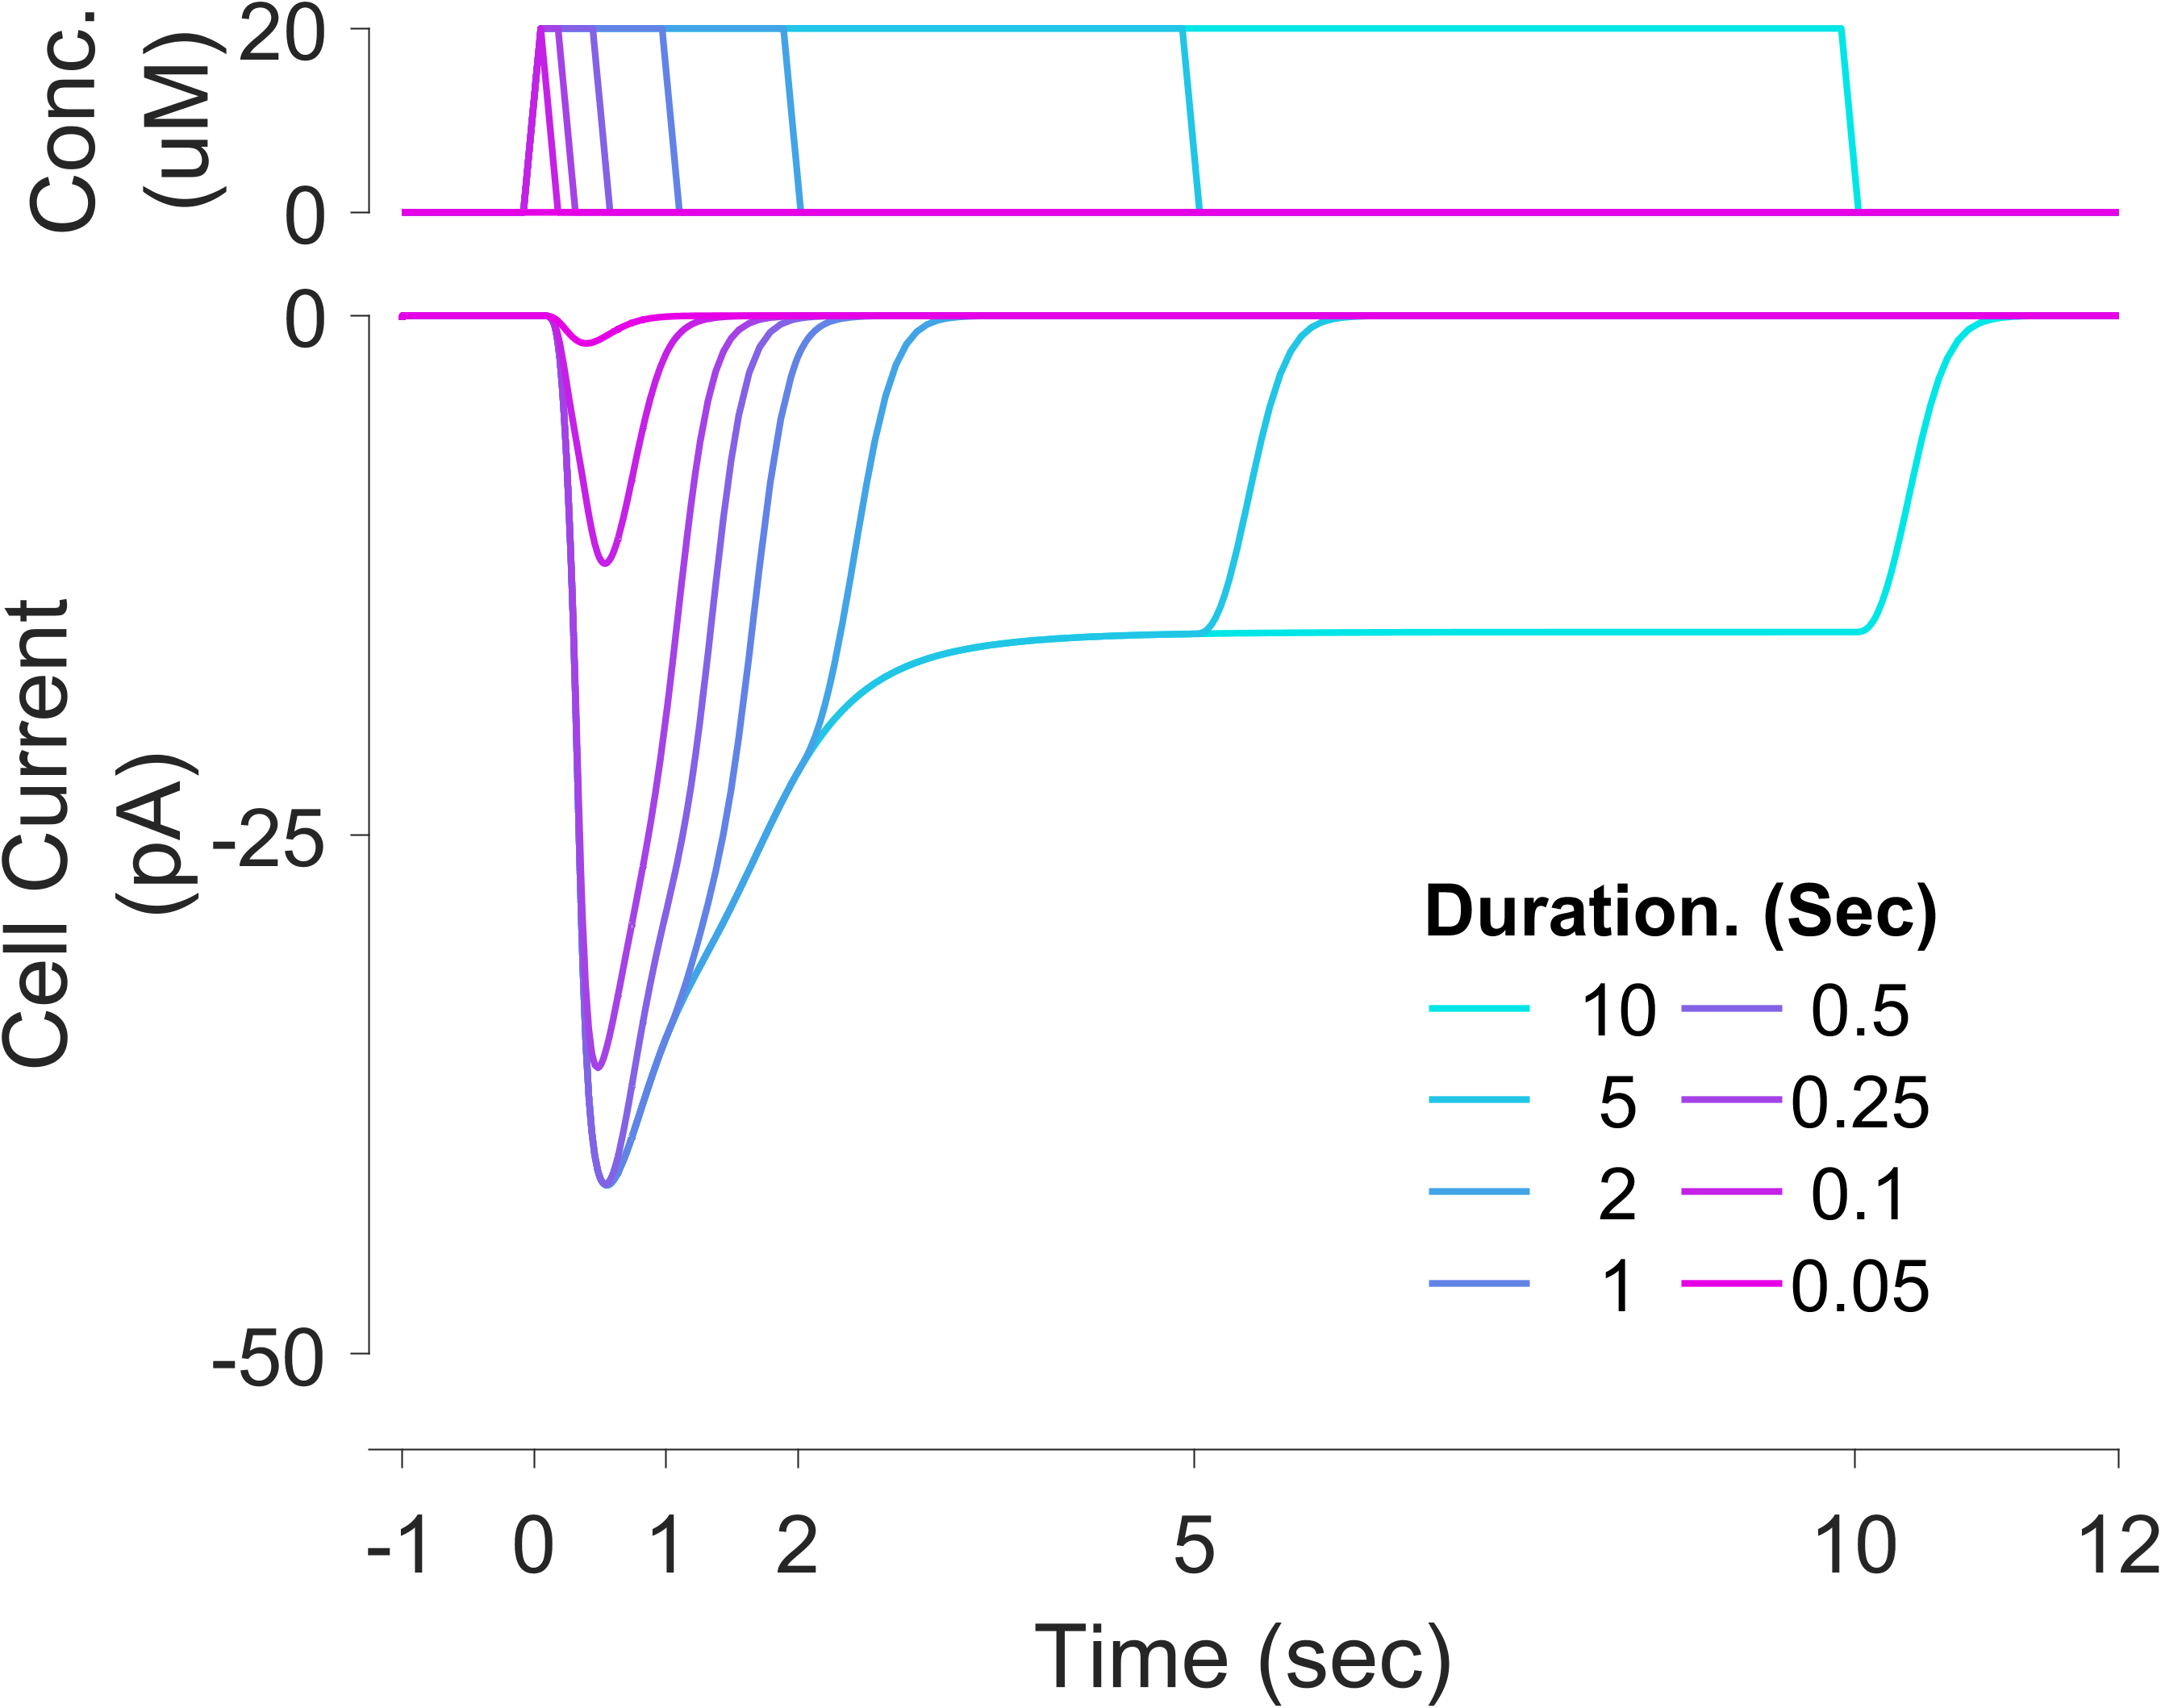
\includegraphics[width=0.5\linewidth]{figs/v1/fig_txn_compare_dur} }\subfloat[Spiking ORN\label{fig:rDur-2}]{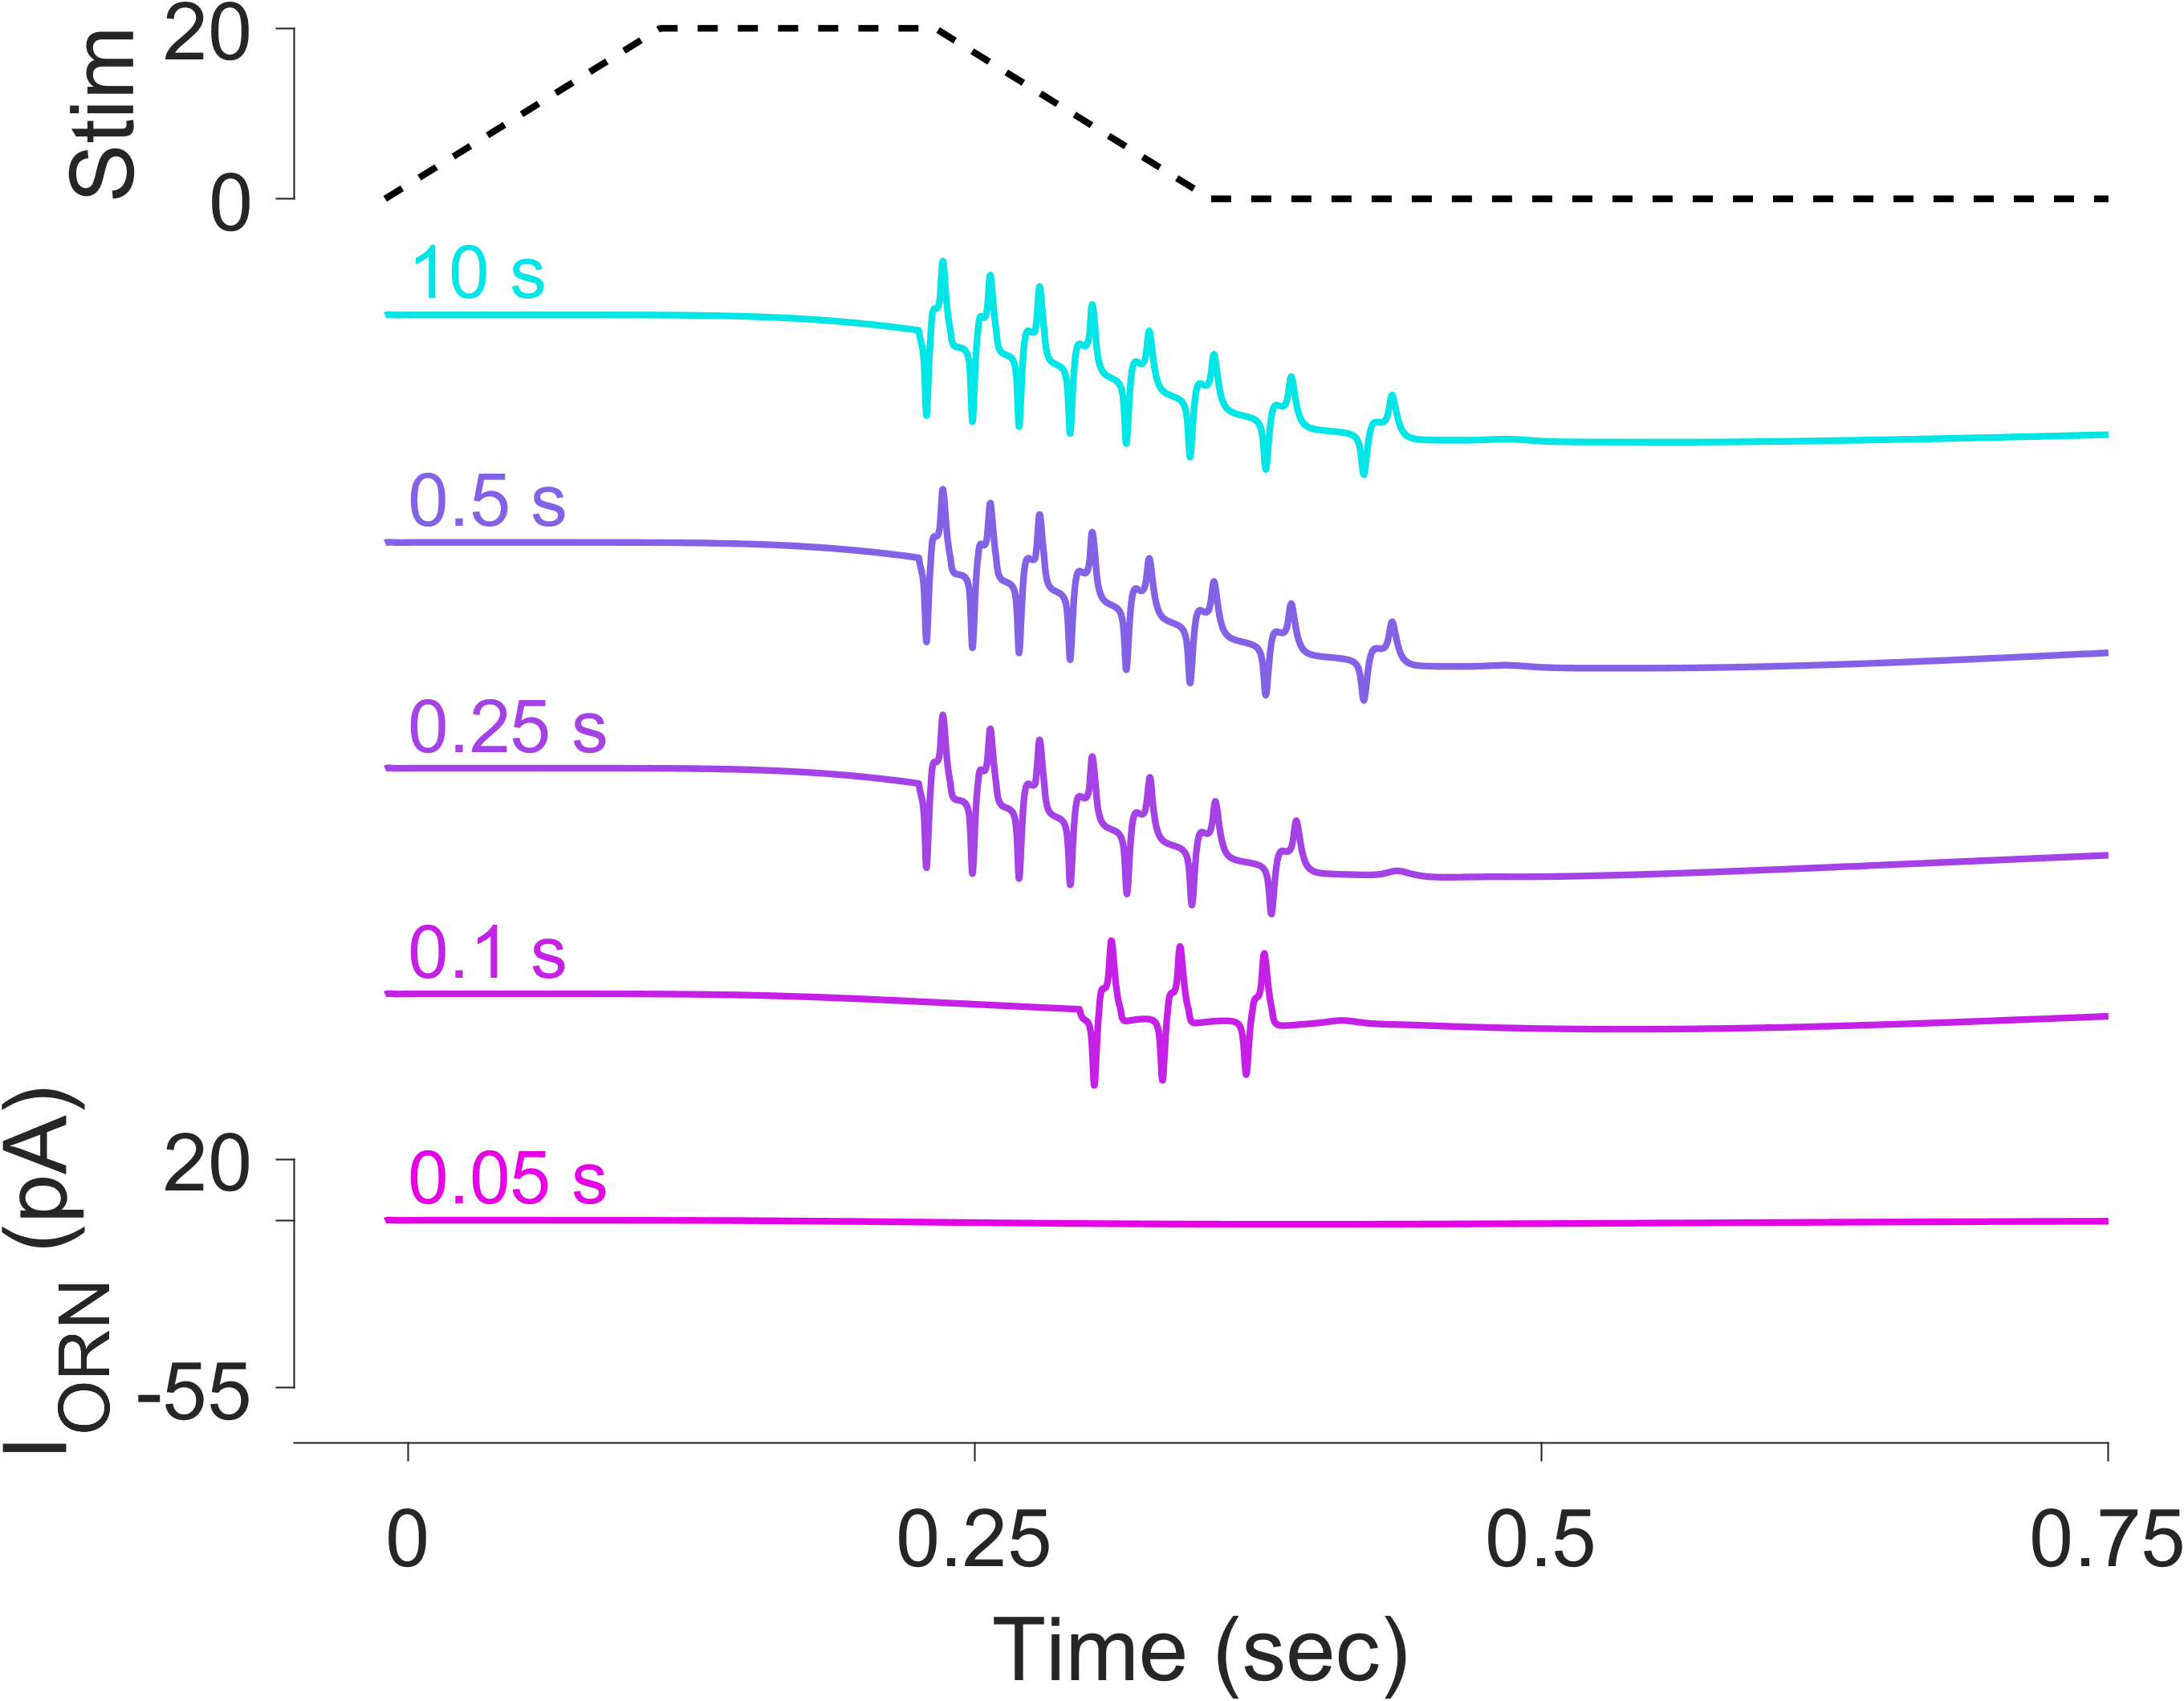
\includegraphics[width=0.5\linewidth]{figs/v1/fig_spk_compare_dur} }

}

\caption{Spiking ORN response for various stimulus duration}\label{fig:rDur}
\end{figure}

Figure-\ref{fig:rDur} shows ORN-transduction and spiking for a single 20 uM stimulus with a varied amount of lengths. As short as 0.1 second stimulus is sufficient to generate spikes in ORN, with an increased latency. Stimulus of 0.5 seconds or longer shows same response in terms of peak transduction current (\ref{fig:rDur}-a), spike-count, spike-frequency and latency (\ref{fig:rDur}-b).

\clearpage

\hypertarget{orn-adaptation-and-spike-response}{%
\subsubsection{ORN adaptation and spike-response}\label{orn-adaptation-and-spike-response}}

To find the effect of adaptation and to compare it with experimental data shown in fig-\ref{fig:r99f5}, I stimulated the spiking ORN with a 4 second pre-stimulus pulse of variable concentrations followed by an 1 second long test pulse of 20 uM odor concentration. Figure-\ref{fig:rAdp} shows the result which matches the experimental data. A pre-stimulus of 2 uM or stronger does not yield any spikes for the test-stimulus, though they show transduction response for the test-pulse. Spike counts get reduced with increasing concentration of pre-stimulus.

\begin{figure}

{\centering 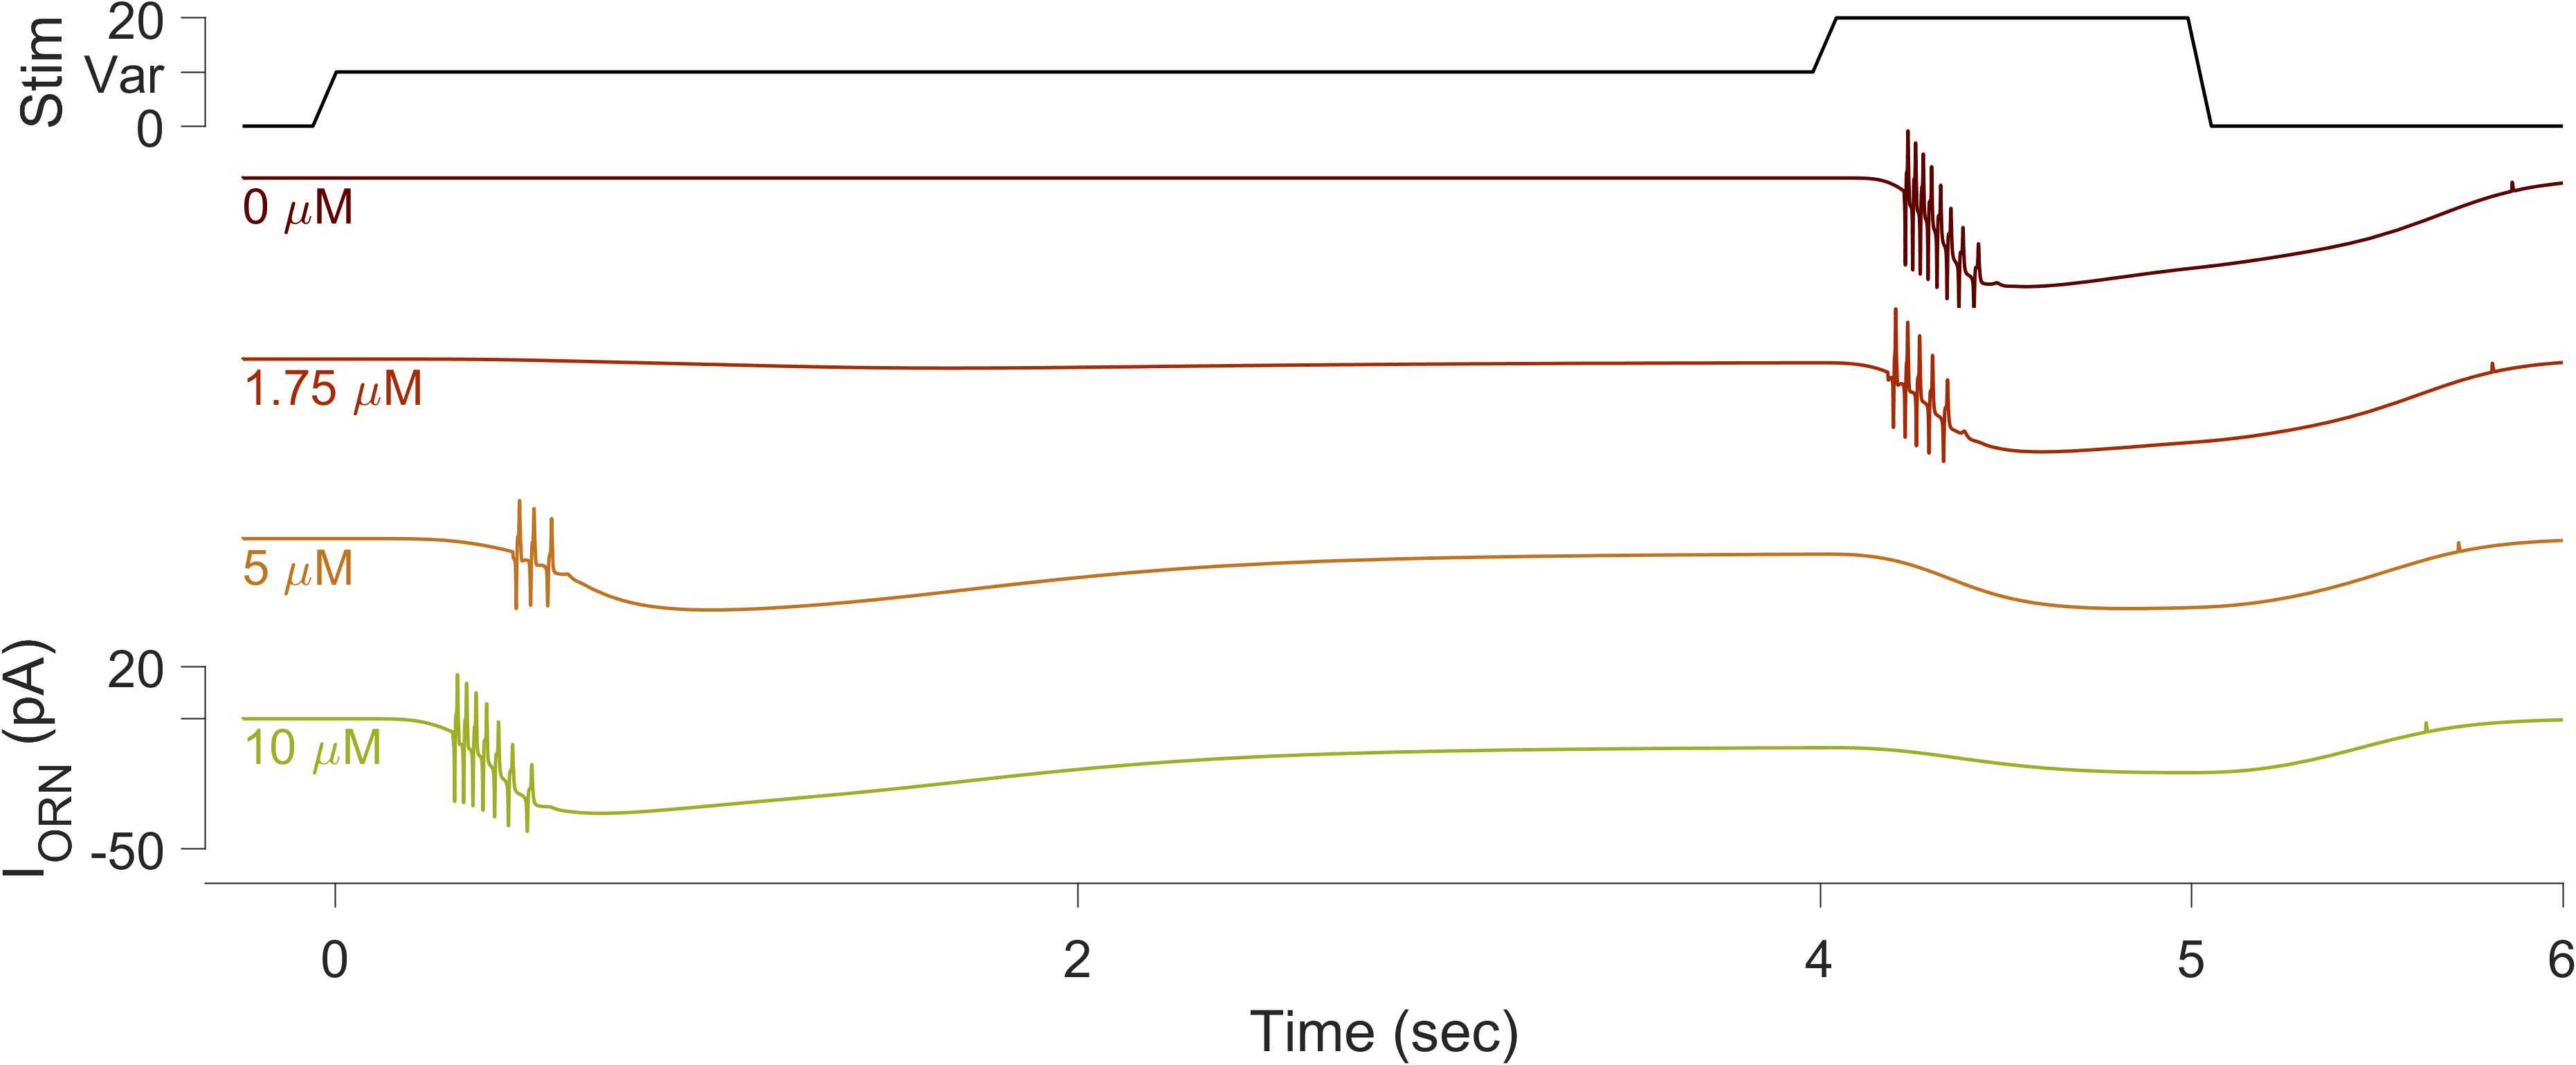
\includegraphics[width=0.9\linewidth]{figs/v1/fig_spk_compare_adaptation} 

}

\caption{Effect of adaptation on ORN spiking response}\label{fig:rAdp}
\end{figure}

\hypertarget{sniffing-experiment-1}{%
\subsection{Sniffing experiment}\label{sniffing-experiment-1}}

A hypothesis I am testing testing for the sniffing experiment is the following :

\begin{quote}
A higher breathing frequency will have higher adaptation and, hence, a lower steady-state response in ORN.
\end{quote}

\begin{figure}

{\centering 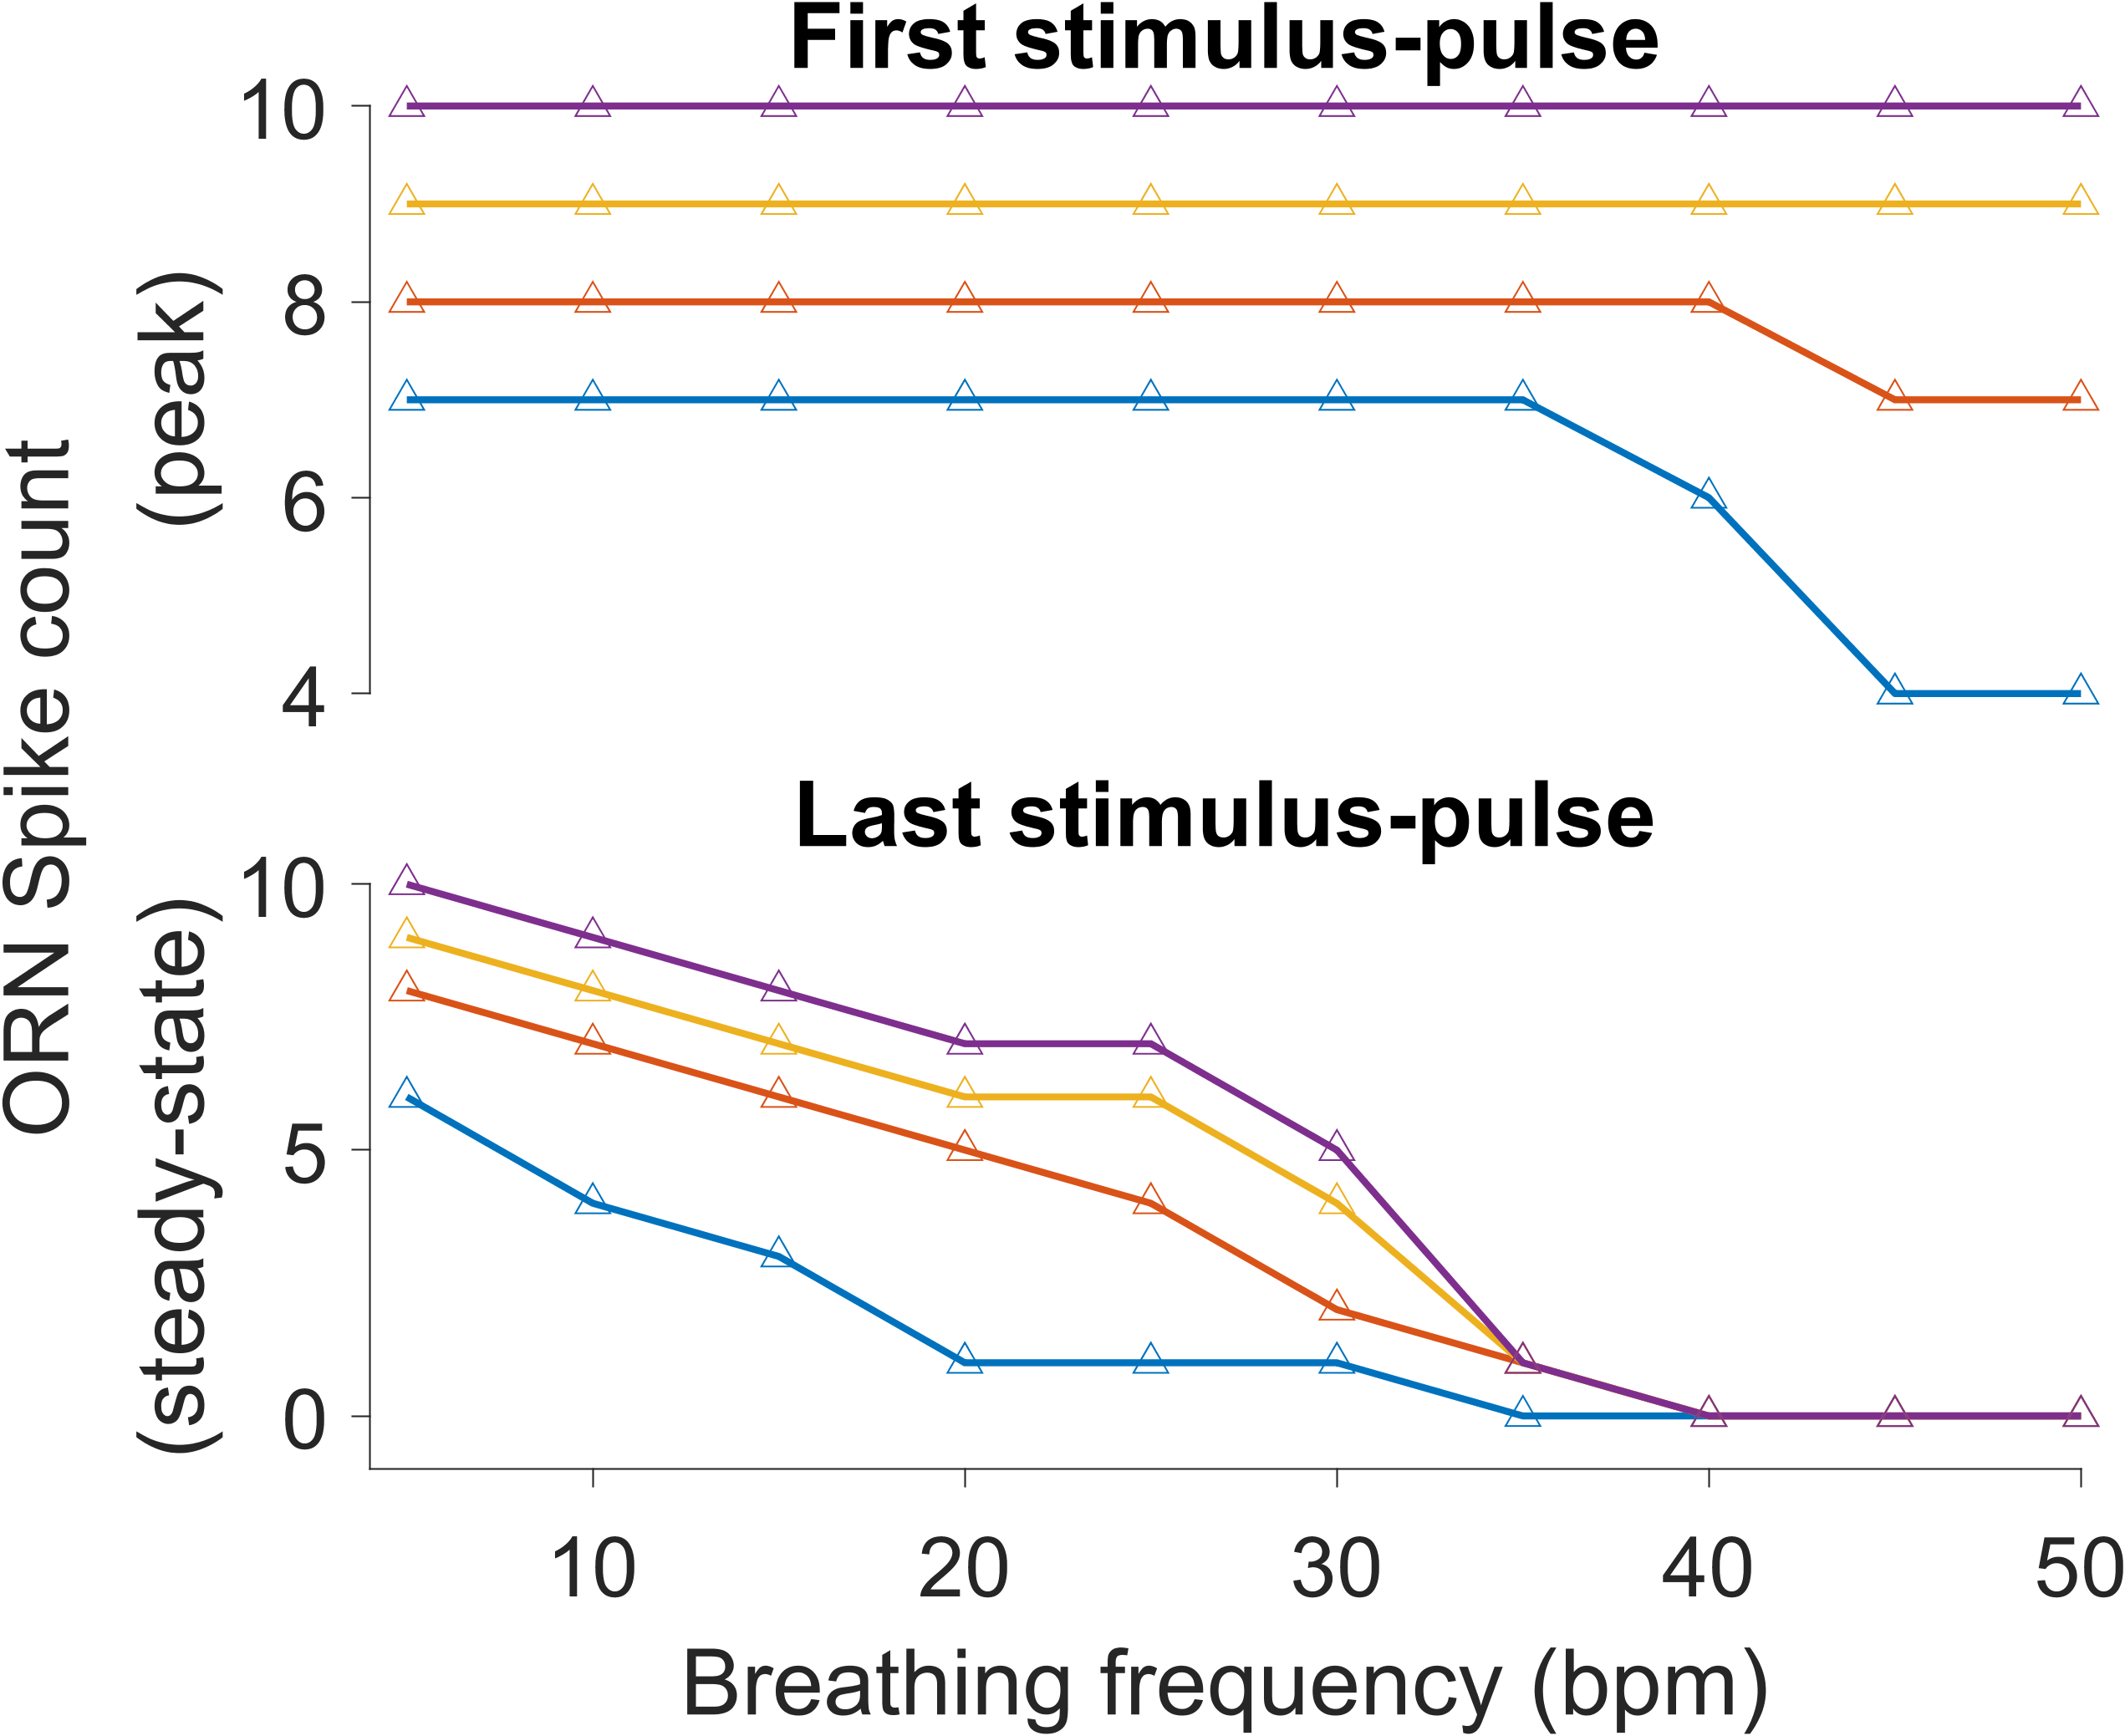
\includegraphics[width=0.5\linewidth]{figs/v1/fig_sniff_freq_FR_tuning_raw} 

}

\caption{Spike counts for various breathing rate (breaths/min)}\label{fig:rSen1}
\end{figure}

To address this question, I am quantifying peak and steady-state spike-response using the spike-count as the ORN response indicator. Figure-\ref{fig:rSen1} shows number of spikes during the first-sniff (peak-count) vs the last-sniff (steady-state). The steady-state spike counts steadily decrease with increasing breathing frequency, which supports the hypothesis.

\hypertarget{optimal-sniffing-frequency}{%
\subsubsection{Optimal sniffing frequency}\label{optimal-sniffing-frequency}}

The optimal frequency would the highest breathing frequency with little loss of ORN sensitivity. See \(\S\)\ref{CD}(F) for the discussion over defining ORN sensitivity.

\begin{figure}

{\centering 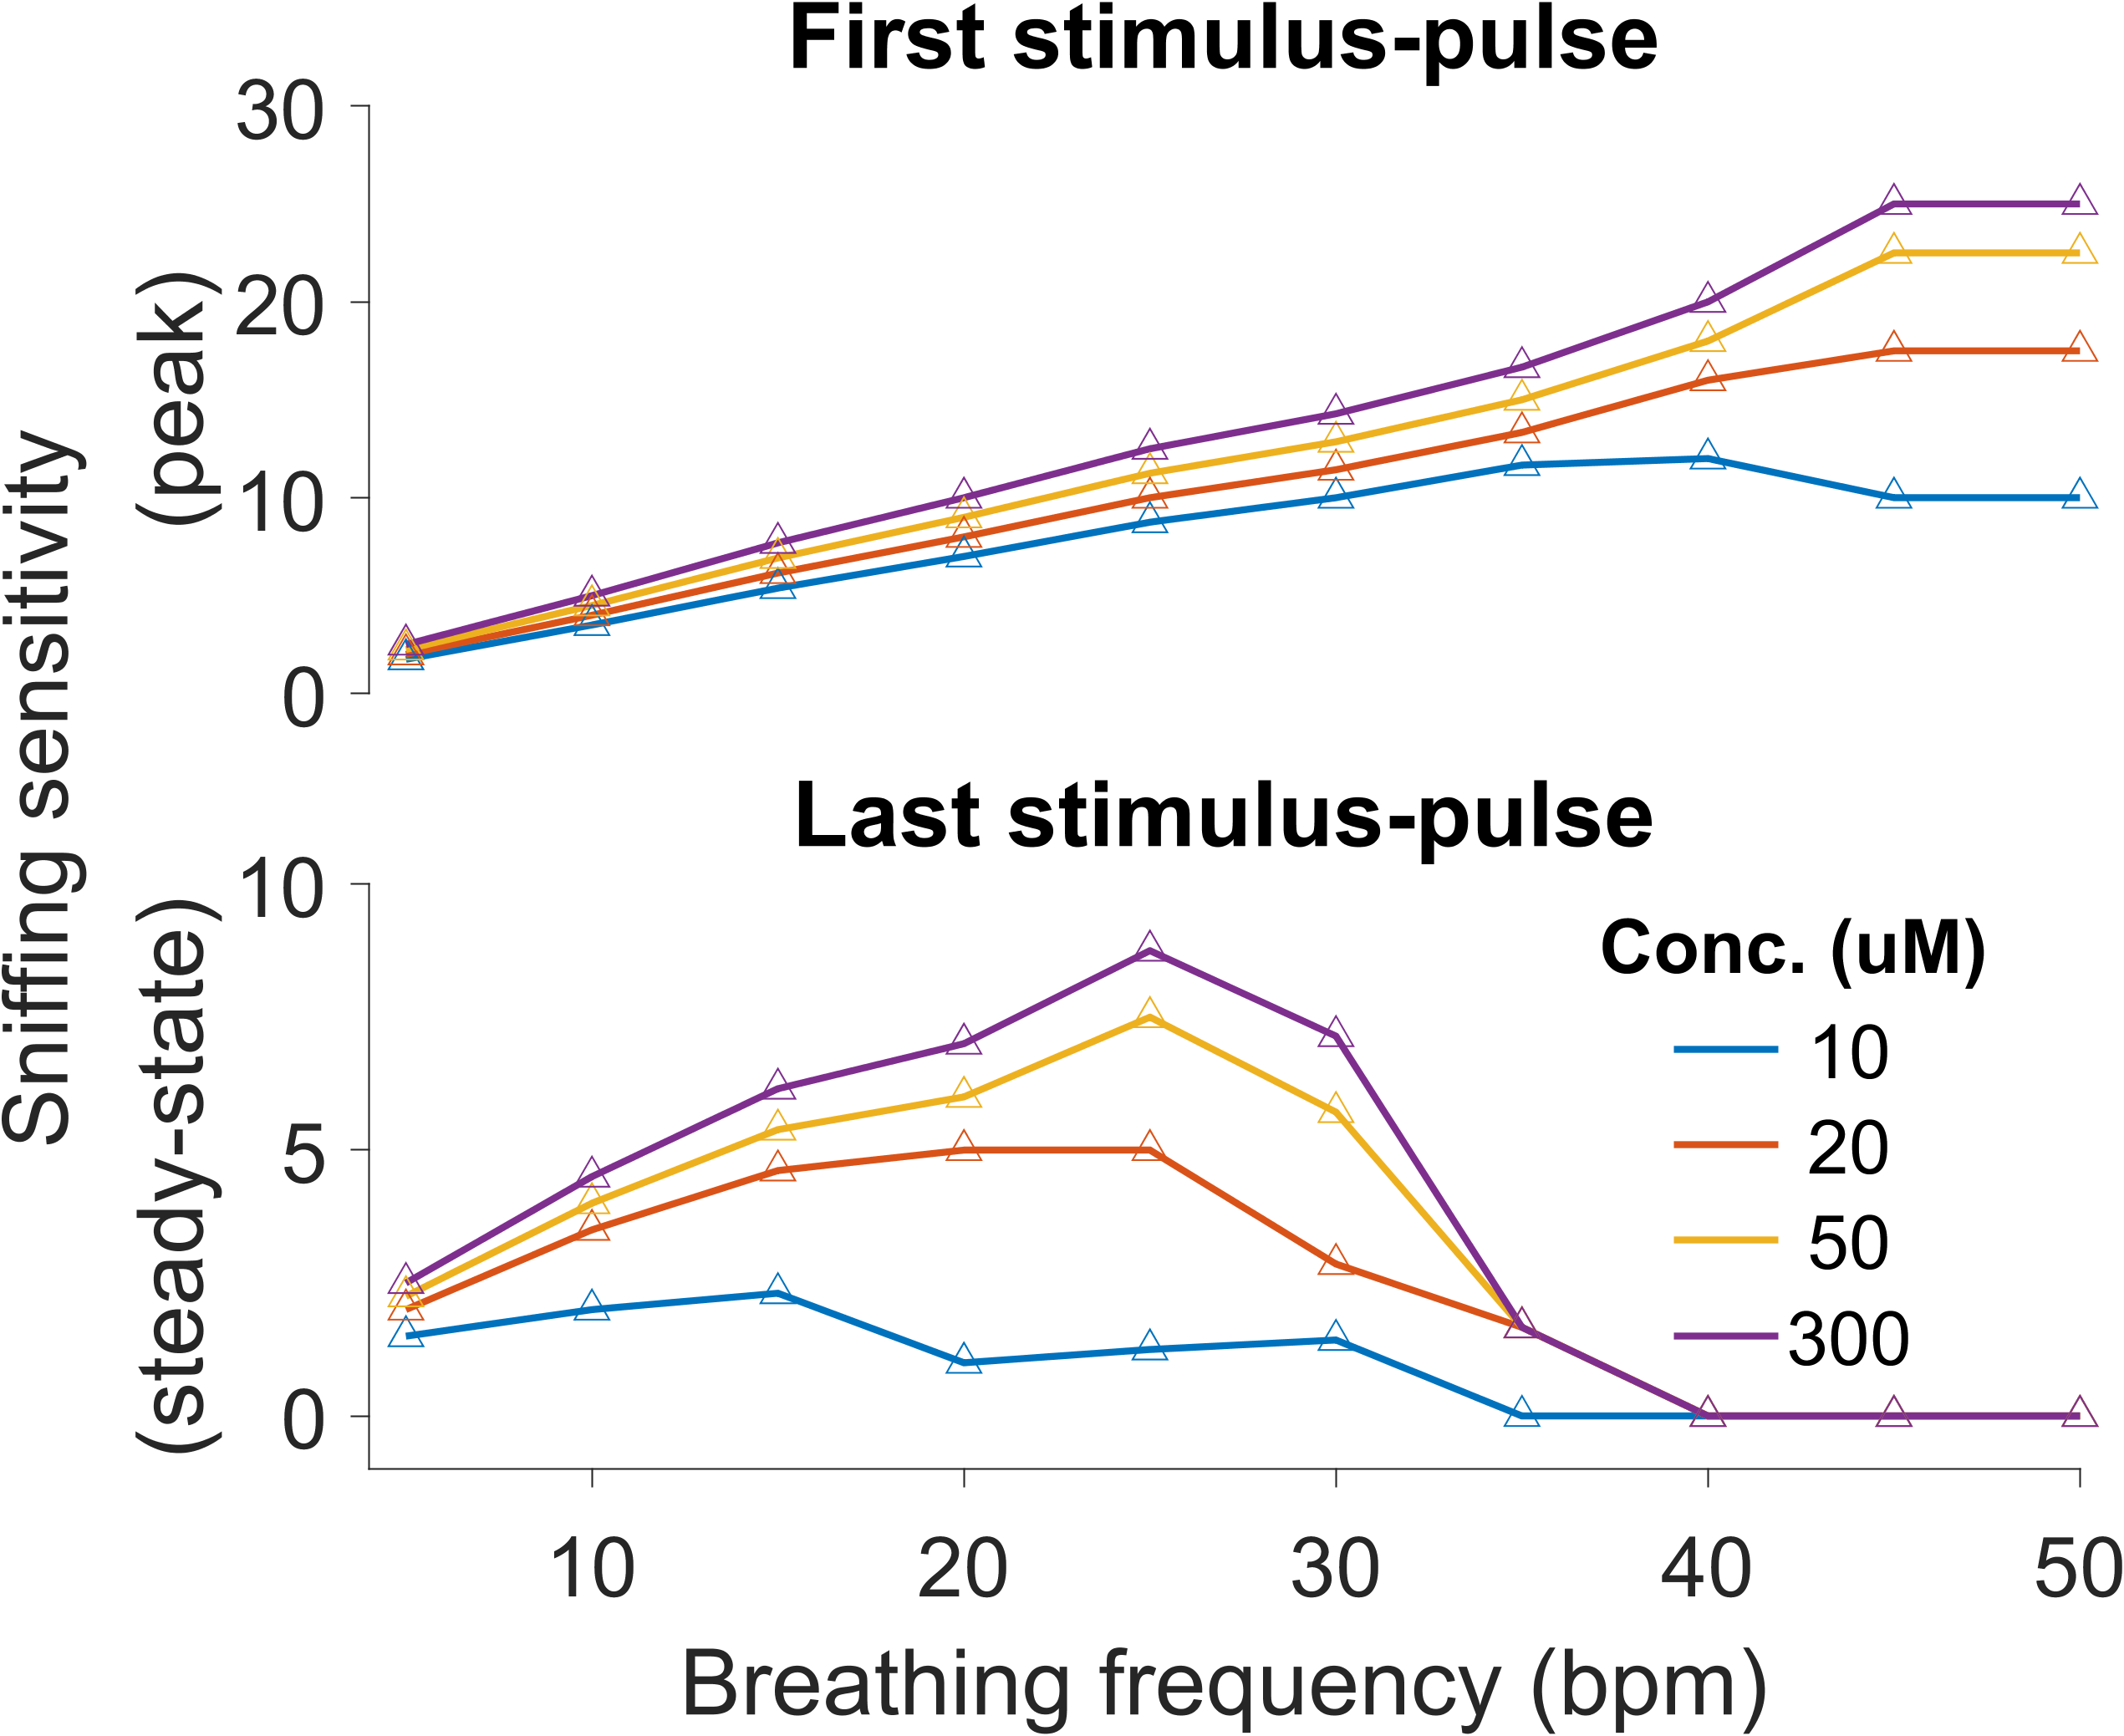
\includegraphics[width=0.5\linewidth]{figs/v1/fig_sniff_freq_FR_tuning_gain} 

}

\caption{ORN sensitivity for various breathing rate (breaths/min)}\label{fig:rSen2}
\end{figure}

Figure-\ref{fig:rSen2} shows peak and steady-state sniffing sensitivity for various breathing frequencies. The range between 25 to 30 breaths/min shows optimal sniffing sensitivity.

Raw traces for the data-points in Figure-\ref{fig:rSen1} \& \ref{fig:rSen2} are included in Appendix C.

\hypertarget{CD}{%
\section{Discussion and Conclusion}\label{CD}}

\begin{enumerate}
\def\labelenumi{\Alph{enumi}.}
\tightlist
\item
  \textbf{Transduction simulation matches experimental data in terms of the response-shape but show a smaller peak current response}
\end{enumerate}

Peak cellular current in ORN transduction simulation (Fig-\ref{fig:txCon},\ref{fig:txAdp}) is lower in amplitude as compared to the experimental data (Fig-\ref{fig:r99f24}). However, both matches in overall shape and trends. This difference is inherited from the ORN model I used from the previous study (Dougherty, Wright, and Yew 2005). It provided multiple sets of fitted parameters for the ORN transduction model and I have used the set suitable for Ca-based adaptation simulation. Since my goal of this study was to introduce action potentials in ORN, I did not try to match the peak current. One can use the parameters optimized for ORN concentration response (Dougherty 2005) or modify the transduction model for matching peak-currents. Hence, I am disregarding the current scales of the spike-response simulations while matching to the raw data.

\begin{enumerate}
\def\labelenumi{\Alph{enumi}.}
\setcounter{enumi}{1}
\tightlist
\item
  \textbf{Morris-Lecar (ML) model can be integrated in mechanistic ORN model and it is different than just adding ML spikes post-simulation}
\end{enumerate}

\S\ref{ML} shows the method I used to introduce ML spikes in ORN simulations, which uses three additional ODEs integrated along with others from sensory-transduction in mutually dependent fashion. Meaning, change in ML voltage will alter species concentrations of transduction mechanisms and vice versa. Just to demonstrate how ML spikes in an ORN would look if they were added later after the transduction simulation, see Figure-\ref{fig:MLover}, which does not look realistic or match to the raw data. Hence, I have integrated ML processes along with the molecular transduction processes for my spiking ORN model to simulate realistic ORN current signals.

\begin{enumerate}
\def\labelenumi{\Alph{enumi}.}
\setcounter{enumi}{2}
\tightlist
\item
  \textbf{Spike identification works robustly for both low and high concentrations}
\end{enumerate}

Figure-\ref{fig:MLspkID} shows spike identified in a lower and higher concentration stimulus. I did not use a threshold based method to identify the spikes but used an algorithm to find local minima in ML spikes. Primary purpose to identify spikes in ORN is to use them in stimulus-response profiling shown in Figure-\ref{fig:rCon} and \ref{fig:rSen1}. Another example for robustness of spike-identification can be seen in plots in Appendix C, and especially in steady-state response (Fig-\ref{fig:f10bpmSS}).

\begin{enumerate}
\def\labelenumi{\Alph{enumi}.}
\setcounter{enumi}{3}
\tightlist
\item
  \textbf{\texttt{CaFR} can modulate firing frequency dynamically to match experimental data}
\end{enumerate}

Without \texttt{CaFR} (i.e.~\({\rm CaFR}=1\) and \(\dot{\rm CaFR}=0\)) we will get a fixed firing frequency of ORN spikes (see Fig-\ref{fig:aCaFR1}). However, \texttt{CaFR} causes high spike-rate at the beginning of the stimulus and reducing over time to match the firing trend found in experimental data (Appendix A). Though, \texttt{CaFR} is a mathematical phenomenon, it matches the operation of certain recently found calcium-activated chloride channels which inhibit the cell and clamp the ORN firing activity (Zak et al. 2018). However, \texttt{CaFR} does not modulate the period in which cell is firing. That is determined by the intracellular calcium (value readout from the transduction process) dependent current, \(I_{\rm Ca}\), used in the ML spikes model.

\begin{enumerate}
\def\labelenumi{\Alph{enumi}.}
\setcounter{enumi}{4}
\tightlist
\item
  \textbf{ML spikes in ORN model matches to high concentration responses in experimental data but not to the lower concentrations due to mismatching spike-counts}
\end{enumerate}

ORN spikes in Figure-\ref{fig:rCon} and \ref{fig:rAdp} matches the experimental data Figure-\ref{fig:r99f13}-\ref{fig:r99f5} in terms of latency and spike frequency. For my model, spike frequency is modeled after slope of calcium-intake, which reduces spike-counts for lower slope and inhibits in negative slope. This prevents my spiking ORN model to have the sustained spikes seen in Figure-\ref{fig:r99f5} as a response of a prolong low-concentration stimulus. This also explains lack of very high spike-counts for lower concentrations as seen in Figure-\ref{fig:r99f13}(b). Such response can be matched likely by adding a separate dynamics activated based on something like \texttt{aG} and inhibited by \texttt{Ca}. I did not add them here as my aim for this study was to match initial spike response of ORN in response of stimulus-concentration and adaptation, and not the modeling of baseline ORN firing.

\begin{enumerate}
\def\labelenumi{\Alph{enumi}.}
\setcounter{enumi}{5}
\tightlist
\item
  \textbf{Sniffing sensitivity can identify suitable breathing frequency for frog ORN}
\end{enumerate}

Sniffing sensitivity is defined as the spike count for a given odor-stimulus duration. So, for a same duration stimulus, higher number of spike responses in the ORN will yield higher sensitivity. Also, for the same number of spike responses, a shorter duration odor-stimulus will indicate higher sensitivity. Increasing sensitivity with increased sniffing-frequency is a potential mechanism to optimize olfactory search duration especially in turbulent environments (Baker et al. 2018). Higher sniffing frequency can help detect odor signals in fast-changing environments. Thus, the optimal sniffing frequency should have both the higher breathing rate and higher sniffing sensitivity, in order to navigate efficiently (e.g.~finding an odor-souce quickly) in a turbulent odor environment.

\hypertarget{conclusion}{%
\paragraph*{Conclusion}\label{conclusion}}
\addcontentsline{toc}{paragraph}{Conclusion}

In summary, ML model can be used to represent action potential responses encoded in frog ORNs with certain limitations. The spiking ORN model can be used for adaptation and sniffing related experiments. I found higher adaptation response for a higher breathing frequency in ORN, which is matching to my hypothesis and is consistent with the biological expectations. Such simulations can be used to understand olfactory search strategies and other odor-guided animal behaviors.

\clearpage

\hypertarget{appendix-appendix}{%
\appendix}


\hypertarget{appendix-a-experimental-data-for-comparing-with-simulation}{%
\section*{Appendix A : Experimental data (for comparing with simulation)}\label{appendix-a-experimental-data-for-comparing-with-simulation}}
\addcontentsline{toc}{section}{Appendix A : Experimental data (for comparing with simulation)}

\hypertarget{orn-transduction}{%
\subsection*{ORN transduction}\label{orn-transduction}}
\addcontentsline{toc}{subsection}{ORN transduction}

\begin{figure}

{\centering \subfloat[Reisert, 1999 - Fig-2\label{fig:r99f24-1}]{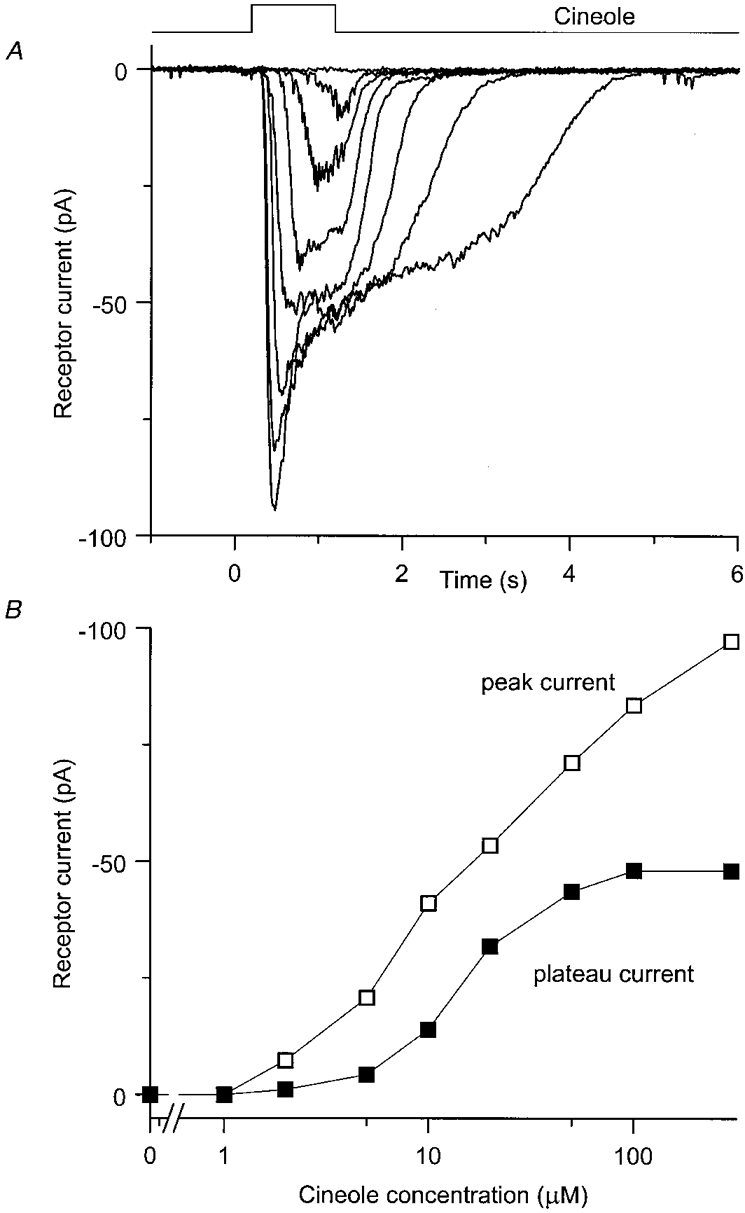
\includegraphics[width=0.5\linewidth]{figs/Reisert1999/fig_txn_compare_conc_quant_R99_F2} }\subfloat[Reisert, 1999 - Fig-4\label{fig:r99f24-2}]{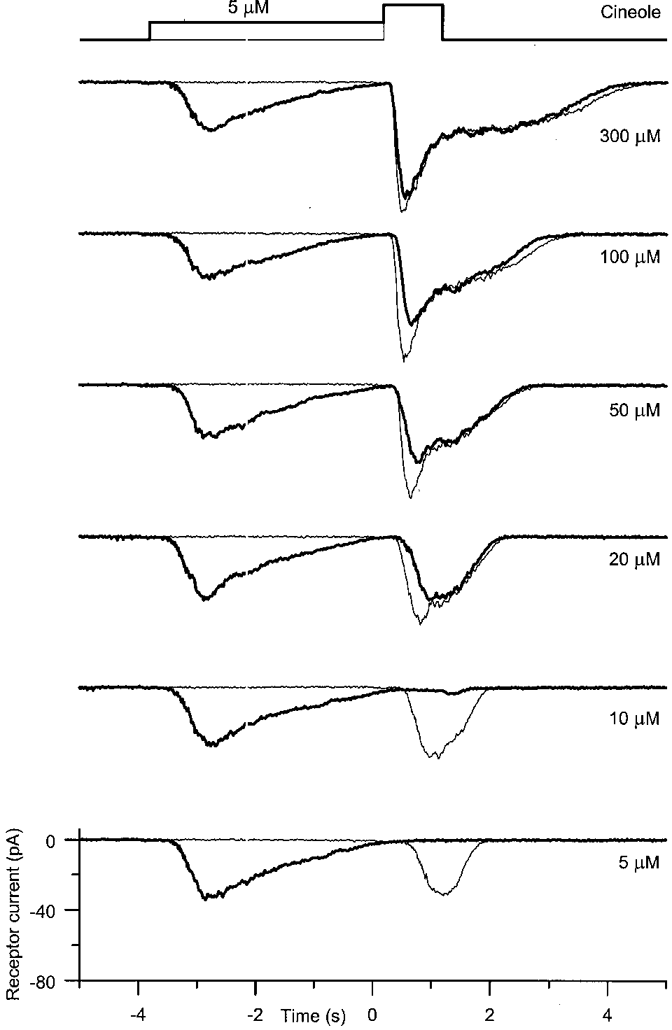
\includegraphics[width=0.5\linewidth]{figs/Reisert1999/fig_txn_compare_adaptation_R99_F4} }

}

\caption{Transduction figures from (Reisert 1999); (a) Receptor current responses of an olfactory receptor cell; (b) The effect of adaptation on the odour-induced receptor current}\label{fig:r99f24}
\end{figure}

\clearpage

\hypertarget{spikes-in-orn}{%
\subsection*{Spikes in ORN}\label{spikes-in-orn}}
\addcontentsline{toc}{subsection}{Spikes in ORN}

\begin{figure}

{\centering \subfloat[Reisert 1999 - Fig-1\label{fig:r99f13-1}]{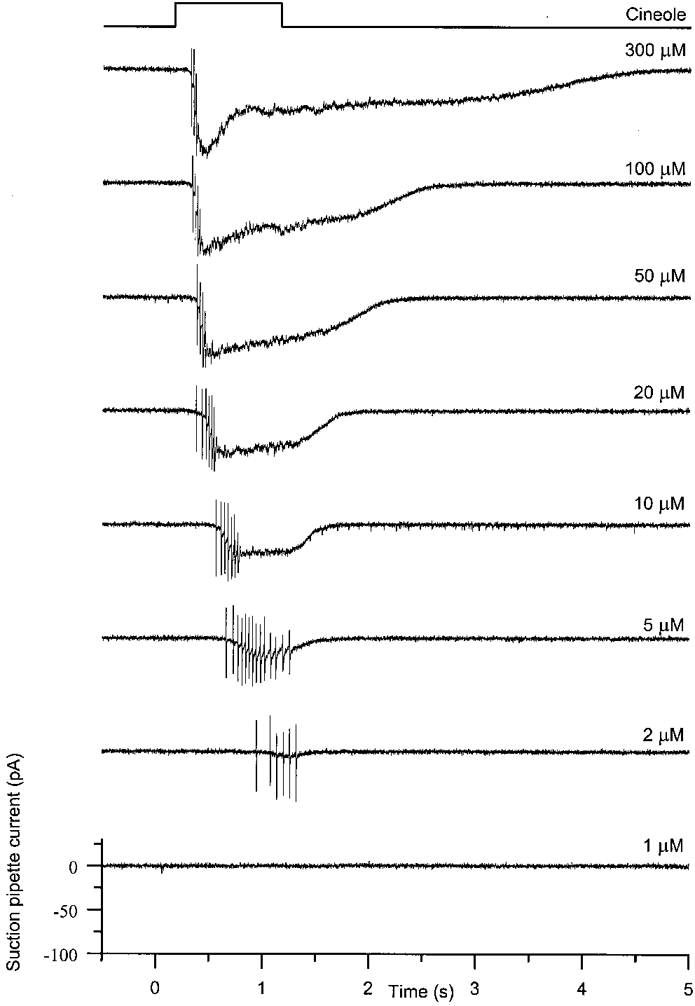
\includegraphics[width=0.5\linewidth]{figs/Reisert1999/fig_spk_compare_conc_R99_F1} }\subfloat[Reisert 1999 - 3\label{fig:r99f13-2}]{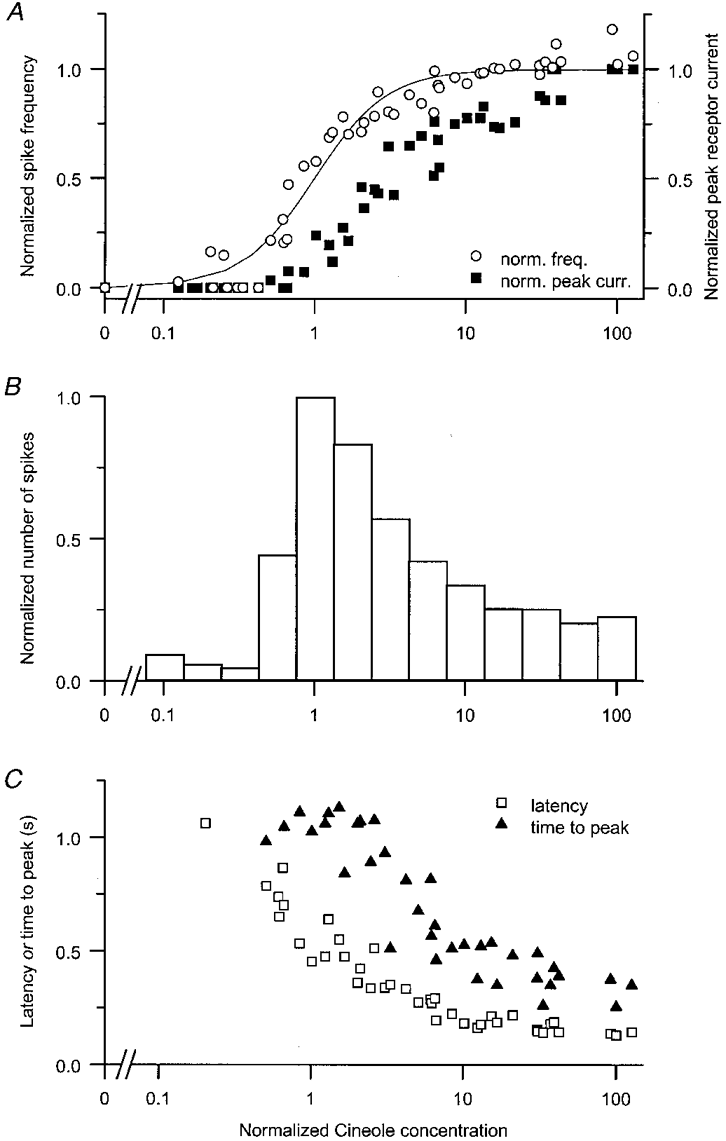
\includegraphics[width=0.5\linewidth]{figs/Reisert1999/fig_spk_compare_conc_quant_R99_F3} }

}

\caption{Spike-response profiling figures (Reisert 1999); (a) Responses of an olfactory receptor cell to odour stimuli of increasing concentration recorded with the suction pipette technique; (b) Collected dose-response data from six cells}\label{fig:r99f13}
\end{figure}

\begin{figure}

{\centering 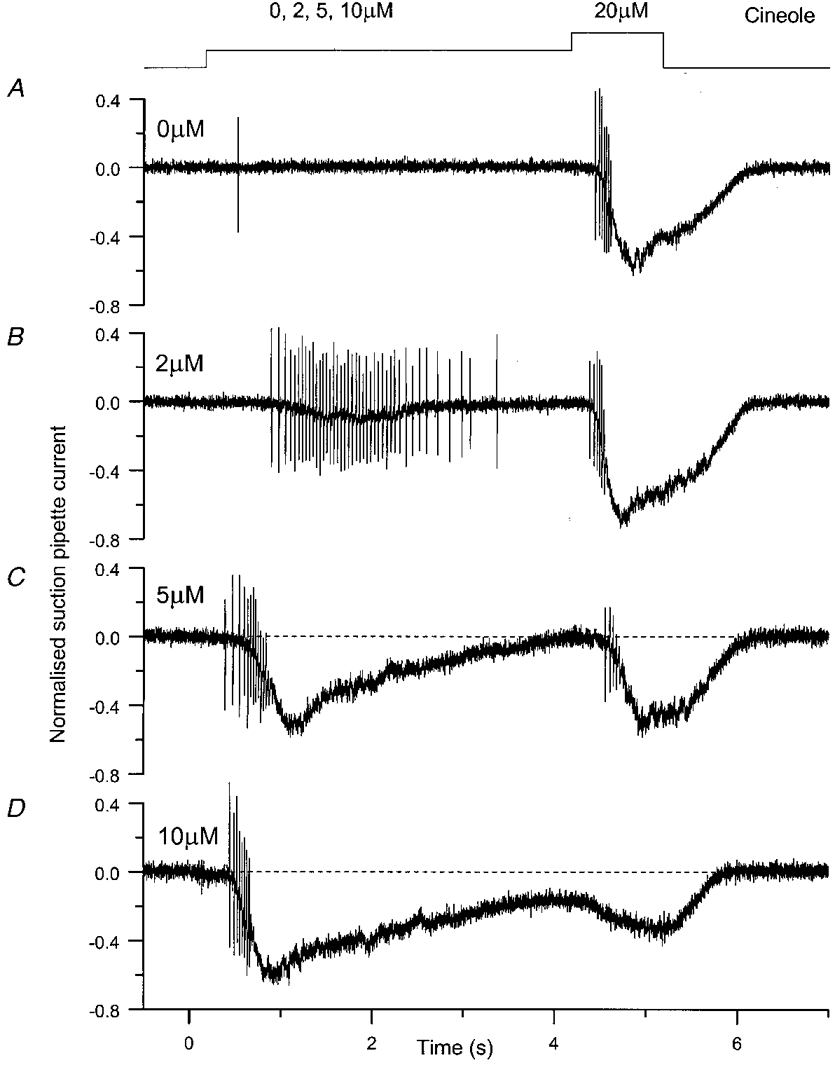
\includegraphics[width=0.8\linewidth]{figs/Reisert1999/fig_spk_compare_adaptation_R99_F5} 

}

\caption{The effect of adaptation on the odour-induced spike firing response (Fig-5; Reisert 1999)}\label{fig:r99f5}
\end{figure}

\clearpage

\hypertarget{appendix-b-supplimentary-plots}{%
\section*{Appendix B : Supplimentary plots}\label{appendix-b-supplimentary-plots}}
\addcontentsline{toc}{section}{Appendix B : Supplimentary plots}

\hypertarget{differences-in-adding-morris-lecar-dynamics}{%
\subsubsection*{Differences in adding Morris-Lecar dynamics}\label{differences-in-adding-morris-lecar-dynamics}}
\addcontentsline{toc}{subsubsection}{Differences in adding Morris-Lecar dynamics}

\begin{figure}

{\centering 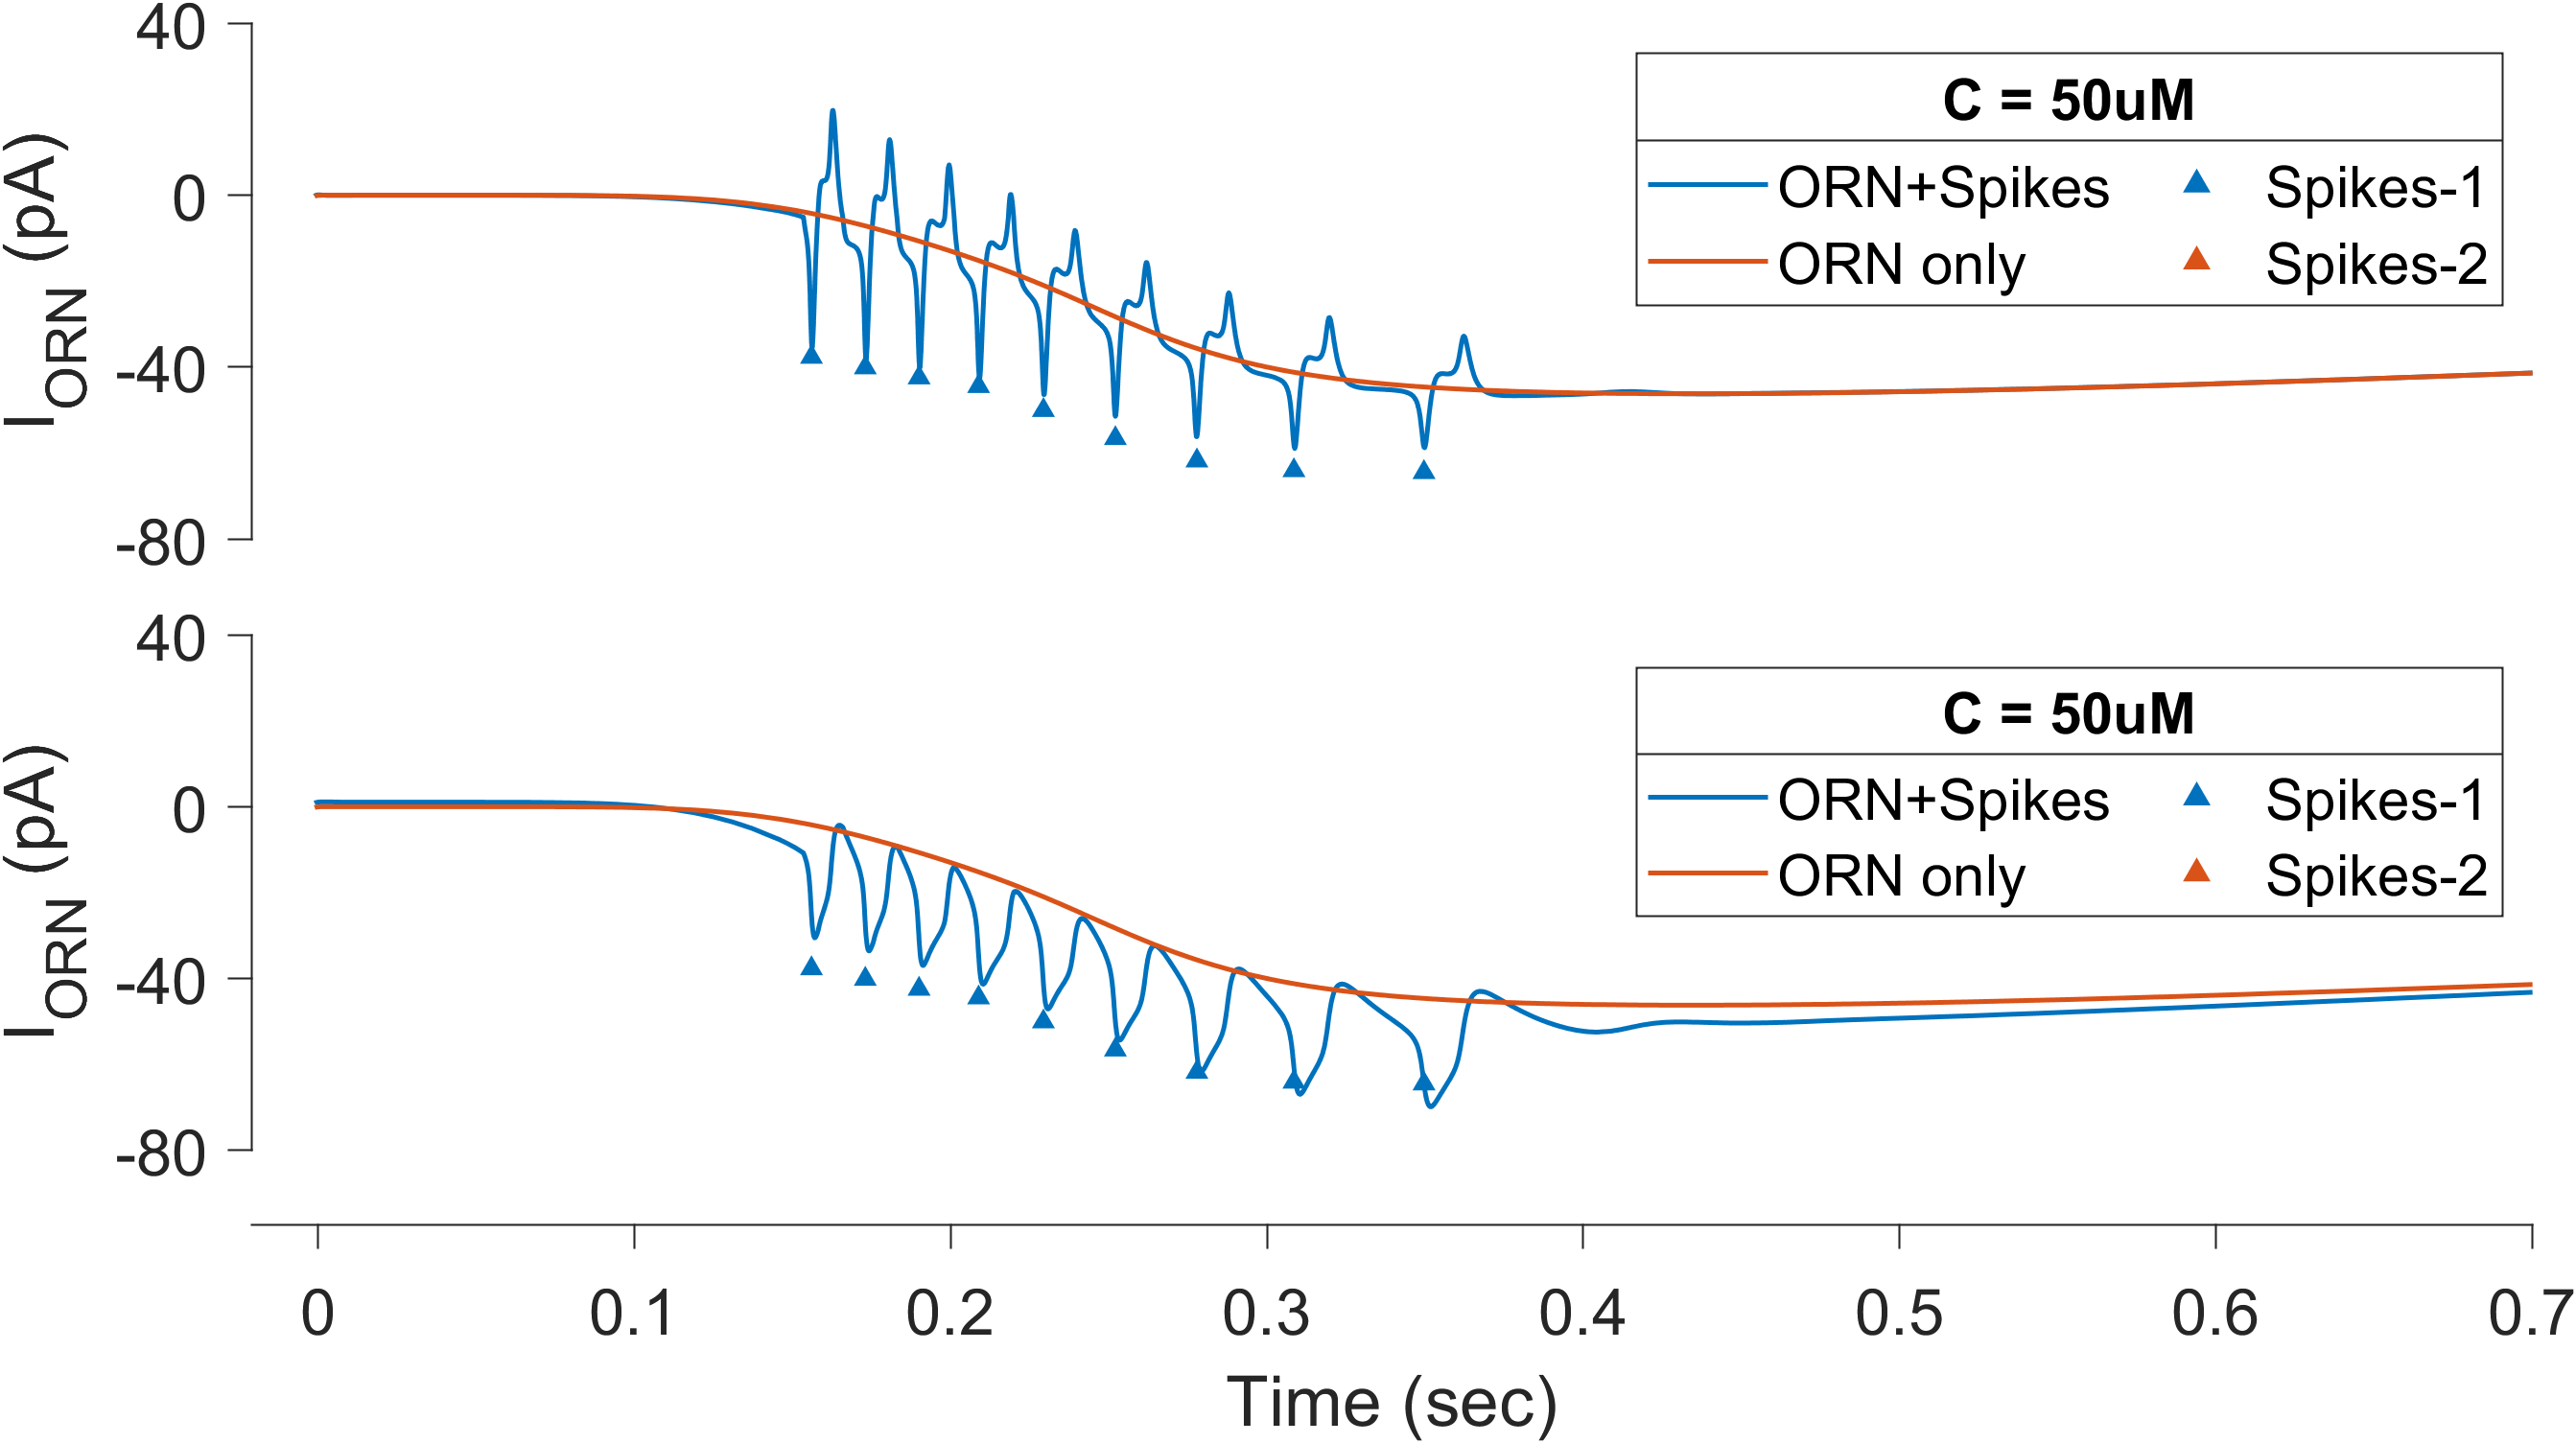
\includegraphics[width=0.8\linewidth]{figs/Appendix/supp_fig_ML_spikes_OVERLAP} 

}

\caption{Simulations with ML integrated into molecular process (top) and added ML-spikes separately post-simulation (bottom)}\label{fig:MLover}
\end{figure}

\hypertarget{effect-of-cafr}{%
\subsubsection*{Effect of CaFR}\label{effect-of-cafr}}
\addcontentsline{toc}{subsubsection}{Effect of CaFR}

\begin{figure}

{\centering 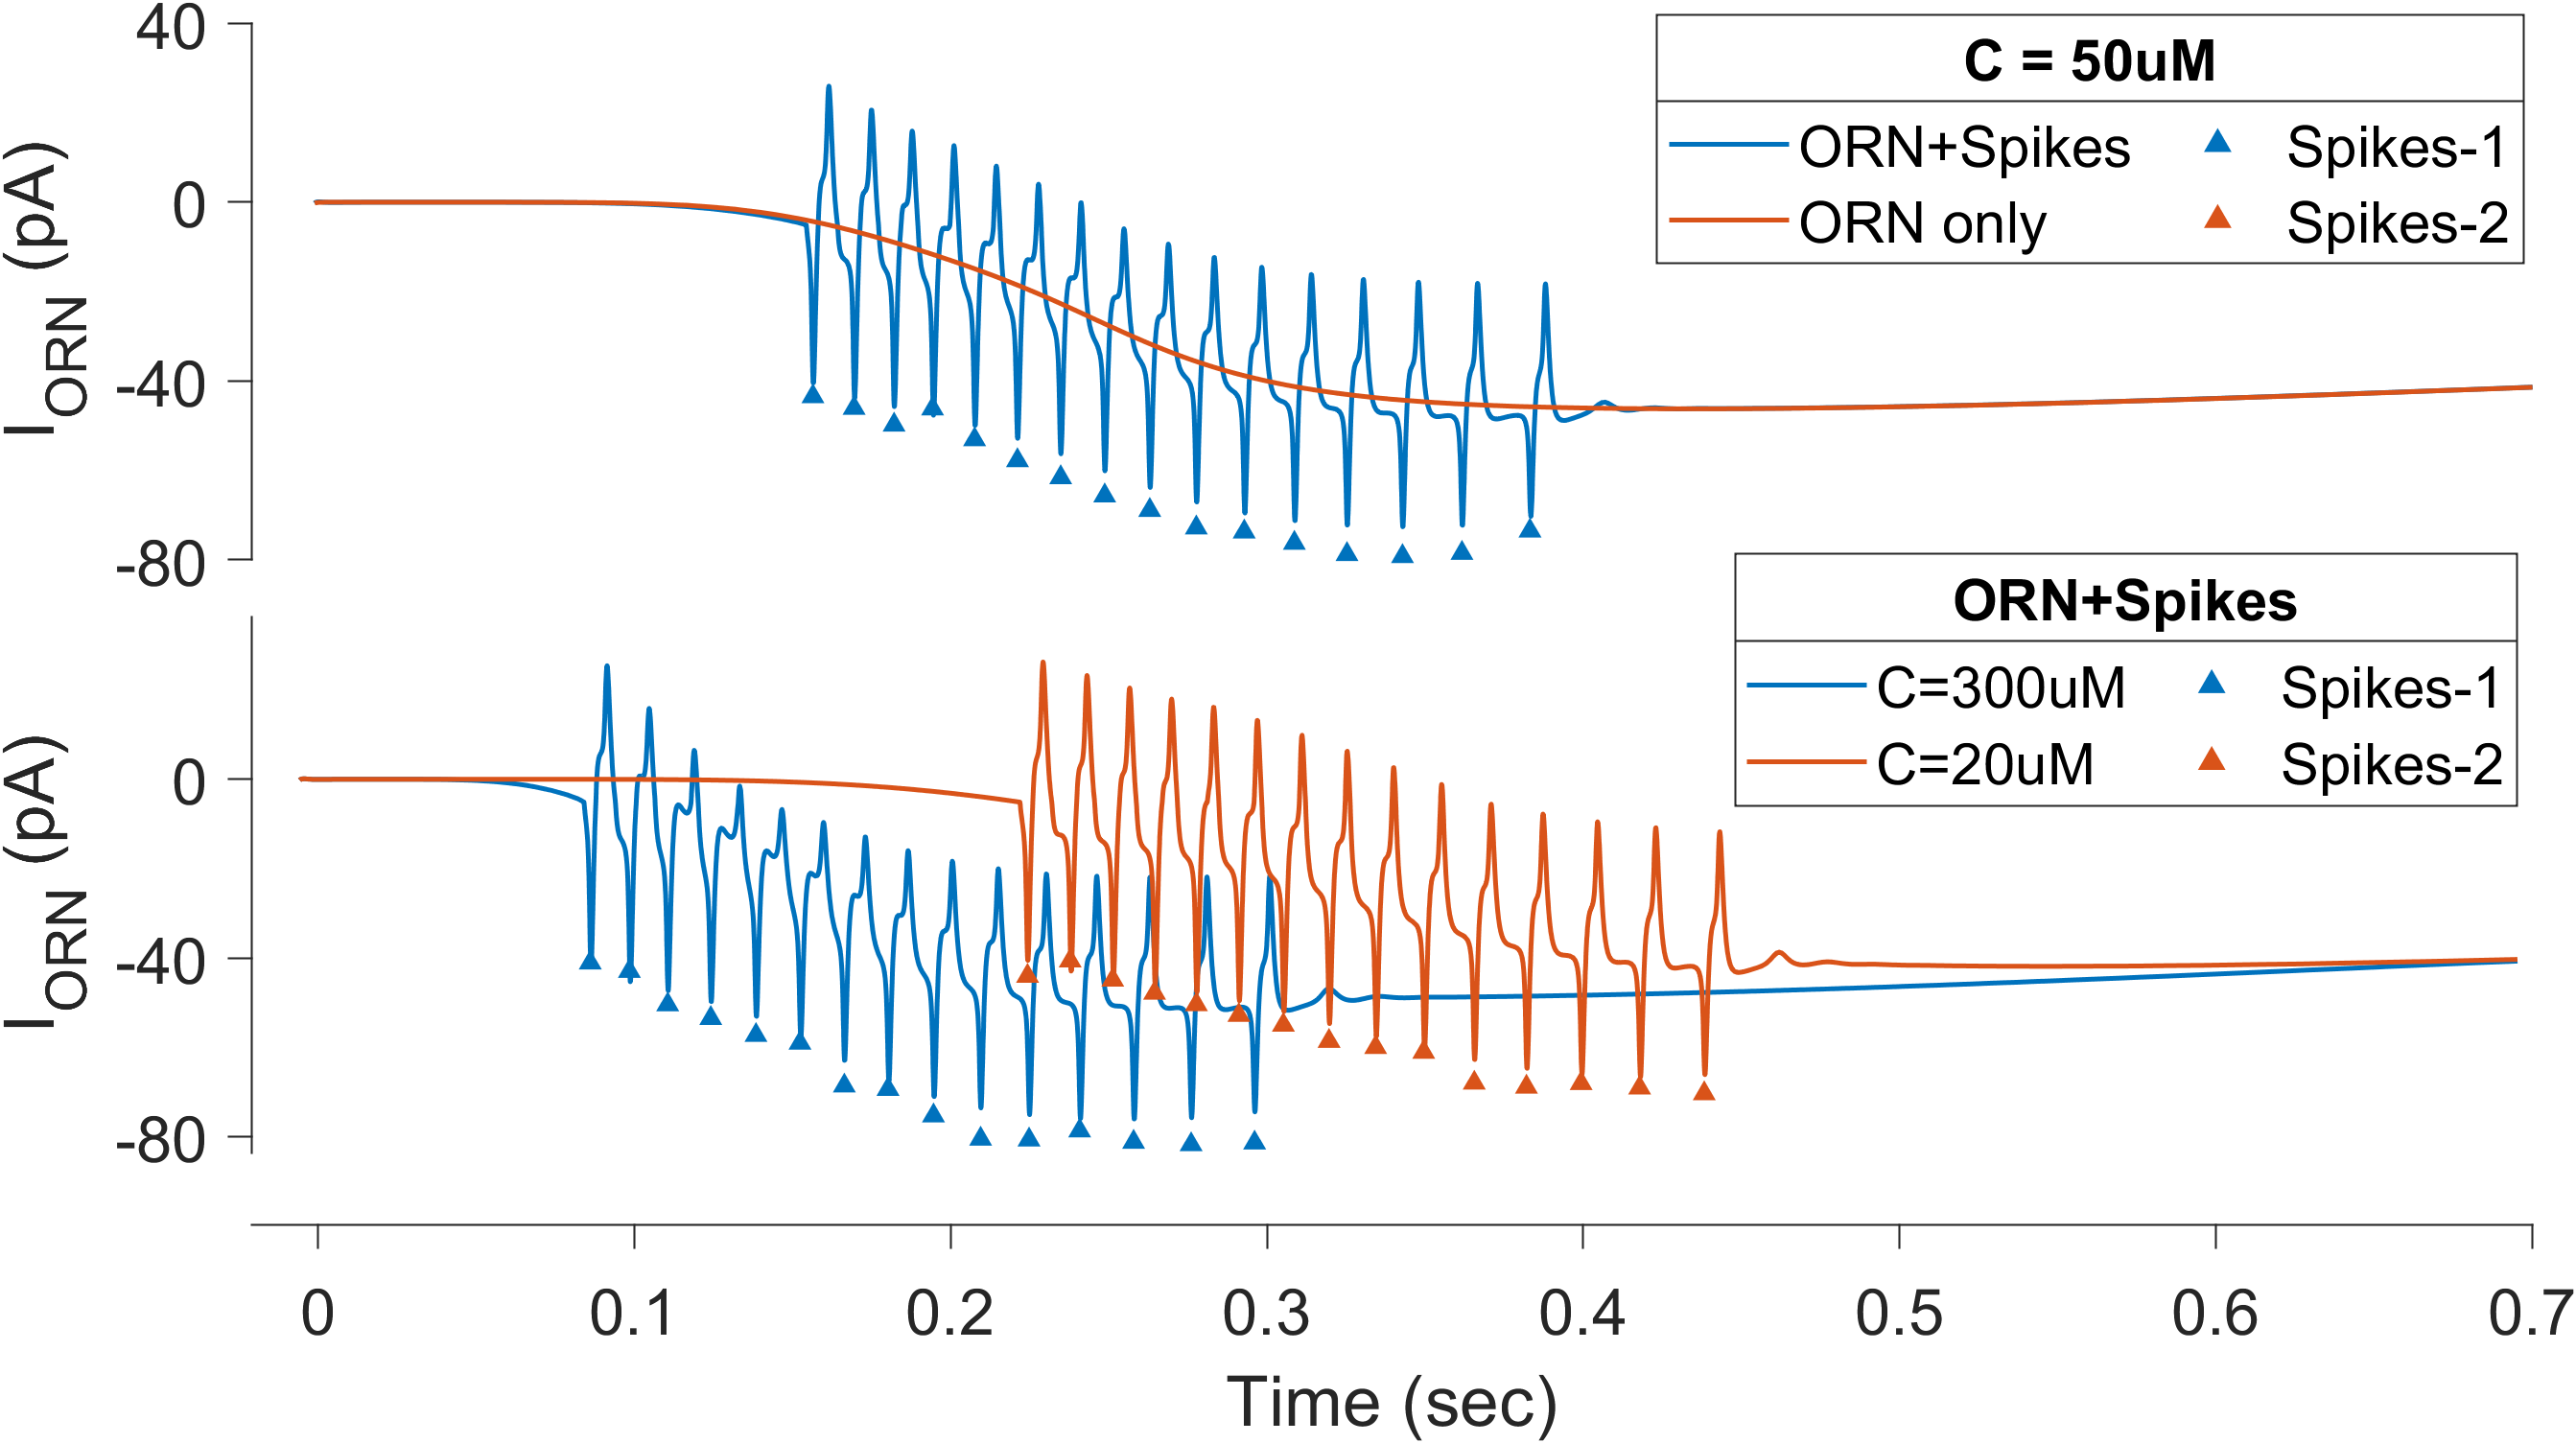
\includegraphics[width=0.8\linewidth]{figs/Appendix/supp_fig_ML_ID_w_CaFR_1} 

}

\caption{Simulations with keeping CaFR=1 for the entire duration}\label{fig:aCaFR1}
\end{figure}

\clearpage

\hypertarget{appendix-c-sniffing-simulation-raw-data-plots}{%
\section*{Appendix C : Sniffing-simulation raw-data plots}\label{appendix-c-sniffing-simulation-raw-data-plots}}
\addcontentsline{toc}{section}{Appendix C : Sniffing-simulation raw-data plots}

\begin{figure}

{\centering 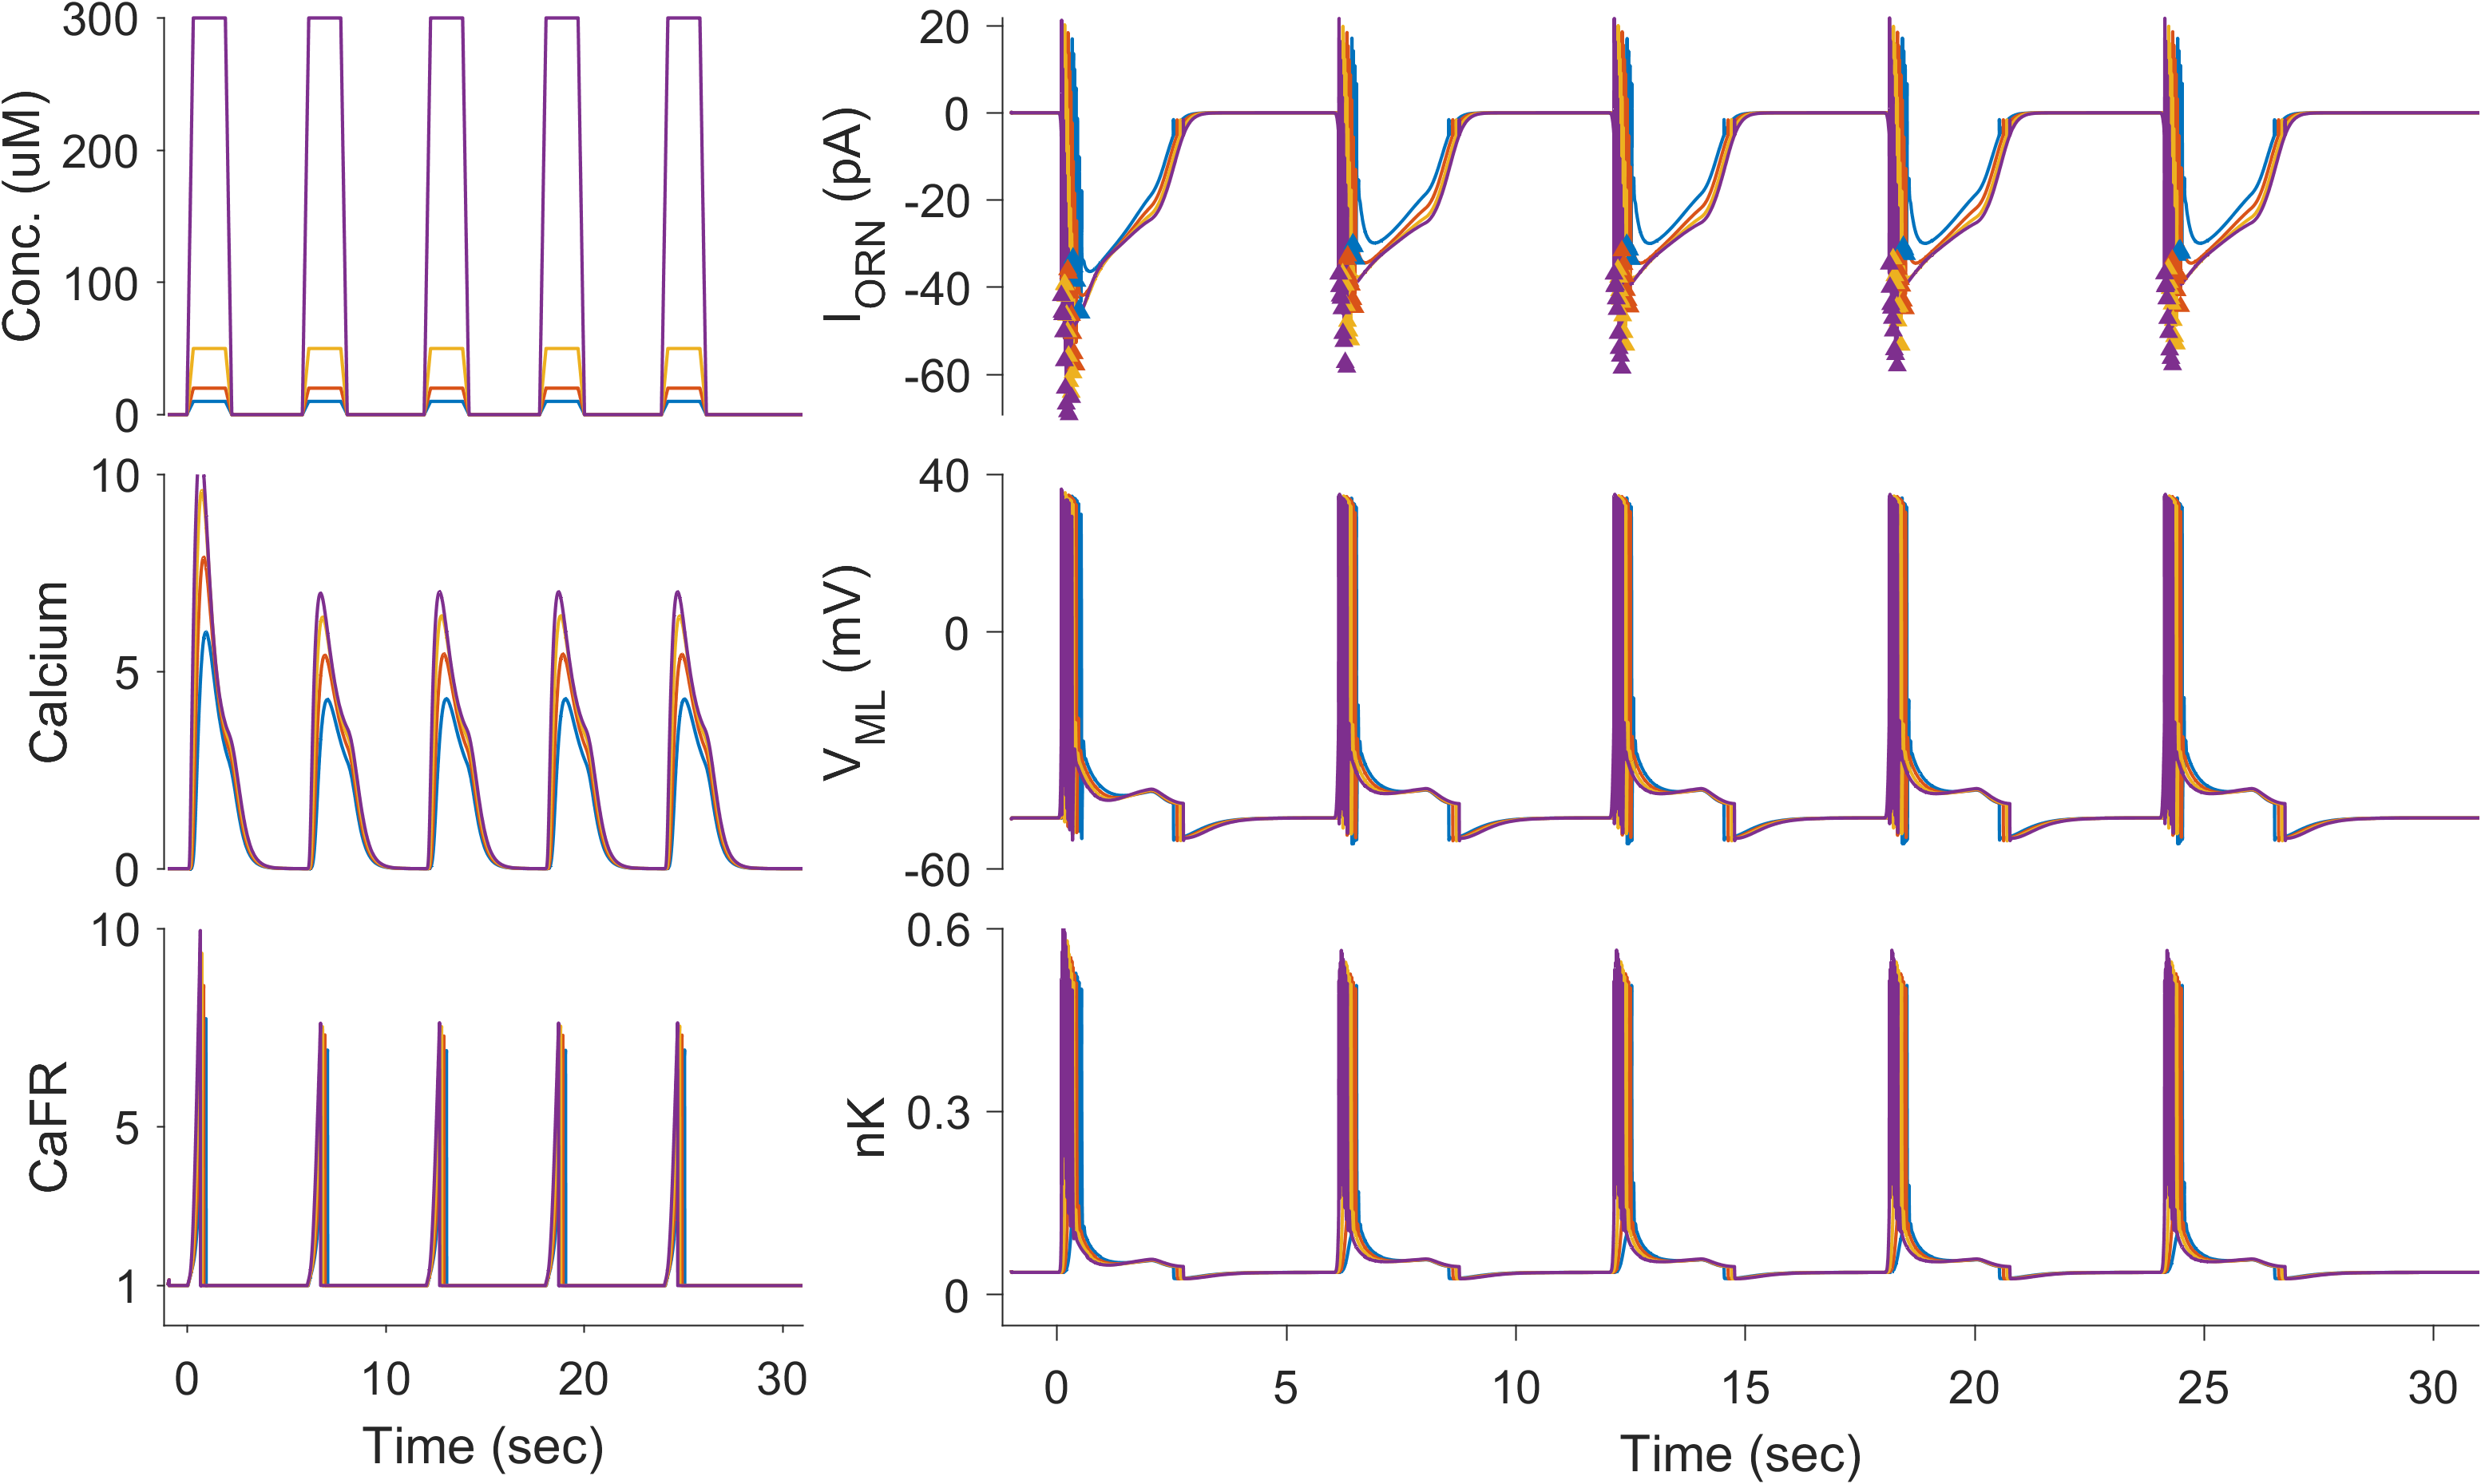
\includegraphics[width=0.95\linewidth]{figs/sniff/fig_spk_sniffing_10bpm} 

}

\caption{Sniffing at 10 breaths/min over-all}\label{fig:f10bpm}
\end{figure}

\begin{figure}

{\centering 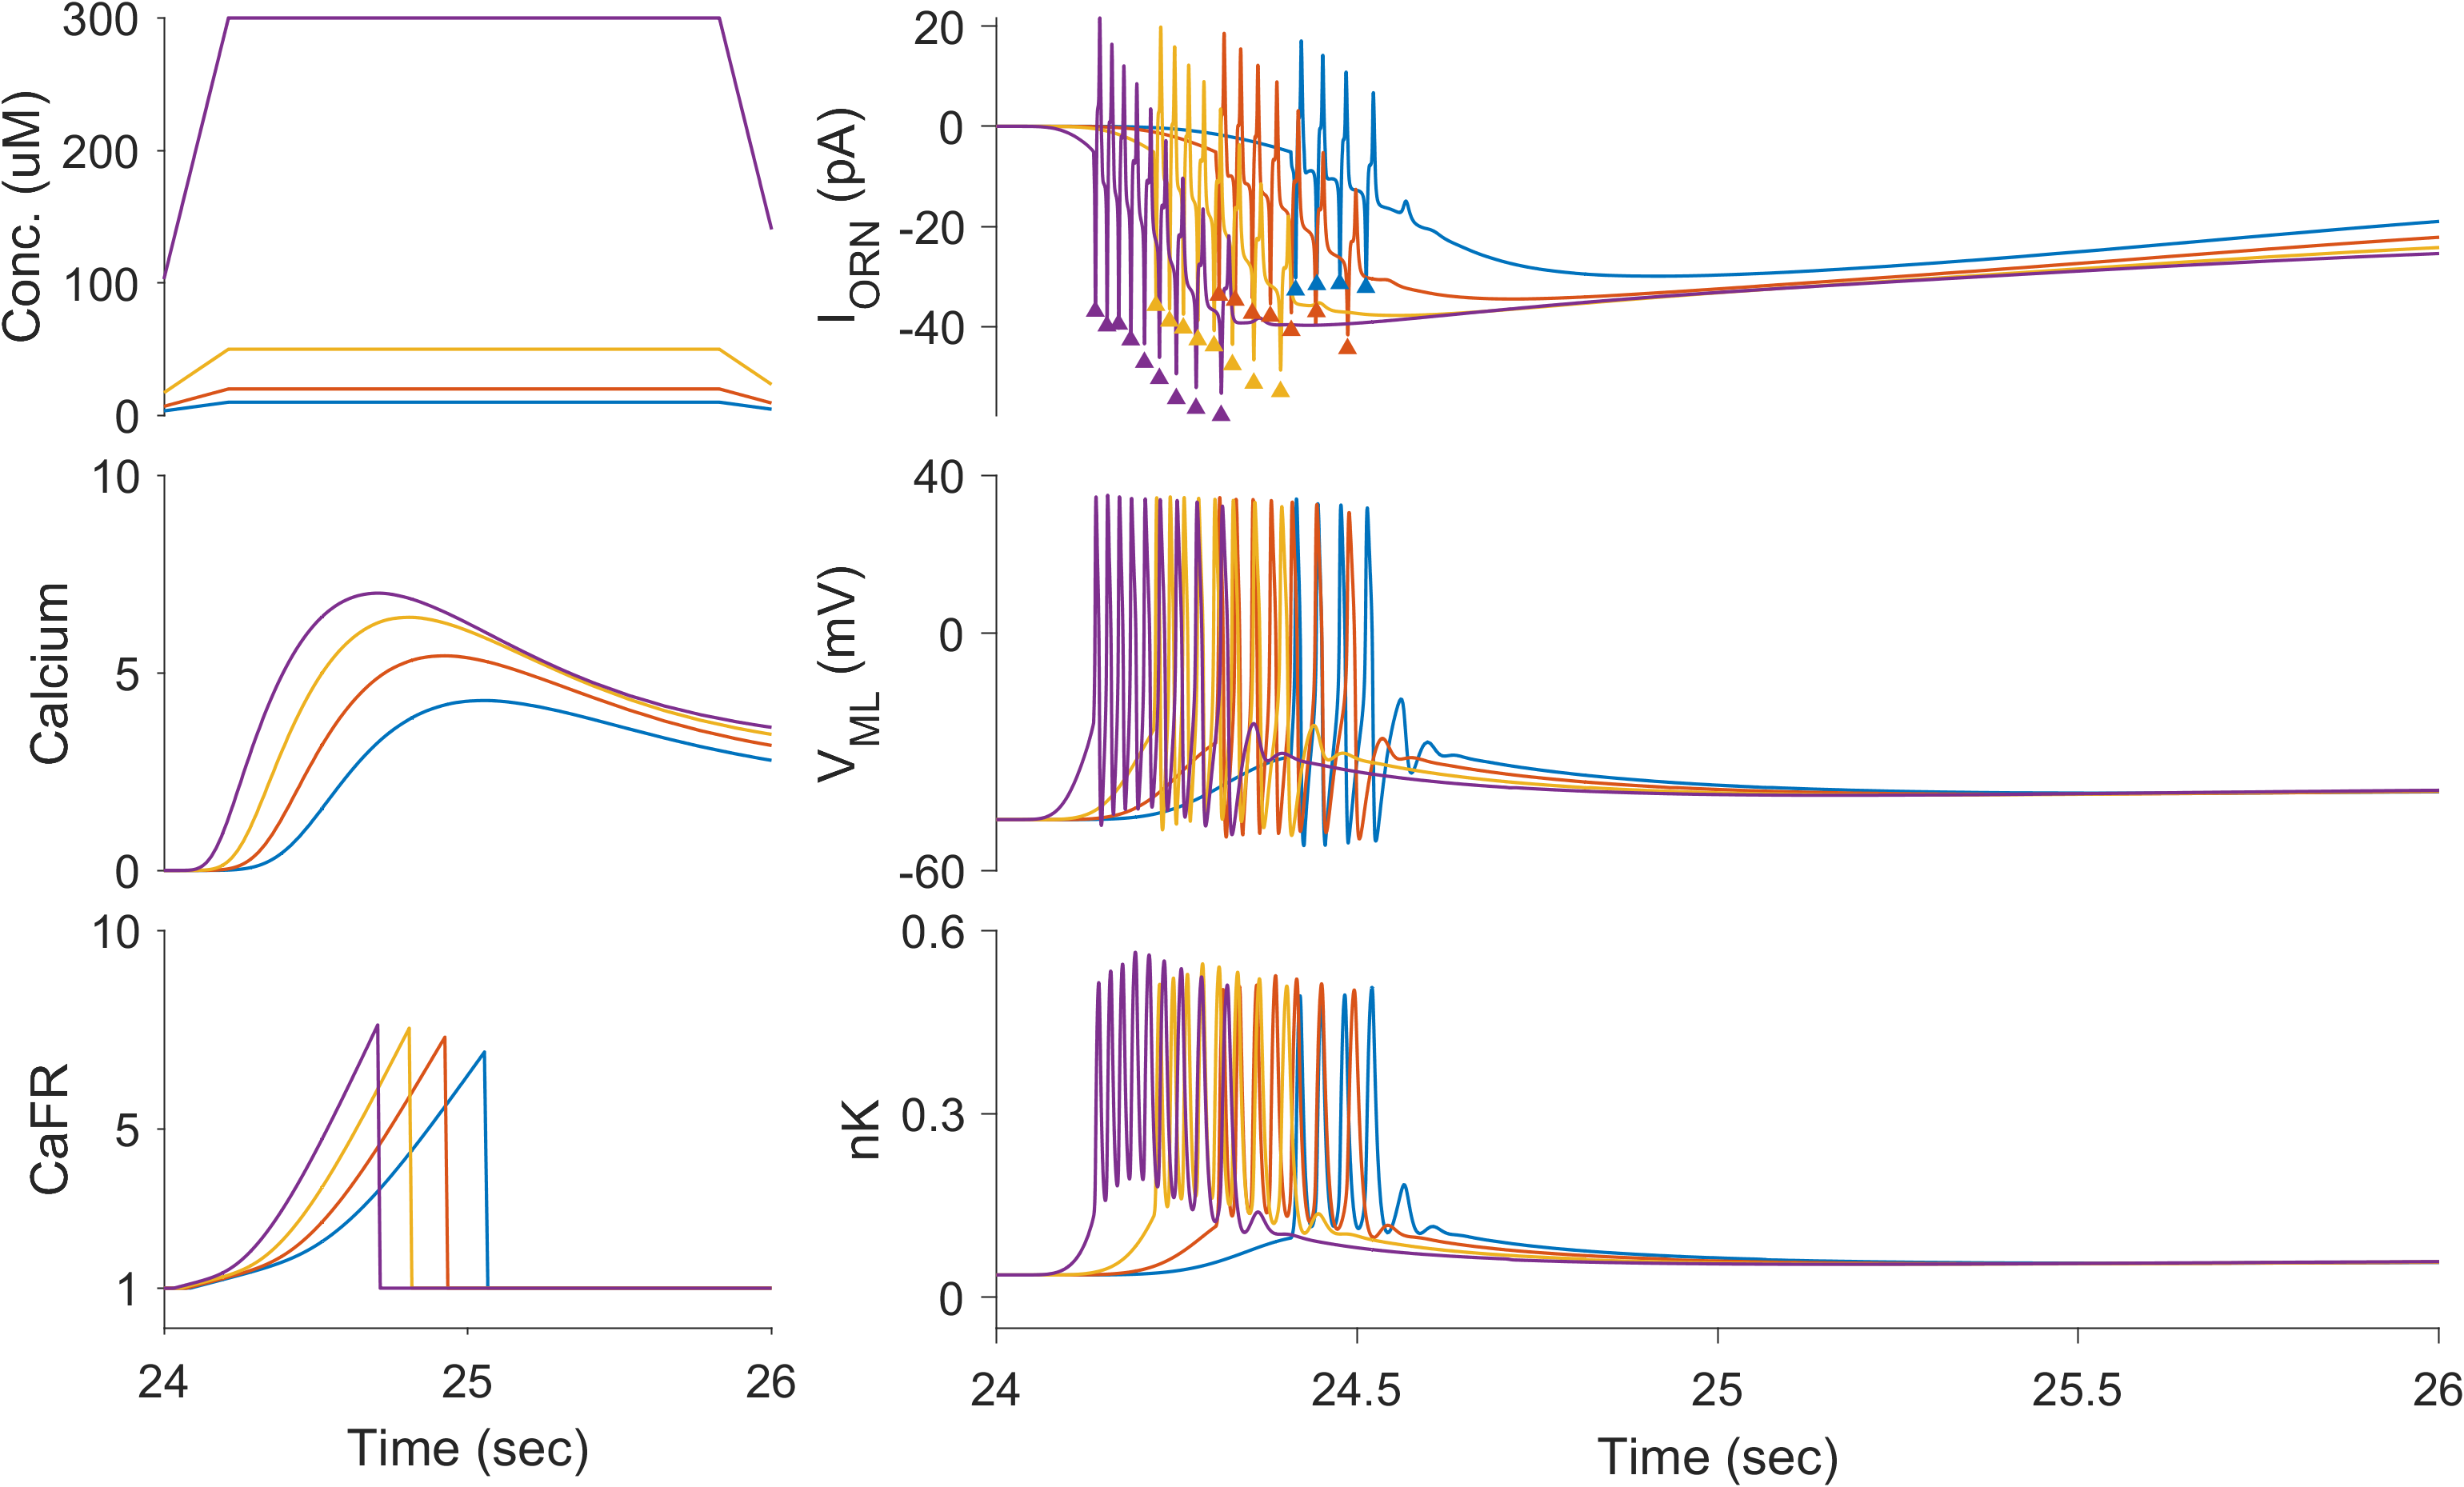
\includegraphics[width=0.95\linewidth]{figs/sniff/fig_spk_sniffing_10bpm_last} 

}

\caption{Sniffing at 10 breaths/min : steady-state response zoom-in}\label{fig:f10bpmSS}
\end{figure}

\begin{figure}

{\centering 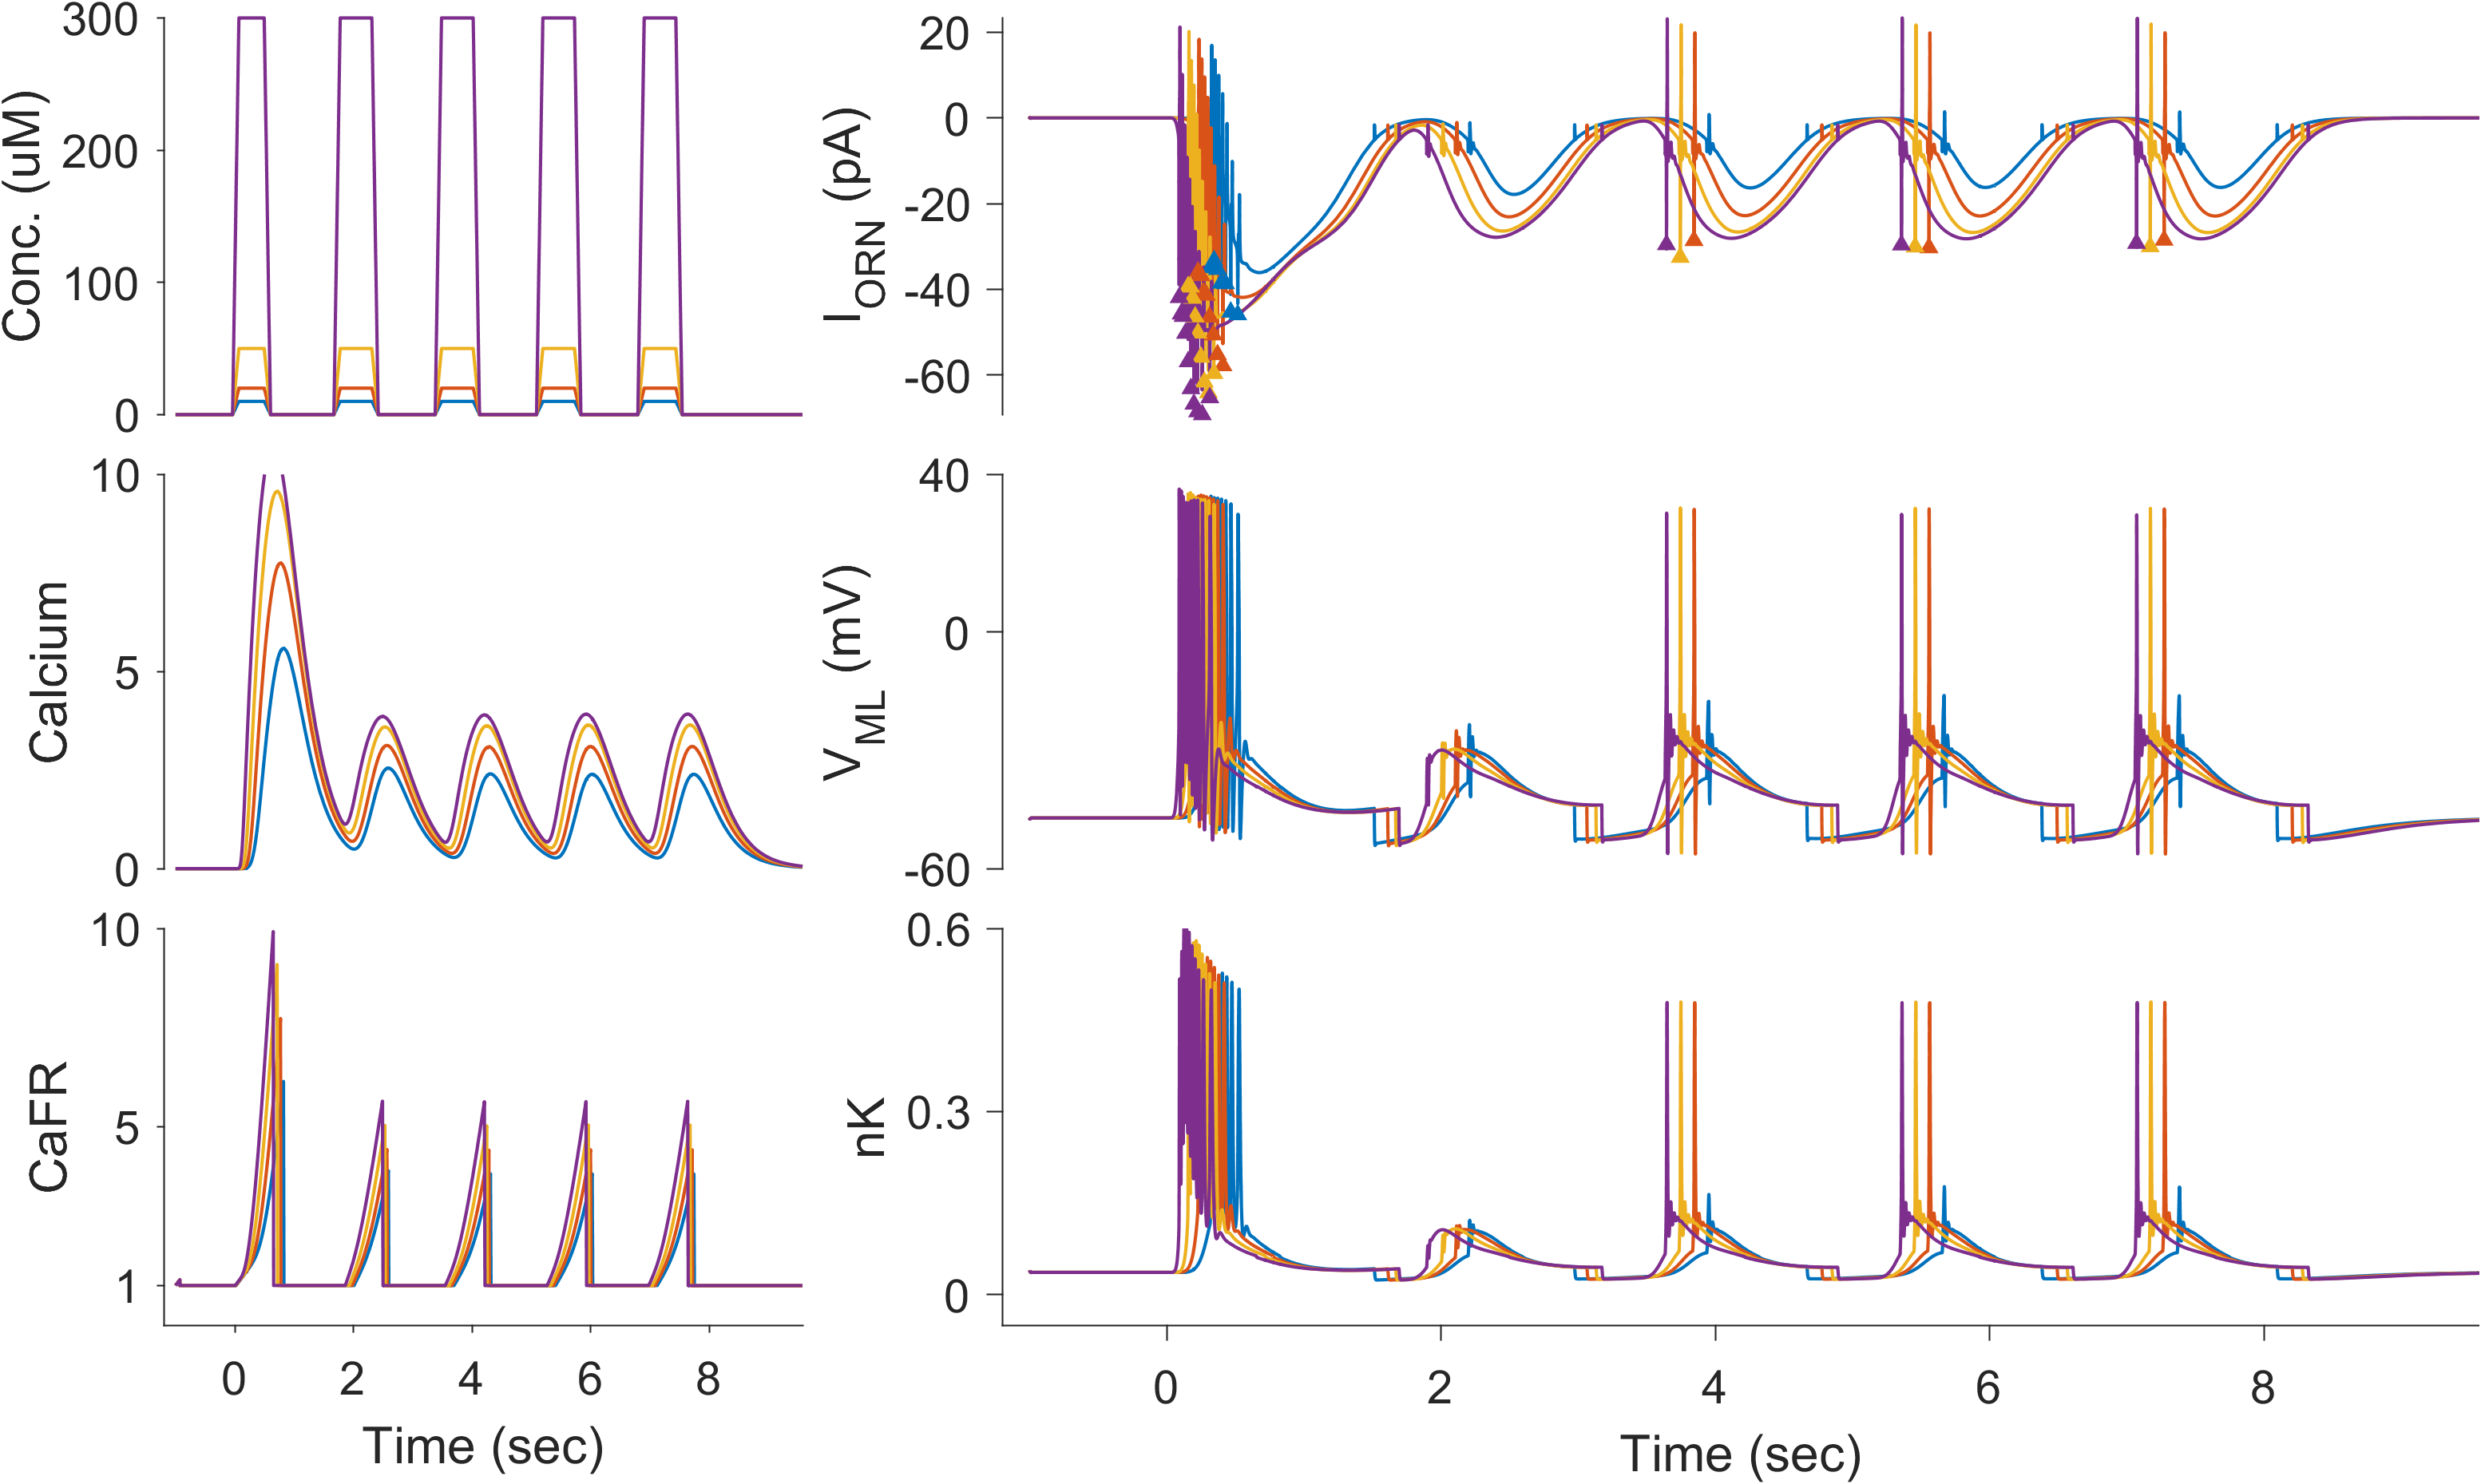
\includegraphics[width=0.95\linewidth]{figs/sniff/fig_spk_sniffing_35bpm} 

}

\caption{Sniffing at 35 breaths/min over-all}\label{fig:f35bpm}
\end{figure}

\begin{figure}

{\centering 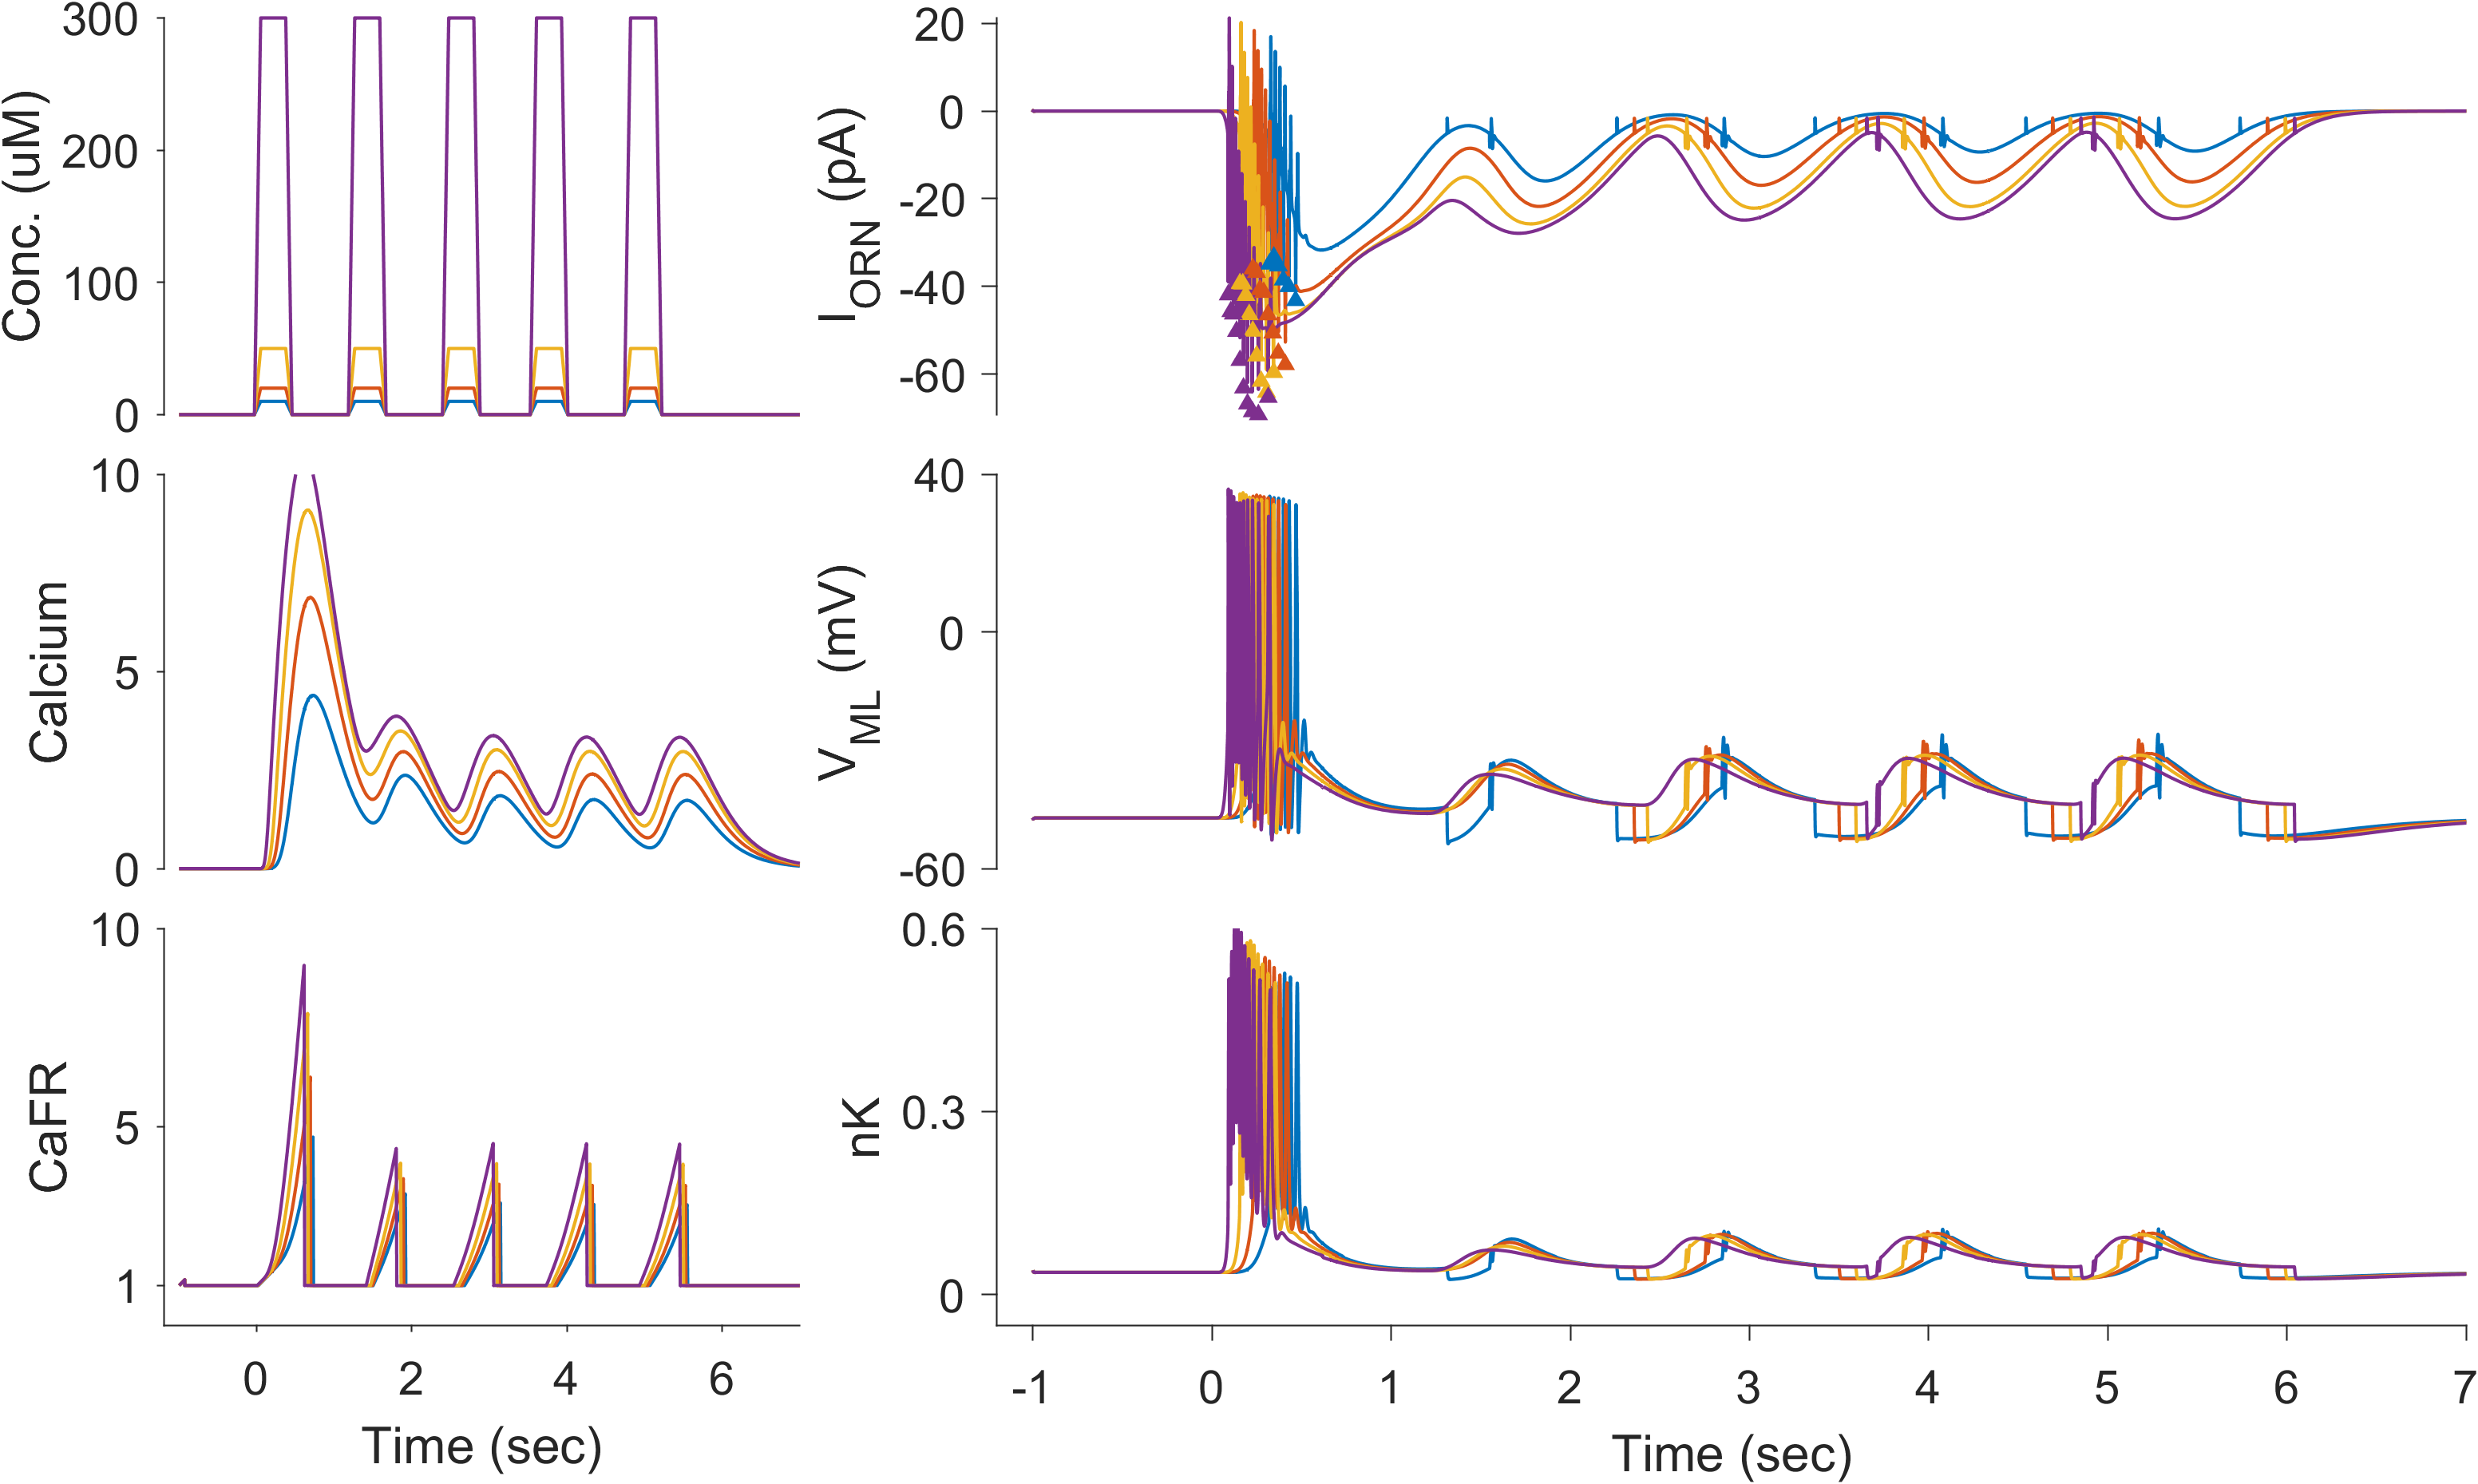
\includegraphics[width=0.95\linewidth]{figs/sniff/fig_spk_sniffing_50bpm} 

}

\caption{Sniffing at 50 breaths/min over-all}\label{fig:f50bpm}
\end{figure}

\clearpage

\hypertarget{appendix-d-codes}{%
\section*{Appendix D : Codes}\label{appendix-d-codes}}
\addcontentsline{toc}{section}{Appendix D : Codes}

\hypertarget{parameters}{%
\subsection*{Parameters}\label{parameters}}
\addcontentsline{toc}{subsection}{Parameters}

\begin{Shaded}
\begin{Highlighting}[]
\CommentTok{\%\% ORN System co{-}eff}
\NormalTok{P }\OperatorTok{=} \FunctionTok{struct}\NormalTok{(}\StringTok{\textquotesingle{}Sigma\textquotesingle{}}\OperatorTok{,}\FloatTok{0.0569}\OperatorTok{,} \StringTok{\textquotesingle{}cap\textquotesingle{}}\OperatorTok{,}\FloatTok{0.0039}\OperatorTok{,} \StringTok{\textquotesingle{}cc1lin\textquotesingle{}}\OperatorTok{,}\FloatTok{0.7750}\OperatorTok{,...}
        \StringTok{\textquotesingle{}cc2\textquotesingle{}}\OperatorTok{,}\FloatTok{26.3950}\OperatorTok{,}\StringTok{\textquotesingle{}ck1lin\textquotesingle{}}\OperatorTok{,}\FloatTok{8.5342}\OperatorTok{,}\StringTok{\textquotesingle{}ck2\textquotesingle{}}\OperatorTok{,}\FloatTok{0.3069}\OperatorTok{,}\StringTok{\textquotesingle{}clmax\textquotesingle{}}\OperatorTok{,}\FloatTok{0.9397}\OperatorTok{,...}
        \StringTok{\textquotesingle{}cnmax\textquotesingle{}}\OperatorTok{,}\FloatTok{0.9663}\OperatorTok{,}\StringTok{\textquotesingle{}cx1lin\textquotesingle{}}\OperatorTok{,}\FloatTok{1.2307}\OperatorTok{,}\StringTok{\textquotesingle{}cx2\textquotesingle{}}\OperatorTok{,}\FloatTok{10.9297}\OperatorTok{,}\StringTok{\textquotesingle{}ef\textquotesingle{}}\OperatorTok{,}\FloatTok{2.7583}\OperatorTok{,...}
        \StringTok{\textquotesingle{}gl\textquotesingle{}}\OperatorTok{,}\FloatTok{4.9195}\OperatorTok{,}\StringTok{\textquotesingle{}hmc1\textquotesingle{}}\OperatorTok{,}\FloatTok{1.4829}\OperatorTok{,}\StringTok{\textquotesingle{}hmc2\textquotesingle{}}\OperatorTok{,}\FloatTok{2.7678}\OperatorTok{,}\StringTok{\textquotesingle{}inf\textquotesingle{}}\OperatorTok{,}\FloatTok{1.7619}\OperatorTok{,}\StringTok{\textquotesingle{}inhmax\textquotesingle{}}\OperatorTok{,}\FloatTok{3.5697}\OperatorTok{,...}
        \StringTok{\textquotesingle{}k1\textquotesingle{}}\OperatorTok{,}\FloatTok{0.1143}\OperatorTok{,}\StringTok{\textquotesingle{}k2lin\textquotesingle{}}\OperatorTok{,}\FloatTok{12.9344}\OperatorTok{,}\StringTok{\textquotesingle{}kI\textquotesingle{}}\OperatorTok{,}\FloatTok{10.0453}\OperatorTok{,}\StringTok{\textquotesingle{}kinh\textquotesingle{}}\OperatorTok{,}\FloatTok{1.0018}\OperatorTok{,}\StringTok{\textquotesingle{}kinhcng\textquotesingle{}}\OperatorTok{,}\FloatTok{0.5181}\OperatorTok{,...}
        \StringTok{\textquotesingle{}n1\textquotesingle{}}\OperatorTok{,}\FloatTok{3.1844}\OperatorTok{,}\StringTok{\textquotesingle{}n2\textquotesingle{}}\OperatorTok{,}\FloatTok{3.1128}\OperatorTok{,}\StringTok{\textquotesingle{}nI\textquotesingle{}}\OperatorTok{,}\FloatTok{1.9848}\OperatorTok{,}\StringTok{\textquotesingle{}ninh\textquotesingle{}}\OperatorTok{,}\FloatTok{1.3081}\OperatorTok{,}\StringTok{\textquotesingle{}ninhcng\textquotesingle{}}\OperatorTok{,}\FloatTok{1.4511}\OperatorTok{,...}
        \StringTok{\textquotesingle{}pd\textquotesingle{}}\OperatorTok{,}\FloatTok{7.5749}\OperatorTok{,}\StringTok{\textquotesingle{}r1\textquotesingle{}}\OperatorTok{,}\FloatTok{3.1663}\OperatorTok{,}\StringTok{\textquotesingle{}r2\textquotesingle{}}\OperatorTok{,}\FloatTok{6.5597}\OperatorTok{,}\StringTok{\textquotesingle{}smax\textquotesingle{}}\OperatorTok{,}\FloatTok{45.5118}\OperatorTok{,}\StringTok{\textquotesingle{}vcl\textquotesingle{}}\OperatorTok{,{-}}\FloatTok{7.7902}\OperatorTok{,...}
        \StringTok{\textquotesingle{}vcng\textquotesingle{}}\OperatorTok{,}\FloatTok{0.0106}\OperatorTok{,}\StringTok{\textquotesingle{}vl\textquotesingle{}}\OperatorTok{,{-}}\FloatTok{44.0413}\NormalTok{)}\OperatorTok{;}

\CommentTok{\%\% ML Spike sytem co{-}eff}
\NormalTok{S }\OperatorTok{=} \FunctionTok{struct}\OperatorTok{;}
\NormalTok{S.SpikeEN }\OperatorTok{=} \FloatTok{1}\OperatorTok{;} \CommentTok{\% EN=1, DL=0}
\CommentTok{\% Spike properties}
\NormalTok{S.spkThr }\OperatorTok{=} \OperatorTok{{-}}\FloatTok{43}\OperatorTok{;} \CommentTok{\% (ORN\_rest={-}44) mV}
\NormalTok{S.maxFR }\OperatorTok{=} \FloatTok{50}\OperatorTok{;} \CommentTok{\% Max firing rate Hz}
\NormalTok{S.revCp }\OperatorTok{=} \FloatTok{0.3}\OperatorTok{;} \CommentTok{\% Reverse coupling from spkV to mem.Voltage}

\CommentTok{\% Ca2+ dependent firing rate modulation }
\NormalTok{S.mCaFR }\OperatorTok{=} \FloatTok{1}\OperatorTok{;}\NormalTok{ S.pCaFR }\OperatorTok{=} \FloatTok{2}\OperatorTok{;}\NormalTok{ S.nCaFR }\OperatorTok{=} \FloatTok{100}\OperatorTok{;} \CommentTok{\%(min,pos,neg)}
\NormalTok{S.gIca }\OperatorTok{=} \FloatTok{10}\OperatorTok{;} \CommentTok{\% Ca@+ current gain}
\NormalTok{S.gIion }\OperatorTok{=} \FloatTok{22}\OperatorTok{;} \CommentTok{\% other ion channels activation}

\CommentTok{\% ML Mem. volt. parameters, adapted from (Anderson et. al., 2015)}
\NormalTok{S.vCa }\OperatorTok{=} \FloatTok{120}\OperatorTok{;}                \CommentTok{\% Rev.Pot for Calcium channels}
\NormalTok{S.gCa }\OperatorTok{=} \FloatTok{4.4}\OperatorTok{;}                \CommentTok{\% Calcium conductance}
\NormalTok{S.vK  }\OperatorTok{=} \OperatorTok{{-}}\FloatTok{84}\OperatorTok{;}                \CommentTok{\% Rev.Pot for Potassium channels}
\NormalTok{S.gK  }\OperatorTok{=}   \FloatTok{8}\OperatorTok{;}                \CommentTok{\% Potassium conductance}
\NormalTok{S.vL  }\OperatorTok{=} \OperatorTok{{-}}\FloatTok{44}\OperatorTok{;} \CommentTok{\% {-}60          \% Rev.Pot for leak channels}
\NormalTok{S.gL  }\OperatorTok{=}   \FloatTok{2}\OperatorTok{;}                \CommentTok{\% Leak channels conductance}
\NormalTok{S.Cm  }\OperatorTok{=}  \FloatTok{20}\OperatorTok{;}                \CommentTok{\% Membrane Conductance}
\CommentTok{\% Ca2+ ion channel parameters}
\NormalTok{S.va }\OperatorTok{=} \OperatorTok{{-}}\FloatTok{1.2}\OperatorTok{;}\NormalTok{ S.vb }\OperatorTok{=} \FloatTok{18}\OperatorTok{;}
\CommentTok{\% K+ ion channel parameters}
\NormalTok{S.vc }\OperatorTok{=} \FloatTok{2}\OperatorTok{;}\NormalTok{ S.vd }\OperatorTok{=} \FloatTok{30}\OperatorTok{;}\NormalTok{ S.phi\_n }\OperatorTok{=} \FloatTok{0.04}\OperatorTok{;}
\CommentTok{\% Current normalizing factor}
\NormalTok{S.NF }\OperatorTok{=} \FloatTok{70}\OperatorTok{;}
\end{Highlighting}
\end{Shaded}

\hypertarget{orn-simulation}{%
\subsection*{ORN Simulation}\label{orn-simulation}}
\addcontentsline{toc}{subsection}{ORN Simulation}

\begin{Shaded}
\begin{Highlighting}[]
\ControlFlowTok{function}\NormalTok{ DATA }\OperatorTok{=}\NormalTok{ simulate\_ORN(PULSE}\OperatorTok{,}\NormalTok{SpikeEN}\OperatorTok{,}\NormalTok{P}\OperatorTok{,}\NormalTok{S) }

\ControlFlowTok{if} \OperatorTok{\textasciitilde{}}\FunctionTok{exist}\NormalTok{(}\StringTok{\textquotesingle{}S\textquotesingle{}}\OperatorTok{,}\StringTok{\textquotesingle{}var\textquotesingle{}}\NormalTok{) }\OperatorTok{||} \OperatorTok{\textasciitilde{}}\FunctionTok{exist}\NormalTok{(}\StringTok{\textquotesingle{}P\textquotesingle{}}\OperatorTok{,}\StringTok{\textquotesingle{}var\textquotesingle{}}\NormalTok{)}
\NormalTok{    simulation\_parameters}\OperatorTok{;}
\ControlFlowTok{end}

\ControlFlowTok{if} \FunctionTok{exist}\NormalTok{(}\StringTok{\textquotesingle{}SpikeEN\textquotesingle{}}\OperatorTok{,}\StringTok{\textquotesingle{}var\textquotesingle{}}\NormalTok{)}
\NormalTok{    S.SpikeEN }\OperatorTok{=}\NormalTok{ SpikeEN}\OperatorTok{;}
\ControlFlowTok{else}
\NormalTok{    S.SpikeEN }\OperatorTok{=} \FloatTok{1}\OperatorTok{;}
\ControlFlowTok{end}

\CommentTok{\% Initialize}
\NormalTok{init\_bLR    }\OperatorTok{=} \FloatTok{1}\NormalTok{.e}\OperatorTok{{-}}\FloatTok{8}\OperatorTok{;} \CommentTok{\%1}
\NormalTok{init\_aG     }\OperatorTok{=} \FloatTok{1}\NormalTok{.e}\OperatorTok{{-}}\FloatTok{8}\OperatorTok{;} \CommentTok{\%2}
\NormalTok{init\_cAMP   }\OperatorTok{=} \FloatTok{1}\NormalTok{.e}\OperatorTok{{-}}\FloatTok{8}\OperatorTok{;} \CommentTok{\%3}
\NormalTok{init\_Ca     }\OperatorTok{=} \FloatTok{1}\NormalTok{.e}\OperatorTok{{-}}\FloatTok{8}\OperatorTok{;} \CommentTok{\%4}
\NormalTok{init\_CAMK   }\OperatorTok{=} \FloatTok{1}\NormalTok{.e}\OperatorTok{{-}}\FloatTok{8}\OperatorTok{;} \CommentTok{\%5}
\NormalTok{init\_CaCAM  }\OperatorTok{=} \FloatTok{1}\NormalTok{.e}\OperatorTok{{-}}\FloatTok{8}\OperatorTok{;} \CommentTok{\%6}
\NormalTok{init\_IX     }\OperatorTok{=} \FloatTok{1}\NormalTok{.e}\OperatorTok{{-}}\FloatTok{8}\OperatorTok{;} \CommentTok{\%7}
\NormalTok{init\_ornV   }\OperatorTok{=} \OperatorTok{{-}}\FloatTok{44}\OperatorTok{;}   \CommentTok{\%8}
\NormalTok{init\_spkV   }\OperatorTok{=} \OperatorTok{{-}}\FloatTok{47.14}\OperatorTok{;} \CommentTok{\%9 ML dV/dt}
\NormalTok{init\_nk     }\OperatorTok{=} \FloatTok{0.04}\OperatorTok{;}  \CommentTok{\%10 ML dN/dt }
\NormalTok{init\_CaFR   }\OperatorTok{=} \FloatTok{1}\OperatorTok{;}     \CommentTok{\%11 ML d(slope)/dt}

\NormalTok{yinit }\OperatorTok{=}\NormalTok{ \{init\_bLR}\OperatorTok{,}\NormalTok{ init\_aG}\OperatorTok{,}\NormalTok{ init\_cAMP}\OperatorTok{,}\NormalTok{ init\_Ca}\OperatorTok{,...}
\NormalTok{        init\_CaCAM}\OperatorTok{,}\NormalTok{init\_CAMK}\OperatorTok{,}\NormalTok{init\_IX}\OperatorTok{,}\NormalTok{init\_ornV}\OperatorTok{,...}
\NormalTok{        init\_spkV}\OperatorTok{,}\NormalTok{ init\_nk}\OperatorTok{,}\NormalTok{ init\_CaFR\}}\OperatorTok{;}
\NormalTok{FN }\OperatorTok{=}\NormalTok{ \{}\StringTok{\textquotesingle{}bLR\textquotesingle{}}\OperatorTok{,}\StringTok{\textquotesingle{}aG\textquotesingle{}}\OperatorTok{,}\StringTok{\textquotesingle{}cAMP\textquotesingle{}}\OperatorTok{,}\StringTok{\textquotesingle{}Ca\textquotesingle{}}\OperatorTok{,...}
    \StringTok{\textquotesingle{}CaCaM\textquotesingle{}}\OperatorTok{,}\StringTok{\textquotesingle{}aCaMK\textquotesingle{}}\OperatorTok{,}\StringTok{\textquotesingle{}IX\textquotesingle{}}\OperatorTok{,}\StringTok{\textquotesingle{}ornV\textquotesingle{}}\OperatorTok{,...}
    \StringTok{\textquotesingle{}spkV\textquotesingle{}}\OperatorTok{,}\StringTok{\textquotesingle{}nK\textquotesingle{}}\OperatorTok{,}\StringTok{\textquotesingle{}CaFR\textquotesingle{}}\NormalTok{\}}\OperatorTok{;}
\NormalTok{yinit }\OperatorTok{=} \FunctionTok{cell2struct}\NormalTok{(yinit}\OperatorTok{,}\NormalTok{FN}\OperatorTok{,}\FloatTok{2}\NormalTok{)}\OperatorTok{;}
\NormalTok{N }\OperatorTok{=} \FunctionTok{size}\NormalTok{(PULSE.ton}\OperatorTok{,}\FloatTok{1}\NormalTok{)}\OperatorTok{;}
\NormalTok{var\_names }\OperatorTok{=} \FunctionTok{fieldnames}\NormalTok{(yinit)}\OperatorTok{;}
\NormalTok{init\_vals }\OperatorTok{=} \FunctionTok{struct2cell}\NormalTok{(yinit)}\OperatorTok{;}
\NormalTok{init\_vals }\OperatorTok{=}\NormalTok{ [init\_vals\{}\OperatorTok{:}\NormalTok{\}]}\OperatorTok{;}
\NormalTok{init\_vals }\OperatorTok{=} \FunctionTok{repmat}\NormalTok{(init\_vals(}\OperatorTok{:}\NormalTok{)}\OperatorTok{\textquotesingle{},}\NormalTok{N}\OperatorTok{,}\FloatTok{1}\NormalTok{)}\OperatorTok{;}
\NormalTok{init\_vals }\OperatorTok{=}\NormalTok{ init\_vals(}\OperatorTok{:}\NormalTok{)}\OperatorTok{\textquotesingle{};}      

\NormalTok{NVAR }\OperatorTok{=} \FunctionTok{length}\NormalTok{(var\_names)}\OperatorTok{;}
\NormalTok{NCURVE }\OperatorTok{=} \FunctionTok{length}\NormalTok{(PULSE.ton(}\OperatorTok{:,}\FloatTok{1}\NormalTok{))}\OperatorTok{;}
\NormalTok{NEQ }\OperatorTok{=}\NormalTok{ NVAR}\OperatorTok{*}\NormalTok{NCURVE}\OperatorTok{;}
\NormalTok{JP }\OperatorTok{=} \FunctionTok{spdiags}\NormalTok{(}\FunctionTok{ones}\NormalTok{(NEQ}\OperatorTok{,}\FloatTok{2}\OperatorTok{*}\NormalTok{NVAR}\OperatorTok{{-}}\FloatTok{1}\NormalTok{)}\OperatorTok{,}\NormalTok{[}\OperatorTok{{-}}\NormalTok{(NEQ}\OperatorTok{{-}}\NormalTok{NCURVE)}\OperatorTok{:}\NormalTok{NCURVE}\OperatorTok{:}\NormalTok{(NEQ}\OperatorTok{{-}}\NormalTok{NCURVE)]}\OperatorTok{,}\NormalTok{NEQ}\OperatorTok{,}\NormalTok{NEQ)}\OperatorTok{;}

\CommentTok{\% Simulate}
\NormalTok{tspan }\OperatorTok{=}\NormalTok{ PULSE.tspan}\OperatorTok{\textquotesingle{};}
\NormalTok{ODEOPTS }\OperatorTok{=} \FunctionTok{odeset}\NormalTok{(}\StringTok{\textquotesingle{}JPattern\textquotesingle{}}\OperatorTok{,}\StringTok{\textquotesingle{}on\textquotesingle{}}\OperatorTok{,}\StringTok{\textquotesingle{}MaxStep\textquotesingle{}}\OperatorTok{,}\FloatTok{0.9}\NormalTok{)}\OperatorTok{;}

\FunctionTok{tic} \CommentTok{\% start timer}
\NormalTok{[T}\OperatorTok{,}\NormalTok{Y] }\OperatorTok{=}\NormalTok{ ode15s(@(t}\OperatorTok{,}\NormalTok{y) SYSTEM(t}\OperatorTok{,}\NormalTok{y}\OperatorTok{,}\NormalTok{ODEOPTS}\OperatorTok{,}\NormalTok{PULSE}\OperatorTok{,}\NormalTok{P}\OperatorTok{,}\NormalTok{S}\OperatorTok{,}\NormalTok{N}\OperatorTok{,}\NormalTok{JP)}\OperatorTok{,}\NormalTok{ tspan}\OperatorTok{,}\NormalTok{ init\_vals)}\OperatorTok{;}

\NormalTok{PRED }\OperatorTok{=}\NormalTok{ []}\OperatorTok{;}
\ControlFlowTok{for} \FunctionTok{j} \OperatorTok{=} \FloatTok{1}\OperatorTok{:}\FunctionTok{length}\NormalTok{(var\_names)}
\NormalTok{    PRED.(var\_names\{}\FunctionTok{j}\NormalTok{\}) }\OperatorTok{=}\NormalTok{ Y(}\OperatorTok{:,}\NormalTok{((}\FunctionTok{j}\OperatorTok{{-}}\FloatTok{1}\NormalTok{)}\OperatorTok{*}\NormalTok{N}\OperatorTok{+}\FloatTok{1}\NormalTok{)}\OperatorTok{:}\NormalTok{(}\FunctionTok{j}\OperatorTok{*}\NormalTok{N))}\OperatorTok{;}
\ControlFlowTok{end}

\CommentTok{\% compute{-}membrane current}
\NormalTok{PRED.Im }\OperatorTok{=}\NormalTok{ P.gl}\OperatorTok{.*}\NormalTok{(P.vl}\OperatorTok{{-}}\NormalTok{PRED.ornV)}\OperatorTok{;}

\CommentTok{\% Compute ionic currents}
\NormalTok{Incx }\OperatorTok{=}\NormalTok{ []}\OperatorTok{;}
\NormalTok{inhcng }\OperatorTok{=} \FloatTok{1}\OperatorTok{+}\NormalTok{(P.inhmax}\OperatorTok{{-}}\FloatTok{1}\NormalTok{)}\OperatorTok{.*}\NormalTok{PRED.CaCaM}\OperatorTok{.\^{}}\NormalTok{P.ninhcng}\OperatorTok{./}\NormalTok{(PRED.CaCaM}\OperatorTok{.\^{}}\NormalTok{P.ninhcng }\OperatorTok{+}\NormalTok{ P.kinhcng}\OperatorTok{.\^{}}\NormalTok{P.ninhcng)}\OperatorTok{;}
\NormalTok{Icng }\OperatorTok{=}\NormalTok{ (P.cnmax}\OperatorTok{.*}\NormalTok{PRED.cAMP}\OperatorTok{.\^{}}\NormalTok{P.n1}\OperatorTok{./}\NormalTok{(PRED.cAMP}\OperatorTok{.\^{}}\NormalTok{P.n1 }\OperatorTok{+}\NormalTok{ (inhcng}\OperatorTok{.*}\NormalTok{P.hmc1)}\OperatorTok{.\^{}}\NormalTok{P.n1))}\OperatorTok{.*}\NormalTok{(P.vcng}\OperatorTok{{-}}\NormalTok{PRED.ornV)}\OperatorTok{;}
\NormalTok{Icacl }\OperatorTok{=}\NormalTok{ (P.clmax}\OperatorTok{.*}\NormalTok{PRED.Ca}\OperatorTok{.\^{}}\NormalTok{P.n2}\OperatorTok{./}\NormalTok{(PRED.Ca}\OperatorTok{.\^{}}\NormalTok{P.n2 }\OperatorTok{+}\NormalTok{ P.hmc2}\OperatorTok{.\^{}}\NormalTok{P.n2))}\OperatorTok{.*}\NormalTok{(P.vcl}\OperatorTok{{-}}\NormalTok{PRED.ornV)}\OperatorTok{;}
\NormalTok{Il }\OperatorTok{=}\NormalTok{ P.gl}\OperatorTok{.*}\NormalTok{(P.vl}\OperatorTok{{-}}\NormalTok{PRED.ornV)}\OperatorTok{;}        

\CommentTok{\% predicted ionic currents}
\NormalTok{IPRED.PRED\_CURRENT }\OperatorTok{=}\NormalTok{ (}\OperatorTok{{-}}\NormalTok{Icng }\OperatorTok{{-}}\NormalTok{ Icacl)}\OperatorTok{;}
\NormalTok{IPRED.ICNG }\OperatorTok{=} \OperatorTok{{-}}\NormalTok{Icng}\OperatorTok{;}
\NormalTok{IPRED.ICACL }\OperatorTok{=} \OperatorTok{{-}}\NormalTok{Icacl}\OperatorTok{;}
\NormalTok{IPRED.INCX }\OperatorTok{=} \OperatorTok{{-}}\NormalTok{Incx}\OperatorTok{;}
\NormalTok{IPRED.IL }\OperatorTok{=} \OperatorTok{{-}}\NormalTok{Il}\OperatorTok{;}

\CommentTok{\% normalized ionic currents}
\NormalTok{NORMALIZING\_FACTOR }\OperatorTok{=} \FloatTok{70}\OperatorTok{;}
\NormalTok{IPREDn.ICNG }\OperatorTok{=}\NormalTok{ IPRED.ICNG}\OperatorTok{/}\NormalTok{NORMALIZING\_FACTOR}\OperatorTok{;}
\NormalTok{IPREDn.ICACL }\OperatorTok{=}\NormalTok{ IPRED.ICACL}\OperatorTok{/}\NormalTok{NORMALIZING\_FACTOR}\OperatorTok{;}
\NormalTok{IPREDn.INCX }\OperatorTok{=}\NormalTok{ IPRED.INCX}\OperatorTok{/}\NormalTok{NORMALIZING\_FACTOR}\OperatorTok{;}
\NormalTok{IPREDn.IL }\OperatorTok{=}\NormalTok{ IPRED.IL}\OperatorTok{/}\NormalTok{NORMALIZING\_FACTOR}\OperatorTok{;}    
\NormalTok{IPREDn.PRED\_CURRENT }\OperatorTok{=}\NormalTok{ IPRED.PRED\_CURRENT}\OperatorTok{/}\NormalTok{NORMALIZING\_FACTOR}\OperatorTok{;}
\NormalTok{IPREDn.NORMALIZING\_FACTOR }\OperatorTok{=}\NormalTok{ NORMALIZING\_FACTOR}\OperatorTok{;}

\CommentTok{\% DATA.IPRED = IPRED;}
\NormalTok{DATA.IPREDn }\OperatorTok{=}\NormalTok{ IPREDn}\OperatorTok{;}
\NormalTok{DATA.IPREDn.NF }\OperatorTok{=}\NormalTok{ NORMALIZING\_FACTOR}\OperatorTok{;}

\NormalTok{DATA.PULSE }\OperatorTok{=}\NormalTok{ PULSE}\OperatorTok{;}
\NormalTok{DATA.PRED }\OperatorTok{=}\NormalTok{ PRED}\OperatorTok{;}
\NormalTok{DATA.T }\OperatorTok{=}\NormalTok{ T}\OperatorTok{;}
\NormalTok{DATA.P }\OperatorTok{=}\NormalTok{ P}\OperatorTok{;}
\NormalTok{DATA.S }\OperatorTok{=}\NormalTok{ S}\OperatorTok{;}

\FunctionTok{disp}\NormalTok{(}\FunctionTok{toc}\NormalTok{)}

\ControlFlowTok{end}

\ControlFlowTok{function}\NormalTok{ dy }\OperatorTok{=}\NormalTok{ SYSTEM(t}\OperatorTok{,}\NormalTok{y}\OperatorTok{,}\NormalTok{ODEOPTS}\OperatorTok{,}\NormalTok{PULSE}\OperatorTok{,}\NormalTok{P}\OperatorTok{,}\NormalTok{S}\OperatorTok{,}\NormalTok{N}\OperatorTok{,}\NormalTok{JP)}
    
    \ControlFlowTok{if} \FunctionTok{toc} \OperatorTok{\textgreater{}} \FloatTok{15}
        \FunctionTok{disp}\NormalTok{(t)}
        \ControlFlowTok{if} \OperatorTok{\textasciitilde{}}\FunctionTok{strcmp}\NormalTok{(}\FunctionTok{input}\NormalTok{(}\StringTok{\textquotesingle{}Run for 15 more sec? y/n : \textquotesingle{}}\OperatorTok{,}\StringTok{\textquotesingle{}s\textquotesingle{}}\NormalTok{)}\OperatorTok{,}\StringTok{\textquotesingle{}y\textquotesingle{}}\NormalTok{)}
            \FunctionTok{error}\NormalTok{(}\StringTok{\textquotesingle{}Timeout\textquotesingle{}}\NormalTok{)}\OperatorTok{;}
        \ControlFlowTok{else} 
            \FunctionTok{tic}\OperatorTok{;}
        \ControlFlowTok{end}
    \ControlFlowTok{end}
    
    \ControlFlowTok{if} \FunctionTok{strcmp}\NormalTok{(ODEOPTS}\OperatorTok{,}\StringTok{\textquotesingle{}jpattern\textquotesingle{}}\NormalTok{)}
\NormalTok{        dy }\OperatorTok{=}\NormalTok{ JP}\OperatorTok{;}
    \ControlFlowTok{else}
 
        \CommentTok{\%\#\#\#\#{-}{-}{-} ORN Transduction {-}{-}{-}{-}\#\#\#\#\%}
\NormalTok{        read }\OperatorTok{=}\NormalTok{ @(N}\OperatorTok{,}\NormalTok{Y}\OperatorTok{,}\FunctionTok{i}\NormalTok{) y((}\FunctionTok{i}\OperatorTok{{-}}\FloatTok{1}\NormalTok{)}\OperatorTok{*}\NormalTok{N}\OperatorTok{+}\FloatTok{1}\OperatorTok{:}\NormalTok{(}\FunctionTok{i}\NormalTok{)}\OperatorTok{*}\NormalTok{N}\OperatorTok{,}\FloatTok{1}\NormalTok{)}\OperatorTok{;}
\NormalTok{        bLR     }\OperatorTok{=}\NormalTok{ read(N}\OperatorTok{,}\NormalTok{y}\OperatorTok{,}\FloatTok{1}\NormalTok{)}\OperatorTok{;}
\NormalTok{        aG      }\OperatorTok{=}\NormalTok{ read(N}\OperatorTok{,}\NormalTok{y}\OperatorTok{,}\FloatTok{2}\NormalTok{)}\OperatorTok{;}
\NormalTok{        cAMP    }\OperatorTok{=}\NormalTok{ read(N}\OperatorTok{,}\NormalTok{y}\OperatorTok{,}\FloatTok{3}\NormalTok{)}\OperatorTok{;}
\NormalTok{        Ca      }\OperatorTok{=}\NormalTok{ read(N}\OperatorTok{,}\NormalTok{y}\OperatorTok{,}\FloatTok{4}\NormalTok{)}\OperatorTok{;}
\NormalTok{        CaCAM   }\OperatorTok{=}\NormalTok{ read(N}\OperatorTok{,}\NormalTok{y}\OperatorTok{,}\FloatTok{5}\NormalTok{)}\OperatorTok{;}
\NormalTok{        CAMK    }\OperatorTok{=}\NormalTok{ read(N}\OperatorTok{,}\NormalTok{y}\OperatorTok{,}\FloatTok{6}\NormalTok{)}\OperatorTok{;}
\NormalTok{        IX      }\OperatorTok{=}\NormalTok{ read(N}\OperatorTok{,}\NormalTok{y}\OperatorTok{,}\FloatTok{7}\NormalTok{)}\OperatorTok{;}
\NormalTok{        ornV    }\OperatorTok{=}\NormalTok{ read(N}\OperatorTok{,}\NormalTok{y}\OperatorTok{,}\FloatTok{8}\NormalTok{)}\OperatorTok{;}  
        
        \CommentTok{\% Define the tot variables to be 1.}
\NormalTok{        P.Rtot }\OperatorTok{=} \FloatTok{1}\OperatorTok{;}
\NormalTok{        P.Gtot }\OperatorTok{=} \FloatTok{1}\OperatorTok{;}

        \CommentTok{\% Ligand{-}Receptor interaction}
\NormalTok{        k2 }\OperatorTok{=}\NormalTok{ P.k2lin}\OperatorTok{.*}\NormalTok{bLR}\OperatorTok{;}
        \CommentTok{\% Transduction}
\NormalTok{        cc1 }\OperatorTok{=}\NormalTok{ P.cc1lin}\OperatorTok{.*}\NormalTok{Ca}\OperatorTok{;}
\NormalTok{        cx1 }\OperatorTok{=}\NormalTok{ P.cx1lin}\OperatorTok{.*}\NormalTok{Ca}\OperatorTok{;}
\NormalTok{        ck1 }\OperatorTok{=}\NormalTok{ P.ck1lin}\OperatorTok{.*}\NormalTok{CaCAM}\OperatorTok{;}
\NormalTok{        fca }\OperatorTok{=}\NormalTok{ (P.smax)}\OperatorTok{./}\NormalTok{(}\FloatTok{1}\OperatorTok{+}\NormalTok{(CAMK}\OperatorTok{./}\NormalTok{(P.kinh))}\OperatorTok{.\^{}}\NormalTok{P.ninh)}\OperatorTok{;}
\NormalTok{        synth }\OperatorTok{=}\NormalTok{ aG}\OperatorTok{.*}\NormalTok{fca}\OperatorTok{;}
\NormalTok{        inhcng }\OperatorTok{=} \FloatTok{1}\OperatorTok{+}\NormalTok{(P.inhmax}\OperatorTok{{-}}\FloatTok{1}\NormalTok{)}\OperatorTok{.*}\NormalTok{CaCAM}\OperatorTok{.\^{}}\NormalTok{P.ninhcng}\OperatorTok{./}\NormalTok{(CaCAM}\OperatorTok{.\^{}}\NormalTok{P.ninhcng }\OperatorTok{+}\NormalTok{ P.kinhcng}\OperatorTok{.\^{}}\NormalTok{P.ninhcng)}\OperatorTok{;}   
\NormalTok{        Icng }\OperatorTok{=}\NormalTok{ (P.cnmax}\OperatorTok{.*}\NormalTok{cAMP}\OperatorTok{.\^{}}\NormalTok{P.n1}\OperatorTok{./}\NormalTok{(cAMP}\OperatorTok{.\^{}}\NormalTok{P.n1 }\OperatorTok{+}\NormalTok{ (inhcng}\OperatorTok{.*}\NormalTok{P.hmc1)}\OperatorTok{.\^{}}\NormalTok{P.n1))}\OperatorTok{.*}\NormalTok{(P.vcng}\OperatorTok{{-}}\NormalTok{ornV)}\OperatorTok{;}     
\NormalTok{        Icacl }\OperatorTok{=}\NormalTok{ ((P.clmax}\OperatorTok{.*}\NormalTok{Ca}\OperatorTok{.\^{}}\NormalTok{P.n2)}\OperatorTok{./}\NormalTok{(Ca}\OperatorTok{.\^{}}\NormalTok{P.n2 }\OperatorTok{+}\NormalTok{ P.hmc2}\OperatorTok{.\^{}}\NormalTok{P.n2))}\OperatorTok{.*}\NormalTok{(P.vcl}\OperatorTok{{-}}\NormalTok{ornV)}\OperatorTok{;}
\NormalTok{        Il }\OperatorTok{=}\NormalTok{ P.gl}\OperatorTok{.*}\NormalTok{(P.vl}\OperatorTok{{-}}\NormalTok{ornV)}\OperatorTok{;}

        \CommentTok{\% Odor stimulation \& Ligand{-}Receptor interaction }
\NormalTok{        hv }\OperatorTok{=}\NormalTok{ @(x) }\FloatTok{1}\OperatorTok{./}\NormalTok{(}\FloatTok{1}\OperatorTok{+}\FunctionTok{exp}\NormalTok{(}\OperatorTok{{-}}\NormalTok{x}\OperatorTok{./}\FloatTok{0.001}\NormalTok{))}\OperatorTok{;}
\NormalTok{        Ostim }\OperatorTok{=} \FunctionTok{sum}\NormalTok{(PULSE.conc}\OperatorTok{.*}\NormalTok{(hv(t}\OperatorTok{{-}}\NormalTok{PULSE.ton)}\OperatorTok{{-}}\NormalTok{ hv(t}\OperatorTok{{-}}\NormalTok{PULSE.toff))}\OperatorTok{,}\FloatTok{2}\NormalTok{)}\OperatorTok{;}        
\NormalTok{        D\_bLR }\OperatorTok{=}\NormalTok{ P.k1}\OperatorTok{*}\NormalTok{Ostim}\OperatorTok{.*}\NormalTok{(P.Rtot}\OperatorTok{{-}}\NormalTok{bLR) }\OperatorTok{{-}}\NormalTok{ P.r1}\OperatorTok{.*}\NormalTok{bLR}\OperatorTok{;}
\NormalTok{        D\_aG }\OperatorTok{=}\NormalTok{ k2}\OperatorTok{.*}\NormalTok{(P.Gtot}\OperatorTok{{-}}\NormalTok{aG) }\OperatorTok{{-}}\NormalTok{ P.r2}\OperatorTok{.*}\NormalTok{aG}\OperatorTok{;}
        \CommentTok{\% Transduction}
\NormalTok{        D\_cAMP }\OperatorTok{=}\NormalTok{ synth }\OperatorTok{{-}}\NormalTok{ P.pd}\OperatorTok{.*}\NormalTok{cAMP}\OperatorTok{;}
\NormalTok{        D\_Ca }\OperatorTok{=}\NormalTok{ P.inf}\OperatorTok{.*}\NormalTok{Icng }\OperatorTok{{-}}\NormalTok{ (P.ef}\OperatorTok{./}\NormalTok{(}\FloatTok{1} \OperatorTok{+}\NormalTok{ (IX}\OperatorTok{./}\NormalTok{P.kI)}\OperatorTok{.\^{}}\NormalTok{P.nI))}\OperatorTok{.*}\NormalTok{Ca }\OperatorTok{+}\NormalTok{ (}\OperatorTok{{-}}\NormalTok{cc1 }\OperatorTok{+}\NormalTok{ P.cc2}\OperatorTok{.*}\NormalTok{CaCAM)}\OperatorTok{;}
\NormalTok{        D\_CaCAM }\OperatorTok{=}\NormalTok{ cc1 }\OperatorTok{{-}}\NormalTok{ P.cc2}\OperatorTok{.*}\NormalTok{CaCAM}\OperatorTok{;}
\NormalTok{        D\_CAMK }\OperatorTok{=}\NormalTok{ ck1 }\OperatorTok{{-}}\NormalTok{ P.ck2}\OperatorTok{.*}\NormalTok{CAMK}\OperatorTok{;}
\NormalTok{        D\_IX }\OperatorTok{=}\NormalTok{ cx1 }\OperatorTok{{-}}\NormalTok{ P.cx2}\OperatorTok{.*}\NormalTok{IX}\OperatorTok{;}  \CommentTok{\%This has got to go back down in order for oscillations...}
\NormalTok{        D\_txnV }\OperatorTok{=}\NormalTok{ (}\FloatTok{1}\OperatorTok{./}\NormalTok{P.cap)}\OperatorTok{.*}\NormalTok{(Icng }\OperatorTok{+}\NormalTok{ Icacl }\OperatorTok{+}\NormalTok{ Il)}\OperatorTok{;}
        
        \CommentTok{\%\#\#\#\#{-}{-}{-} ML Spike {-}{-}{-}{-}\#\#\#\#\%}
\NormalTok{        spkV    }\OperatorTok{=}\NormalTok{ read(N}\OperatorTok{,}\NormalTok{y}\OperatorTok{,}\FloatTok{9}\NormalTok{)}\OperatorTok{;}
\NormalTok{        nK      }\OperatorTok{=}\NormalTok{ read(N}\OperatorTok{,}\NormalTok{y}\OperatorTok{,}\FloatTok{10}\NormalTok{)}\OperatorTok{;}
\NormalTok{        CaFR    }\OperatorTok{=}\NormalTok{ read(N}\OperatorTok{,}\NormalTok{y}\OperatorTok{,}\FloatTok{11}\NormalTok{)}\OperatorTok{;}

        \CommentTok{\% Match ML\_SPK time with ORN\_SYSTEM time}
\NormalTok{        ct }\OperatorTok{=} \FloatTok{1e3}\OperatorTok{;} \CommentTok{\% convert ms {-}\textgreater{} s }
\NormalTok{        ct }\OperatorTok{=}\NormalTok{ ct}\OperatorTok{*}\NormalTok{S.maxFR}\OperatorTok{/}\FloatTok{10}\OperatorTok{;} \CommentTok{\% Default T=100ms,FR=10}

        \CommentTok{\% Ca2+ dependent firing rate modulation}
\NormalTok{        ct }\OperatorTok{=}\NormalTok{ ct}\OperatorTok{./}\NormalTok{(CaFR)}\OperatorTok{;}
\NormalTok{        D\_CaFR }\OperatorTok{=}\NormalTok{ (}\FloatTok{1}\OperatorTok{+}\NormalTok{Ca)}\OperatorTok{.*}\NormalTok{( S.pCaFR}\OperatorTok{.*}\NormalTok{(D\_Ca}\OperatorTok{\textgreater{}}\FloatTok{0}\NormalTok{) }\OperatorTok{...}
        \OperatorTok{{-}}\NormalTok{ S.nCaFR}\OperatorTok{.*}\NormalTok{(D\_Ca}\OperatorTok{\textless{}}\FloatTok{0} \OperatorTok{\&}\NormalTok{ CaFR}\OperatorTok{\textgreater{}}\NormalTok{S.mCaFR) )}\OperatorTok{;}
        \CommentTok{\% Ca2+ current}
\NormalTok{        Ica }\OperatorTok{=}\NormalTok{ S.gIca}\OperatorTok{*}\NormalTok{D\_Ca}\OperatorTok{./}\NormalTok{(}\FloatTok{1}\OperatorTok{+}\NormalTok{Ca)}\OperatorTok{;} \CommentTok{\%nA}

        \CommentTok{\% ML Ca2+ ion channel}
\NormalTok{        xi\_m    }\OperatorTok{=}\NormalTok{ @(v) (v}\OperatorTok{{-}}\NormalTok{S.va)}\OperatorTok{/}\NormalTok{S.vb}\OperatorTok{;}                   \CommentTok{\% scaled argument for m{-}gate input}
\NormalTok{        minf    }\OperatorTok{=}\NormalTok{ @(v) }\FloatTok{0.5}\OperatorTok{*}\NormalTok{(}\FloatTok{1}\OperatorTok{+}\FunctionTok{tanh}\NormalTok{(xi\_m(v)))}\OperatorTok{;}       \CommentTok{\% m{-}gate activation function    }
        \CommentTok{\% ML K+ ion channel}
\NormalTok{        xi\_n    }\OperatorTok{=}\NormalTok{ @(v) (v}\OperatorTok{{-}}\NormalTok{S.vc)}\OperatorTok{./}\NormalTok{S.vd}\OperatorTok{;}                   \CommentTok{\% scaled argument for n{-}gate input}
\NormalTok{        ninf    }\OperatorTok{=}\NormalTok{ @(v) }\FloatTok{0.5}\OperatorTok{*}\NormalTok{(}\FloatTok{1}\OperatorTok{+}\FunctionTok{tanh}\NormalTok{(xi\_n(v)))}\OperatorTok{;}       \CommentTok{\% n{-}gate activation function}
\NormalTok{        tau\_n   }\OperatorTok{=}\NormalTok{ @(v) }\FloatTok{1}\OperatorTok{./}\NormalTok{(S.phi\_n}\OperatorTok{.*}\FunctionTok{cosh}\NormalTok{(xi\_n(v)}\OperatorTok{/}\FloatTok{2}\NormalTok{))}\OperatorTok{;}  \CommentTok{\% n{-}gate activation t{-}const}
\NormalTok{        D\_nK }\OperatorTok{=}\NormalTok{ ct}\OperatorTok{.*}\NormalTok{(ninf(spkV)}\OperatorTok{{-}}\NormalTok{nK)}\OperatorTok{./}\NormalTok{tau\_n(spkV)}\OperatorTok{;}

        \CommentTok{\% Other ion channels activation}
\NormalTok{        Iion }\OperatorTok{=}\NormalTok{ S.gIion}\OperatorTok{*}\NormalTok{(ornV}\OperatorTok{\textgreater{}}\NormalTok{S.spkThr)}\OperatorTok{;} \CommentTok{\% nA Thr@vL=(88,{-}60),(57,{-}44)    }

\NormalTok{        D\_spkV }\OperatorTok{=}\NormalTok{ S.SpikeEN}\OperatorTok{.*}\NormalTok{(ct}\OperatorTok{/}\NormalTok{S.Cm)}\OperatorTok{.*}\NormalTok{( Iion }\OperatorTok{+}\NormalTok{ Ica }\OperatorTok{...} 
            \OperatorTok{{-}}\NormalTok{ S.gL}\OperatorTok{*}\NormalTok{(spkV}\OperatorTok{{-}}\NormalTok{S.vL) }\OperatorTok{...} 
            \OperatorTok{{-}}\NormalTok{ S.gK}\OperatorTok{*}\NormalTok{nK}\OperatorTok{.*}\NormalTok{(spkV}\OperatorTok{{-}}\NormalTok{S.vK) }\OperatorTok{...}
            \OperatorTok{{-}}\NormalTok{ S.gCa}\OperatorTok{*}\NormalTok{minf(spkV)}\OperatorTok{.*}\NormalTok{(spkV}\OperatorTok{{-}}\NormalTok{S.vCa) )}\OperatorTok{;}

        \CommentTok{\% spike reverse coupling}
\NormalTok{        D\_ornV }\OperatorTok{=}\NormalTok{ D\_txnV }\OperatorTok{+}\NormalTok{ (S.revCp)}\OperatorTok{.*}\NormalTok{D\_spkV}\OperatorTok{;}
                
        \CommentTok{\%{-}{-}{-} Passon derivatives {-}{-}{-}{-}\%}
\NormalTok{        dy }\OperatorTok{=}\NormalTok{ [D\_bLR}\OperatorTok{;}\NormalTok{D\_aG}\OperatorTok{;}\NormalTok{D\_cAMP}\OperatorTok{;}\NormalTok{D\_Ca}\OperatorTok{;...}
\NormalTok{            D\_CaCAM}\OperatorTok{;}\NormalTok{D\_CAMK}\OperatorTok{;}\NormalTok{D\_IX}\OperatorTok{;}\NormalTok{D\_ornV}\OperatorTok{;...}
\NormalTok{            D\_spkV}\OperatorTok{;}\NormalTok{D\_nK}\OperatorTok{;}\NormalTok{D\_CaFR]}\OperatorTok{;} 
    \ControlFlowTok{end}
\ControlFlowTok{end}
\end{Highlighting}
\end{Shaded}

\hypertarget{all-other-codes}{%
\subsection*{All other codes}\label{all-other-codes}}
\addcontentsline{toc}{subsection}{All other codes}

\begin{itemize}
\tightlist
\item
  All Matlab simulation script, Matlab scripts for all figures, tex/md files for generating this report and figures files are available here :

  \begin{itemize}
  \tightlist
  \item
    \textless{}\href{https://github.com/shivanshdave/Spiking_ORN}{github.com/shivanshdave}\textgreater{}
  \end{itemize}
\end{itemize}

\hypertarget{references}{%
\section*{References}\label{references}}
\addcontentsline{toc}{section}{References}

\hypertarget{refs}{}
\begin{CSLReferences}{1}{0}
\leavevmode\hypertarget{ref-ache05olfaction}{}%
Ache, Barry W., and Janet M. Young. 2005. {``Olfaction: {Diverse Species}, {Conserved Principles}.''} \emph{Neuron} 48 (3): 417--30. \url{https://doi.org/10.1016/j.neuron.2005.10.022}.

\leavevmode\hypertarget{ref-anderson15stochastica}{}%
Anderson, David F., Bard Ermentrout, and Peter J. Thomas. 2015. {``Stochastic Representations of Ion Channel Kinetics and Exact Stochastic Simulation of Neuronal Dynamics.''} \emph{Journal of Computational Neuroscience} 38 (1): 67--82. \url{https://doi.org/10.1007/s10827-014-0528-2}.

\leavevmode\hypertarget{ref-baker18algorithmsa}{}%
Baker, Keeley L., Michael Dickinson, Teresa M. Findley, David H. Gire, Matthieu Louis, Marie P. Suver, Justus V. Verhagen, Katherine I. Nagel, and Matthew C. Smear. 2018. {``Algorithms for {Olfactory Search} Across {Species}.''} \emph{Journal of Neuroscience} 38 (44): 9383--89. \url{https://doi.org/10.1523/JNEUROSCI.1668-18.2018}.

\leavevmode\hypertarget{ref-bushdid14humans}{}%
Bushdid, C., M. O. Magnasco, L. B. Vosshall, and A. Keller. 2014. {``Humans {Can Discriminate More} Than 1 {Trillion Olfactory Stimuli}.''} \emph{Science} 343 (6177): 1370--72. \url{https://doi.org/10.1126/science.1249168}.

\leavevmode\hypertarget{ref-dougherty05modeldb}{}%
Dougherty, Daniel P. 2005. {``{ModelDB} : {Olfactory} Receptor Neuron Model.''} http://modeldb.science/54896.

\leavevmode\hypertarget{ref-dougherty05computational}{}%
Dougherty, Daniel P., Geraldine A. Wright, and Alice C. Yew. 2005. {``Computational Model of the {cAMP}-Mediated Sensory Response and Calcium-Dependent Adaptation in Vertebrate Olfactory Receptor Neurons.''} \emph{Proceedings of the National Academy of Sciences} 102 (30): 10415--20. \url{https://doi.org/10.1073/pnas.0504099102}.

\leavevmode\hypertarget{ref-gu09computational}{}%
Gu, Yuqiao, Philippe Lucas, and Jean-Pierre Rospars. 2009. {``Computational {Model} of the {Insect Pheromone Transduction Cascade}.''} Edited by Lyle J. Graham. \emph{PLoS Computational Biology} 5 (3): e1000321. \url{https://doi.org/10.1371/journal.pcbi.1000321}.

\leavevmode\hypertarget{ref-levakova19adaptive}{}%
Levakova, Marie, Lubomir Kostal, Christelle Monsempès, Philippe Lucas, and Ryota Kobayashi. 2019. {``Adaptive Integrate-and-Fire Model Reproduces the Dynamics of Olfactory Receptor Neuron Responses in a Moth.''} \emph{Journal of The Royal Society Interface} 16 (157): 20190246. \url{https://doi.org/10.1098/rsif.2019.0246}.

\leavevmode\hypertarget{ref-reisert99adaptation}{}%
Reisert, Johannes, and H. R. Matthews. 1999. {``Adaptation of the Odour-Induced Response in Frog Olfactory Receptor Cells.''} \emph{The Journal of Physiology} 519 (3): 801--13. \url{https://doi.org/10.1111/j.1469-7793.1999.0801n.x}.

\leavevmode\hypertarget{ref-zak18calciumactivated}{}%
Zak, Joseph D., Julien Grimaud, Rong-Chang Li, Chih-Chun Lin, and Venkatesh N. Murthy. 2018. {``Calcium-Activated Chloride Channels Clamp Odor-Evoked Spike Activity in Olfactory Receptor Neurons.''} \emph{Scientific Reports} 8 (1): 10600. \url{https://doi.org/10.1038/s41598-018-28855-3}.

\end{CSLReferences}

\end{document}
